% Escolha: Portugues ou Ingles ou Espanhol.
% Para a versão final do texto, após a defesa, acrescente Final:

\documentclass[Ingles]{phdthesis}
% \documentclass[Ingles,Final]{phdthesis}

\usepackage[latin1,utf8]{inputenc}

% Usa a fonte Latin Modern
\usepackage{lmodern}

% Letras gregas (alfa, beta, gamma, etc) em modo texto:
\usepackage{textgreek} % \textalpha, \textbeta, \textgamma, etc

% Para identar primeiro parágrafo:
\usepackage{indentfirst}

% Retira espaço extra obsoleto entre as frases.
\frenchspacing

% Para customizar os gráficos:
\usepackage{float}
\usepackage{graphicx}

% Para criar paneis de figuras:
\usepackage{subcaption}

% Para definir a profundidade do sumário:
% \setcounter{tocdepth}{4}

% Para definir a profundidade da numeração de seções:
\setcounter{secnumdepth}{4}

% Para transformar caption em negrito:
\usepackage[font=footnotesize,labelfont=bf]{caption}

% Para citações no formato numérico da norma ABNT:
\usepackage[hyphens]{url}
\usepackage[num,abnt-etal-text=emph,bibjustif]{abntex2cite}
\usepackage{cite}
\renewcommand\citeleft{[}
\renewcommand\citeright{]}

% Para ignorar citações em figuras:
\makeatletter
\def\ignorecitefornumbering#1{%
     \begingroup
         \@fileswfalse
         #1%                     % do \cite comand
    \endgroup
}
\makeatother

\usepackage{hyperref}
% Para trocar o estilo dos hyperlinks:
\hypersetup{
  colorlinks   = true, % Colours links instead of ugly boxes
  urlcolor     = blue, % Colour for external hyperlinks
  linkcolor    = blue, % Colour of internal links
  citecolor    = blue, % Colour of citations
  linktocpage  = true, % Link only on page numbers
}

% Para acrescentar comentários ao PDF descomente:
\hypersetup{
  pdftitle     = {Development of a computational platform for structural and functional characterization of biomolecules and binding sites},
  pdfauthor    = {João Victor da Silva Guerra},
  pdfkeywords  = {structural biology, data science, computational platform, data coding, cavity detection, solvent accessibility, molecular dynamics},
  pdfproducer  = {Latex with hyperref},
  pdfcreator   = {pdflatex}
}

% Commando para links sem <url>:
% \newcommand{\link}[1]{{\color{blue}\href{#1}{#1}}}

% Para quebrar a linha com urls muito longas:
% \usepackage{breakurl}

% Para usar letras no enumerate:
\usepackage{enumitem}

% Formatar \listoffigures, \listoftables and \tableofcontents
\addto\captionsenglish{% Replace "english" with the language you use
  \renewcommand{\contentsname}{Table of Contents}
}

% Para formatar lista de abreviações e siglas
\usepackage[
  printonlyused,
  nohyperlinks,
  % withpage,
  ]{acronym}
\usepackage{etoolbox}

% The macro \LU just takes the alternate forms as its arguments; the \AtBeginEnvironment instruction tells this macro that the first argument is to be used, since the conditional \if@in@acrolist returns true. In normal text, the conditional returns false (note that at the end of the acronym environment the setting of the conditional will be automatically reverted, because environments form groups).
% I've added a macro \ACF that acts similarly to \acf (printing the full version along with the acronym) that uses the uppercase version.
\makeatletter
  \newif\if@in@acrolist
  \AtBeginEnvironment{acronym}{\@in@acrolisttrue}
  \newrobustcmd{\LU}[2]{\if@in@acrolist#1\else#2\fi}
  \newcommand{\ACF}[1]{{\@in@acrolisttrue\acf{#1}}}
\makeatother

% Para

% Para criar diagramas:
\usepackage{tikz}
\usetikzlibrary{positioning,shapes,shadows,arrows}

% Estilos para os diagramas do tiks:
\tikzstyle{BoxNode}=[rectangle, draw=black, fill=gray!20, drop shadow, anchor=north, align=center]
\tikzstyle{StartEndNode}=[rectangle, draw=black, fill=blue!20!white, rounded corners=6pt, minimum width=1.5cm]
\tikzstyle{OperationNode}=[rectangle, draw=black, fill=gray!30!white, minimum width=1.5cm]
\tikzstyle{ConnNode}=[circle, draw=black, radius=5pt]

% Para criar gráficos em Latex:
\usepackage{pgfplots}
\pgfplotsset{compat=1.18}
\usepgfplotslibrary{statistics}

% Para renderizar formulas matemáticas:
\usepackage{amsmath}
\newcommand{\mAA}{~\text{\AA}}
\newcommand{\less}{\raise.2ex\hbox{$\scriptstyle{<}$}}

% Define atalhos
\def\ie{i.e.\onedot} 
\def\Ie{I.e.\onedot}
\def\eg{e.g.\onedot}
\def\Eg{E.g.\onedot}

\begin{document}

% Escolha entre autor ou autora:
\autor{João Victor da Silva Guerra}
%\autora{Nome da Autora}

% Sempre deve haver um título em português:
\titulo{Desenvolvimento de plataforma computacional para caracterização estrutural e funcional de biomoléculas e sítios de ligação}

% Se a língua for o inglês ou o espanhol defina:
\title{Development of a computational platform for structural and functional characterization of biomolecules and binding sites}

% Escolha entre orientador ou orientadora. Inclua os títulos acadêmicos:
\orientador{Prof. Dr. Paulo Sergio Lopes-de-Oliveira}
%\orientadora{Profa. Dra. Nome da Orientadora}

% Escolha entre coorientador ou coorientadora, se houver.  Inclua os títulos acadêmicos:
%\coorientador{Prof. Dr. Eng. Lic. Nome do Co-Orientador}
%\coorientadora{Profa. Dra. Eng. Lic. Nome da Co-Orientadora}

% Escolha entre mestrado ou doutorado:
% \mestrado
\doutorado

% Se houve cotutela, defina:
%\cotutela{Universidade Nova de Plutão}

\datadadefesa{31}{01}{2024}

% Para a versão final defina:
%\avaliadorA{Prof. Dr. Primeiro Avaliador}{Instituição do primeiro avaliador}
%\avaliadorB{Profa. Dra. Segunda Avaliadora}{Instituição da segunda avaliadora}
%\avaliadorC{Dr. Terceiro Avaliador}{Instituição do terceiro avaliador}
%\avaliadorD{Prof. Dr. Quarto Avaliador}{Instituição do quarto avaliador}
%\avaliadorE{Prof. Dr. Quinto Avaliador}{Instituição do quinto avaliador}
%\avaliadorF{Prof. Dr. Sexto Avaliador}{Instituição do sexto avaliador}
%\avaliadorG{Prof. Dr. Sétimo Avaliador}{Instituição do sétimo avaliador}
%\avaliadorH{Prof. Dr. Oitavo Avaliador}{Instituição do oitavo avaliador}

% Para incluir a ficha catalográfica em PDF na versão final, descomente e ajuste:
%\fichacatalografica{arquivo.pdf}

% Este comando deve ficar aqui:
\paginasiniciais

% Se houver dedicatória, descomente:
% A dedicatória deve ocupar uma única página.
% \prefacesection{Dedicatória}
% Este trabalho de pesquisa é dedicado a você, familiar ou amigo que contribuiu muito na minha caminhada. Sem vocês eu nada teria.

% Se houver epígrafe, descomente e edite:
\begin{epigrafe}
{
  Without data, you're just a person with an opinion.
}
\hfill (William E. Deming)
\end{epigrafe}

% Agradecimentos ou Acknowledgements ou Agradecimientos
\prefacesection{Acknowledgements}

My heartfelt gratitude goes to all those who supported me throughout the development of this project. Foremost, I want to express my heartfelt thanks to my parents, Roseli do Carmo Freitas da Silva and Mario Luiz da Silva Guerra, for their unwavering support across every stage of my academic and professional journey. I also want to extend special appreciation to my partner, Bruna Martins da Silva, whose steadfast support has been invaluable throughout all phases of this project.

A sincere thank you to my advisor, Dr. Paulo Sergio Lopes de Oliveira, for providing me with scientific and creative autonomy to shape this thesis. Above all, I am grateful for the opportunity to contribute to a research center of excellence under his guidance. My appreciation also extends to my colleagues and former colleagues at the Computational Biology Laboratory (\acs{LBC}; \acl{LBC})---Dr. José Geraldo de Carvalho Pereira, Dr. Helder Veras Ribeiro Filho, MSc. Luiz Fernando Giolo Alves, Dr. Mariana Bortoletto Grizante, Dr. Gabriel Ernesto Jara, Dr. Leandro Oliveira Bortot, MSc. Amauri Donadon Leal Junior, and Pablo Wesley de Aguiar e Silva. Their support during crucial moments, collaborative idea-sharing, and insightful suggestions have significantly contributed to the development of this project. In particular, I would like to acknowledge the contributions of Dr. Helder Veras Ribeiro Filho and Dr. José Geraldo de Carvalho Pereira in the development and planning of tools, as well as Dr. Gabriel Ernesto Jara and Dr. Leandro Oliveira Bortot for their guidance in molecular dynamics-related topics. My gratitude knows no bounds for all those who assisted me during this crucial phase of my academic journey.

Finally, I express my thanks to the Postgraduate Program in Pharmaceutical Sciences (\acs{PPGCF}; \acl{PPGCF}) at the Faculty of Pharmaceutical Sciences (\acs{FCF}; \acl{FCF}) of the University of Campinas (\acs{UNICAMP}; \acl{UNICAMP}), the National Laboratory of Biosciences (\acs{LNBio}; \acl{LNBio}), and the National Center for Research in Energy and Materials (\acs{CNPEM}; \acl{CNPEM}) for providing the necessary infrastructure and support for this work. Additionally, I am grateful for the financial support from the São Paulo Research Foundation (\acs{FAPESP}; \acl{FAPESP}) for the regular research project (grant number 2018/00629-0).

% Sempre deve haver um resumo em português.
% O resumo deve ter no máximo 500 palavras e deve ocupar uma única página.
\begin{resumo}

Nos últimos anos, a ciência de dados e a inteligência artificial revolucionaram diversos campos, influenciando desde o processamento de linguagem natural com o ChatGPT até avanços na biologia estrutural, como o AlphaFold. No campo das interações biomoleculares, compreender a estrutura e a função das biomoléculas e de seus sítios de ligação é crucial para desvendar processos biológicos e obter insights valiosos na descoberta e desenho de fármacos. Apesar dessa importância, aprofundar-se nos mecanismos intrínsecos dessas interações e identificar potenciais sítios de ligação ainda é desafiador devido à natureza intricada das biomoléculas e à diversidade das interações. Diante dessa situação, há uma crescente demanda por ferramentas computacionais robustas que estudem de forma abrangente os sistemas biomoleculares. Neste contexto, apresentamos a KVFinder suite, uma plataforma computacional personalizada composta por ferramentas como parKVFinder, pyKVFinder, KVFinder-web, SERD e KVFinderMD. Cada ferramenta desempenha um papel específico, possibilitando não apenas a codificação, mas também a análise detalhada de biomoléculas e de seus sítios de ligação. De maneira importante, essas ferramentas oferecem a flexibilidade de utilizar suas unidades básicas em aplicações de ciência de dados e inteligência artificial. Ao longo deste trabalho, as aplicações bem-sucedidas das ferramentas da KVFinder suite em estudos de caso terapêuticos demonstram sua eficácia. Essas aplicações, juntamente com novas caracterizações, proporcionam uma referência valiosa para a comunidade científica. Com suas diversas funcionalidades e capacidade de integração em aplicações de ciência de dados e inteligência artificial, a KVFinder suite tem o potencial de avançar na compreensão dos mecanismos de interação biomolecular e em estratégias terapêuticas inovadoras. Sua disponibilidade representa um recurso significativo, acelerando a pesquisa e ampliando o conhecimento no campo, mantendo eficiência computacional.

\end{resumo}

% Sempre deve haver um abstract.
% The abstract must have at most 500 words and must fit in a single page.
\begin{abstract}

In recent years, data science and artificial intelligence have revolutionized diverse fields, influencing everything from natural language processing with ChatGPT to structural biology advancements like AlphaFold. In the realm of biomolecular interactions, understanding the structure and function of biomolecules and their binding sites is crucial for unraveling biological processes and gaining valuable insights into drug discovery and design. Despite this importance, delving into the intrinsic mechanisms of these interactions and pinpointing potential binding sites remains challenging due to the intricate nature of biomolecules and the diversity of interactions. Given this situation, there is a growing demand for robust computational tools that comprehensively study biomolecular systems. Herein, we introduce the KVFinder suite, a tailored computational platform consisting of tools such as parKVFinder, pyKVFinder, KVFinder-web, SERD, and KVFinderMD. Each tool plays a specific role, enabling not only the coding but also the in-depth analysis of biomolecules and their binding sites. Importantly, these tools offer the flexibility of using their basic units in data science and artificial intelligence applications. Throughout this work, successful applications of KVFinder suite tools in therapeutic case studies showcase their effectiveness. These applications, along with new characterizations, offer a valuable reference for the scientific community. With its diverse functionalities and integration capabilities into data science and artificial intelligence applications, the KVFinder suite holds the potential to advance our understanding of biomolecular interaction mechanisms and innovative therapeutic strategies. Its availability represents a significant resource, accelerating research and advancing knowledge in the field while maintaining computational efficiency.

\end{abstract}

% Se houver um resumo em espanhol, descomente:
%\begin{resumen}
% A mesma regra aplica-se.
%\end{resumen}

% A lista de figuras é opcional:
\addcontentsline{toc}{chapter}{\listfigurename}
{%
\let\oldnumberline\numberline%
\renewcommand{\numberline}{\figurename~\oldnumberline}%
\listoffigures%
}
% \listoffigures
\clearpage

% A lista de tabelas é opcional:
\addcontentsline{toc}{chapter}{\listtablename}
{%
\let\oldnumberline\numberline%
\renewcommand{\numberline}{\tablename~\oldnumberline}%
\listoftables%
}
% \listoftables
\clearpage

% A lista de abreviações e siglas é opcional:
\prefacesection{List of Abbreviations}

\begin{acronym} \itemsep=-8pt
  \acro{3D}[3D]{\LU{T}{t}ridimensional}
  \acro{AI}[AI]{\LU{A}{a}rtificial \LU{I}{i}ntelligence}
  \acro{CA}[C\textalpha]{α carbon}
  \acro{CB}[C\textbeta]{β carbon}
  \acro{CAPRI}[CAPRI]{Critical Assessment of PRedicted Interactions}
  \acro{CHIKV}[CHIKV]{Chikungunya virus}
  \acro{CLI}{\LU{C}{c}ommand-{L}{l}ine \LU{I}{i}nterface}
  \acro{CNPEM}[CNPEM]{\textit{Centro Nacional de Pesquisa em Energia e Materiais}}
  \acro{EEEV}[EEEV]{Eastern Equine Encephalitis virus}
  \acro{FAPESP}[FAPESP]{\textit{Fundação de Amparo à Pesquisa do Estado de São Paulo}}
  \acro{FCF}[FCF]{\textit{Faculdade de Ciências Farmacêuticas}}
  \acro{GHECOM}[GHECOM]{Grid-based HECOMi finder}
  \acro{GUI}{\LU{G}{g}raphical \LU{U}{u}ser \LU{I}{i}nterface}
  \acro{HIV-1}[HIV-1]{Human Immunodeficiency Virus type 1}
  \acro{HPC}[HPC]{High-Performance Computing}
  \acro{LBC}[LBC]{\textit{Laboratório de Biologia Computacional}}
  \acro{LES}[LES]{Ligand Excluded Surface}
  \acro{LNBio}[LNBio]{\textit{Laboratório Nacional de Biociências}}
  \acro{MAYV}[MAYV]{Mayaro virus}
  \acro{MD}[MD]{\LU{M}{m}olecular \LU{D}{d}ynamics}
  \acro{MIMD}[MIMD]{Multiple Instruction, Multiple Data}
  \acro{ML}[ML]{\LU{M}{m}achine \LU{L}{l}earning}
  \acro{mmCIF}[mmCIF]{macromolecular Crystallographic Information File}
  \acro{ndarray}[ndarray]{N-dimensional array}
  \acro{parKVFinder}{parallel KVFinder}
  \acro{PDB}[PDB]{Protein Data Bank}
  \acro{PDI}[PDI]{\LU{P}{p}rotein-DNA \LU{I}{i}nteraction}
  \acro{Pi}[Pi]{\textit{Probe In}}
  \acro{Po}[Po]{\textit{Probe Out}}
  \acro{PLI}[PLI]{\LU{P}{p}rotein-\LU{L}{l}igand \LU{I}{i}nteraction}
  \acro{PPGCF}[PPGCF]{\textit{Programa de Pós-Graduação em Ciências Farmacêuticas}}
  \acro{PPI}[PPI]{\LU{P}{p}rotein-\LU{P}{p}rotein \LU{I}{i}nteraction}
  \acro{PRI}[PRI]{\LU{P}{p}rotein-RNA \LU{I}{i}nteraction}
  \acro{pyKVFinder}[pyKVFinder]{Python-C parallel KVFinder}
  \acro{RMSD}[RMSD]{Root-Mean-Square Deviation}
  \acro{SAS}[SAS]{Solvent Accessible Surface}
  \acro{SES}[SES]{Solvent Excluded Surface}
  \acro{SIMD}[SIMD]{Single Instruction, Multiple Data}
  \acro{SINV}[SINV]{Sindbis virus}
  \acro{SMP}[SMP]{Symmetric Multiprocessing}
  \acro{SWIG}[SWIG]{Simplified Wrapper and Interface Generator}
  \acro{UNICAMP}[UNICAMP]{\textit{Universidade Estadual de Campinas}}
  \acro{vdW}[vdW]{van der Waals}
  \acro{VEEV}[VEEV]{Venezuelan Equine Encephalitis virus}
  \acro{wwPDB}[wwPDB]{Worldwide Protein Data Bank}
  % \acro{ADRP}{\textit{ADP-ribose phosphatase}}
  % \acro{API}{\textit{Application Programming Interface}}
  % \acro{DFS}{\textit{Depth-First Search}}
  % \acro{HTTP}{\textit{HyperText Transfer Protocol}}
  % \acro{IV CEC}{IV Congresso de Estudantes do CNPEM}
  % \acro{KVFinderMD}{\textit{KVFinder for Molecular Dynamics analysis}}
  
  % \acro{Nsps}{\textit{Non-structural proteins}}
  % \acro{SARS-CoV-2}{\textit{Severe acute respiratory syndrome Coronavirus 2}}
\end{acronym}

\clearpage

% Quem usa o pacote nomencl pode incluir:
% \renewcommand{\nomname}{Lista de Abreviações e Siglas}
% \printnomenclature[3cm]

% A lista de símbolos é opcional:
\prefacesection{List of Symbols}

% \begin{acronym} \itemsep=-8pt
%   \acro{E}[\ensuremath{\mathcal{E}}]{Set of unordered pairs of edges}
%   \acro{$e_i$}{Edge $i$}
%   \acro{$e_j$}{Edge $j$}
%   \acro{$f_p$}{Parallelizable fraction of the code}
%   \acro{G}[\ensuremath{\mathcal{G}}]{Graph}
%   \acro{$l_x$}{x-axis length of the target biomolecule}
%   \acro{$l_y$}{y-axis length of the target biomolecule}
%   \acro{$l_z$}{z-axis length of the target biomolecule}
%   \acro{$n_a$}{Number of atoms}
%   \acro{$n_p$}{Number of probes}
%   \acro{$n_r$}{Number of residues}
%   \acro{$n_v$}{Number of voxels}
%   \acro{$N_p$}{Number of available processors}
%   \acro{O}[\ensuremath{\mathcal{O}}]{Big-O notation}
%   \acro{$Po$}{\textit{Probe Out} size}
%   \acro{$S$}{Speedup}
%   \acro{$s$}{Grid spacing}
%   \acro{$S_{A}$}{Amdahl's Law speedup}
%   \acro{$S_{G}$}{Gustafson's Law speedup}
%   \acro{$T_1$}{Execution time on a single processor}
%   \acro{$T_p$}{Execution time on a $p$ processor}
%   \acro{V}[\ensuremath{\mathcal{V}}]{Nonempty, finite set of vertices}
%   \acro{$v_i$}{Vertex $i$}
%   \acro{$v_j$}{Vertex $j$}
% \end{acronym}

\clearpage

% O sumário vem aqui:
\tableofcontents

% E esta linha deve ficar bem aqui:
\fimdaspaginasiniciais

% O corpo da dissertação ou tese começa aqui:

%%% Chapter 1: Introduction

\chapter{Introduction}

Biomolecules, such as proteins, nucleic acids, carbohydrates, and lipids, play crucial roles in various biological processes within organisms. Fundamental biological processes, including signal transduction, structural integrity, cell adhesion, and apoptosis, are intricately regulated by biomolecular interactions \cite{sotriffer2002,henrich2010,kozlikova2016}. These interactions are vital for unraveling biological processes and advancing pharmacological therapies \cite{henrich2010}. However, investigating the intrinsic mechanisms of these interactions and potential binding sites proves challenging due to the intricate nature of biomolecules and the myriad interactions among them.

These interactions involve receptors and ligands, spanning ions, such as iron and phosphate to macromolecules such as proteins, RNA, and DNA \cite{oliveira2014}. Molecular structures intricately fold, creating specific binding sites often nestled in cavities along the molecular surface, exposing morphological, topological and physicochemical patterns to accommodate specific ligands \cite{henrich2010,guerra2021}. Receptor-ligand interactions, including \ac{PPI}, \ac{PLI}, \ac{PRI}, and \ac{PDI}, arise from complementarity between the molecular surfaces of the interacting pair, limiting efficient interaction to a select few ligands with a given receptor \cite{henrich2010,simoes2017}.

Given the paramount importance of biomolecular interactions, a comprehensive study of biomolecules and their binding sites is imperative for understanding biological processes and advancing pharmaceutical development. Computational methods for identifying binding sites and characterizing biomolecular interactions offer an effective alternative to experimental methods, providing detailed information \cite{simoes2017}. Identifying binding sites poses a classification problem, aiming to determine whether a specific point on a biomolecule's surface functions as a binding site or not \cite{sotriffer2002,henrich2010,simoes2017}. Advancements in computational resources and databases have led to the adoption of \textit{in silico} methods for simulating biomolecular dynamics and implementing \ac{AI} applications to study biomolecular structures \cite{tunyasuvunakool2021}. These structural data collectively provide fertile ground for data interpretation through data science or automated protocols, yet intensive data analysis requires efficient routines integrated with a user-friendly data structure.

In this context, the development of robust and comprehensive computational tools is crucial for the systematic study of biomolecular systems, accommodating various forms of user interaction. Foundational components for applications, programs, and/or automated protocols in computational biology, structural biology, \ac{ML}, and related fields are indispensable for the analysis of biomolecules and/or binding sites. This research addresses this need by introducing the KVFinder suite, a comprehensive computational platform.

The KVFinder suite comprises five tools, each serving a specific purpose:

\begin{itemize}
  \item \textbf{parKVFinder:} developed for the detection and characterization of any type of biomolecular cavity, integrated with a graphical plugin for PyMOL \cite{guerra2019,guerra2020};
  \item \textbf{pyKVFinder:} a Python package for detecting and characterizing cavities in biomolecular structures in automated protocols and data science applications \cite{guerra2021};
  \item \textbf{KVFinder-web:} a web application with a simplified protocol for detecting and characterizing cavities in any type of biomolecular structure \cite{guerra2023A};
  \item \textbf{SERD:} a Python package for determining solvent accessibility of residues and representing biomolecular structures as graphs;
  \item \textbf{KVFinderMD:} a Python package for exploring the dynamics of binding sites in biomolecular structures.
\end{itemize}

The KVFinder suite is positioned to serve as a robust and comprehensive toolkit for the systematic study of biomolecular systems, offering applicability across diverse domains ranging from structural biology to data science. Functioning as a versatile platform, it not only codes structural information and relevant features of binding sites but also facilitates the analysis and characterization of this information. Furthermore, the basic units of the KVFinder suite are designed to be adaptable for applications in data science and \acs{AI}.

%%% Chapter 2: Objective

\chapter{Objective}

This work aims to develop a computational platform known as \textbf{KVFinder suite}, with a focus on studying biomolecular systems within the domain of structural biology.

The specific objectives encompass the following: (1) Enhancement and development of descriptors for the KVFinder suite; (2) Implementation of data codings for biomolecules and binding sites; (3) Development of a tool for data science and automated protocols; (4) Development of a web service for binding site analysis; (5) Development of a tool for assessing solvent accessibility; and (6) Development of a tool specifically for the analysis of molecular dynamics.

%%% Chapter 3: Literature Review

\chapter{Literature Review}

In the forthcoming sections, we will delve into computational approaches for identifying binding sites, a spectrum of binding site properties and the current state of the art. Computational methods leverage the wealth of structural information from both bound and unbounded states to identify potential binding sites. Within the receptor-ligand complex, the binding phenomenon is intricately governed by the morphological, topological, and physicochemical patterns exhibited by native or transient binding sites, creating a high complementarity between the receptor and the ligand \cite{holyoak2013,sotriffer2002,henrich2010,guerra2019}. Together, they help elucidate deficiencies in understanding molecular recognition within biological systems.

\section{Binding Site Identification \label{sec:cavity-detection}}

In biomolecules, particularly proteins and nucleic acids, solvent-exposed clefts or buried cavities are crucial for ligand binding, ultimately regulating biological function \cite{liang1998,sotriffer2002,henrich2010}. These binding sites are commonly situated in a diverse array of cavities (Figure \ref{fig:cavity-classification}), \ie, clefts, grooves, tunnels, channels, voids and invaginations \cite{simoes2017,guerra2019}. The identification and characterization of these binding sites are fundamental for comprehending the intricate biomolecular interactions and their diverse functions. Morphological, topological and physicochemical properties at the contact interface, \eg, shape, volume, area, charge, hydrophobicity, solvation, and type of interactions, dictate the functions and interactions of biomolecules \cite{hubbard1994,bohacek1997,sotriffer2002,henrich2010,guerra2019}. Identifying and sizing these cavities are initial steps in designing ligands based on protein structures \cite{liang1998}. Moreover, the structural and physicochemical characteristics of proteins are valuable in drug discovery and design \cite{guerra2019}.

\begin{figure}[ht]
  \centerline{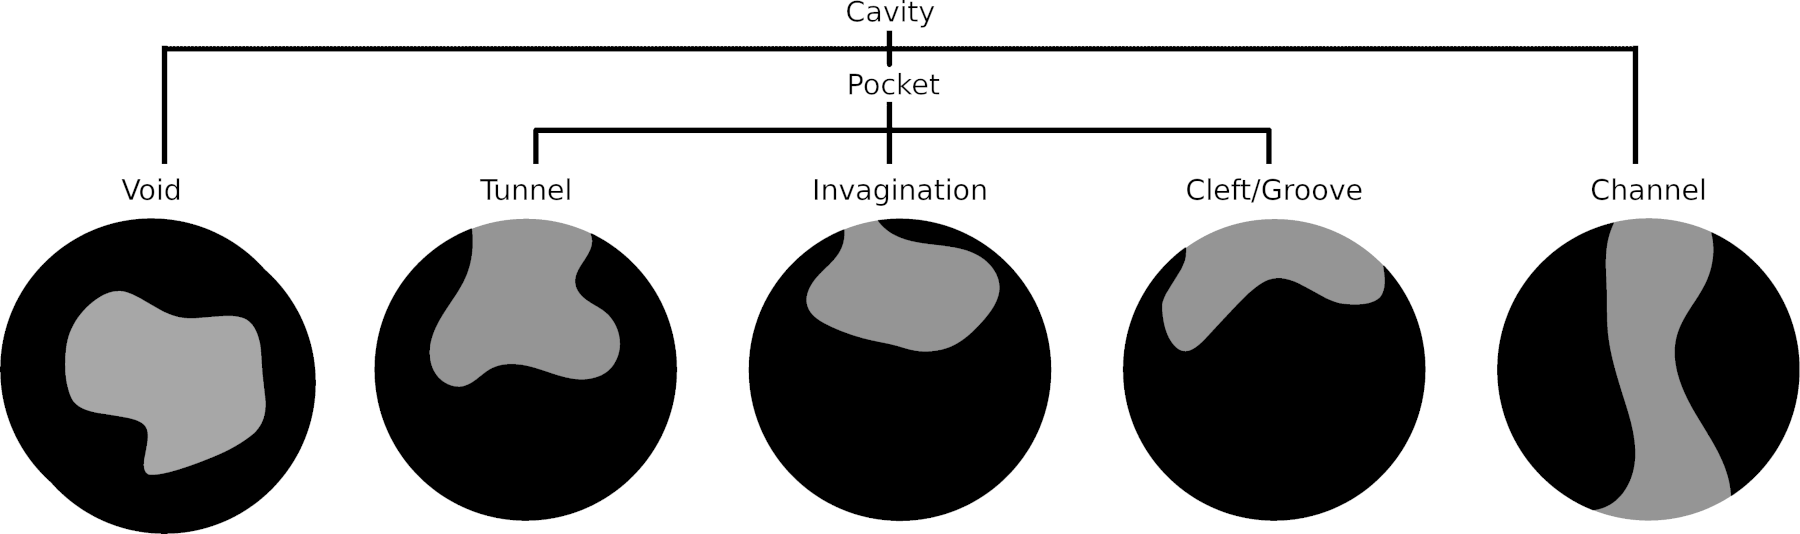
\includegraphics[scale=1]{images/cavity-classification.png}}
  \caption[Types of biomolecular cavities]{\textbf{Types of biomolecular cavities.} A biomolecular cavity (gray region) as a contiguous segment within the complement space of the biomolecule (black region), as defined by \cite{lay2013}. The categorization of these cavities follows an n-ary classification, where 'n' denotes the number of mouth openings. Specifically, a 0-ary cavity is identified as a void, representing an enclosed spatial configuration without external openings. In contrast, a 1-ary cavity, illustrated by a pocket, includes a single mouth opening. It is noteworthy that pockets encompass diverse forms like tunnels, invaginations, clefts, and grooves. Meanwhile, a 2-ary cavity, exemplified by a channel, features two mouth openings, facilitating the transit of molecular entities \cite{simoes2017}.}
  \label{fig:cavity-classification}
\end{figure}

In the current era of data science, the fields of computational and structural biology have significantly benefited from the increasing availability of biostructural data, as highlighted by \cite{mura2018}: "Structural biology meets data science". Advances in X-ray crystallography and electron microscopy techniques have expanded the determination of novel structures with respect to quality and size of these structures \cite{burley2018}. Biomolecules actively participate in various biological processes, such as protein folding, enzyme catalysis, DNA replication, DNA repair, cell signaling, virus-host interactions, and drug resistance. Dysregulation of these interactions is associated with numerous pathologies, including cancer, metabolic disorders, and pathogenic diseases \cite{scott2013}. For this reason, the identification and characterization of ligand-binding sites are the basis of rational structure-based drug discovery and design \cite{sotriffer2002,henrich2010}. Therefore, the imperative to identify targetable regions within the interaction area for new drugs becomes more apparent each day.

\section{Binding Site Characterization \label{sec:biomolecular-characterization}}

% The efficiency of identifying all cavities within a target protein using purely geometric approaches is noteworthy. However, the complexity arises in discriminating which of these cavities serve as functionally relevant binding sites \cite{sotriffer2002,henrich2010,liang1998,guerra2019}. While there is no simple and universally effective approach, characterizing binding sites based on their properties can lead to the identification of functionally relevant ones. As interactions within a cavity are inherently linked to its properties, elucidating these interactions becomes indispensable for determining the biological function of the biomolecule \cite{sotriffer2002,henrich2010}. 

Biomolecular interactions (\eg, \acs{PPI}, \acs{PLI}, \acs{PRI}, and \acs{PDI}) arise from distinctive property fingerprints at native or transient binding sites, where the molecular recognition hinges on the morphological, topological and physicochemical complementarity between the target biomolecule and its binding partner \cite{sotriffer2002,henrich2010,guerra2019,krone2016}. Binding sites impose morphological, topological and physicochemical constraints on putative ligands, with each interaction triggering a distinct biological function. Thus, describing potential binding sites in terms of morphological, topological, and physicochemical characteristics becomes essential for rational drug discovery and design, and assessing binding site druggability \cite{hubbard1994,liang1998,guerra2019,krone2016}.

The morphological attributes of biomolecular cavities establish stringent constraints on the geometry profiles of ligands capable of interacting efficiently within them. High affinity between the binding site and potential binders relies on sufficiently large interaction interfaces---extensive surface areas within the biomolecular cavity. The specificity of the binding site is dictated by geometric restrictions, including shape, size, and burial extent \cite{laskowski1996,liang1998}. Importantly, the cavity volume must accommodate the potential ligand \cite{stank2016}. The shape complementarity between the receptor and the ligand plays a decisive role in the binding process, with small ligands typically binding to buried concave sites on the molecular surface \cite{henrich2010}. Empirical studies have revealed that the active site often constitutes the largest and deepest cavity in enzymatic proteins \cite{laskowski1996}.

Topological characteristics of protein cavities contribute to functional analysis. The inference of the functionality of protein cavities has been achieved through comparison with homologous proteins, which exhibit homology and sequential similarity at the active site \cite{juncker2009}. Conserved local structural patterns, such as the catalytic triads of serine proteases \cite{dodson1998}, exemplify these homologous features. In enzymes, these specific configurations assume preferential spatial arrangements to execute elementary steps of the catalytic reaction, influencing the molecular recognition process of ligands by active sites \cite{sotriffer2002,henrich2010,thornton2000}. Describing a protein cavity according to the location of its different types of residues---hydrogen donors, electron receptors, hydrophobic contacts, and aromatics---becomes an insightful approach. Binding sites exhibit conserved amino acid sequences within protein families, offering valuable functional information \cite{henrich2010}. Amino acid composition distinguishes enzymatic from non-enzymatic binding sites, revealing varying compositions across different proteins \cite{guerra2019,carlson2008}.

Physicochemical characteristics play an essential role in selecting energetically favorable interactions. The synergy of van der Waals, hydrophobic, electrostatic, hydrogen bonding, and solvation interactions creates an energetically favorable environment for the binding process \cite{henrich2010}. For instance, hydrophobicity, quantified by the partition coefficient P, influences the kinetic and dynamic characteristics of drug action \cite{mannhold2009}. It is modulated by the shape of the binding site and the exposed area of residues \cite{henrich2010}. Various approaches generate distinct hydrophobicity scales for amino acids \cite{heiden1993}, such as Eisenberg \& Weiss \cite{eisenberg1984}, Hessa \& Heijne \cite{hessa2005}, Kyte \& Doolittle \cite{kyte1982}, Moon \& Fleming \cite{moon2011}, Radzicka \& Wolfenden \cite{radzicka1988}, Wimley \& White \cite{wimley1996}, and Zhao \& London \cite{zhao2006}. Conversely, the electrostatic potential, calculated by the Poisson-Boltzmann equation \cite{honig1995}, estimates ligand anchoring points, interaction free energy, biomolecule stability, and average atomic forces.

Therefore, the complexity lies in the discrimination which of these regions serve as functionally relevant binding sites, prompting the characterization of binding sites based on their distinctive properties \cite{sotriffer2002,henrich2010,liang1998,guerra2019}. Biomolecular interactions, shaped by morphological, topological, and physicochemical complementarity, form the foundation for understanding the biological function of biomolecules. While there is no simple and universally effective approach, characterizing binding sites based on their properties can lead to the identification of functionally relevant ones. As we unravel the intricate interplay of these properties, we gain essential insights into rational drug discovery, design, and the assessment of binding site druggability, marking a pivotal step toward advancing biomolecular research and therapeutic interventions \cite{sotriffer2002,henrich2010}.

\section{State of the Art \label{sec:state-of-the-art}}

Over the past decades, various \textit{in silico} have been developed for identifying binding sites in proteins to deepen our knowledge of a specific protein's function and for drug discovery and design \cite{liang1998}. However, only a few methodologies are applicable to other types of biomolecules, such as nucleic acids, carbohydrates, and lipids. The published computational approaches can be divided into three main categories: evolutionary, energetic, and geometric \cite{oliveira2014,simoes2017,guerra2019}.

\begin{itemize}
  \item \textbf{Evolutionary methods:} are based on the search for conserved residues in multiple sequence alignments and information from known binding site profiles;
  \item \textbf{Energetic methods:} identify binding sites based on the energetic interaction between the target biomolecule and a chemical probe, usually a chemical group;
  \item \textbf{Geometric methods:} identify cavities by analyzing the geometric characteristics of the molecular surface.
\end{itemize}

Each category of methods has its own advantages and disadvantages \cite{sotriffer2002,henrich2010,simoes2017}. Evolutionary algorithms heavily depend on sequence information or databases of active binding sites and the quality of the alignment procedure, while energetic methods rely on filtering procedures, force field parametrization, and applied scoring functions. On the other hand, geometric detection methods are relatively simple and straightforward, requiring no non-geometric knowledge, only structural data of the protein, \ie, the file in \ac{PDB}, XYZ, \ac{mmCIF}, or equivalent format, containing the Cartesian coordinates of atoms, easily accessible through the \ac{wwPDB}. Once atom coordinates are available, geometric methods should be able to represent any type of biomolecule \cite{henrich2010,oliveira2014,simoes2017}. Although purely geometric methods are efficient in identifying all types of cavities in a target molecule, identifying those that are functionally relevant poses a challenge. However, characterizing cavities in terms of well-chosen morphological, topological and physicochemical properties can lead to the identification of functionally relevant cavities, \ie, binding sites for a specific set of ligands \cite{sotriffer2002,henrich2010,liang1998,guerra2019}. 

In this context, geometry-based algorithms are the most widely used in the literature, as it is simple, direct, and does not require prior knowledge \cite{henrich2010,oliveira2014}. While evolution-based methods would be limited to proteins because they depend on principles of biological evolution, energy-based methods could be applicable but would require fine-tuning of force field parameters adapted to other types of biomolecules. As nucleic acids, carbohydrates, and lipids may have distinct properties compared to proteins, methods that rely solely on geometric information (e.g., \acs{3D} Cartesian coordinates and atom size) are desirable.

\subsection{Geometric Approaches \label{sec:geometric-approaches}}

The detection of cavities through geometric approaches is widespread, encompassing various techniques \cite{simoes2017,guerra2020}. These techniques are simple, straightforward, and do not require prior knowledge, making them the most commonly used in the literature \cite{henrich2010,oliveira2014}. In this context, we present a brief classification of geometric approaches for cavity detection (Figure \ref{fig:cavity-methods-infographic}), including techniques based on \ac{3D} grids, probes, surface, tessellation and their combinations \cite{simoes2017,guerra2020,guerra2023B}.

\begin{figure}[ht]
  \centering
  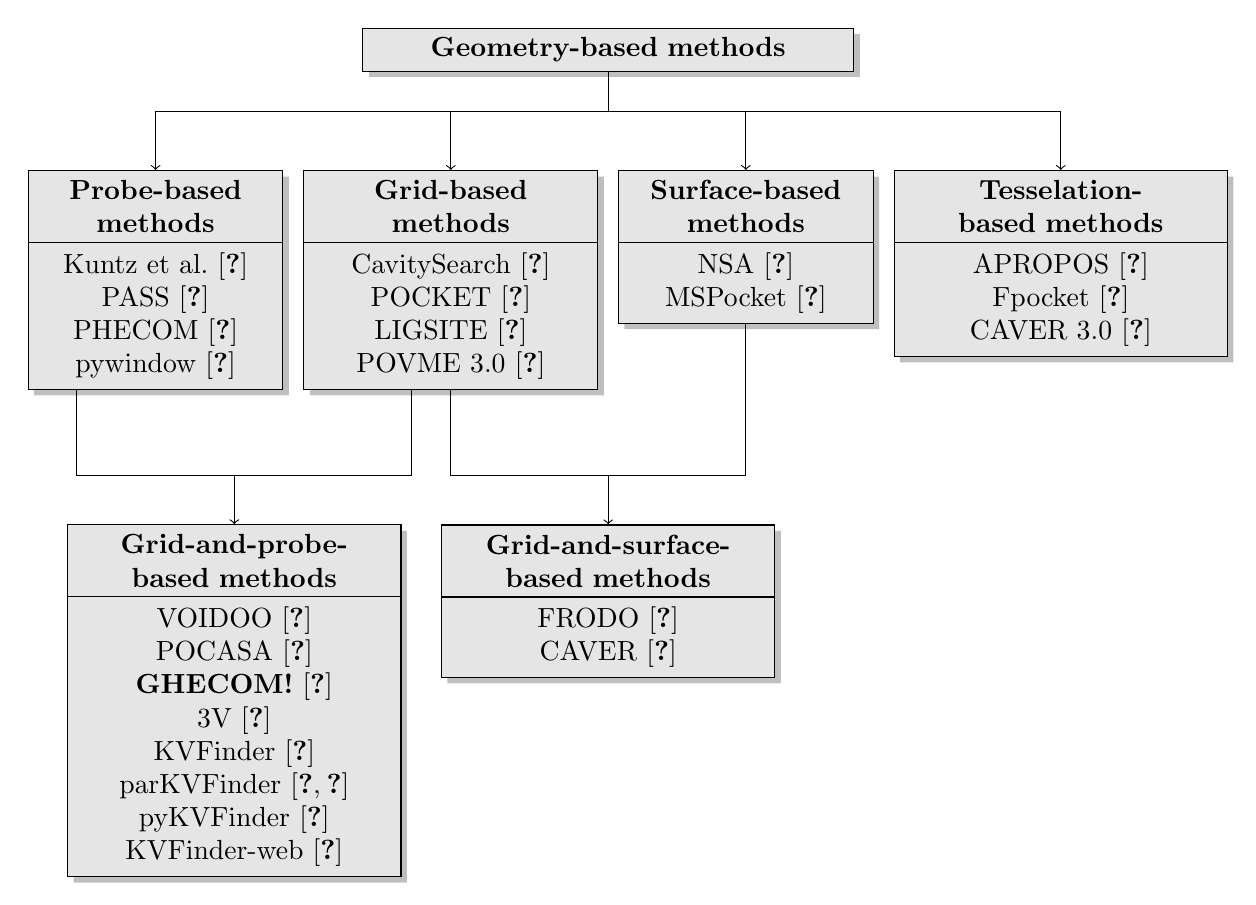
\begin{tikzpicture}[node distance=0.5cm]

    \node (GeomBased) [BoxNode, text width=6cm] {\textbf{Geometry-based methods}};
    \node (AuxNode01) [below=of GeomBased] {};
    \node (ProbeBased) [BoxNode, text width=3cm, rectangle split, rectangle split parts=2, below left=0.5cm and 4cm of AuxNode01] 
    {
      \textbf{Probe-based methods}
      \nodepart{two}{Kuntz et al. \ignorecitefornumbering{\cite{kuntz1982}}\\ PASS \ignorecitefornumbering{\cite{pass}}\\ PHECOM \ignorecitefornumbering{\cite{phecom}}\\ pywindow \ignorecitefornumbering{\cite{pywindow}}}
    };
    \node (GridBased) [BoxNode, text width=3.5cm, rectangle split, rectangle split parts=2, below left=0.5cm and 0cm of AuxNode01]
    {
      \textbf{Grid-based methods}
      \nodepart{two}{CavitySearch \ignorecitefornumbering{\cite{cavitysearch}}\\ POCKET \ignorecitefornumbering{\cite{pocket}}\\ LIGSITE \ignorecitefornumbering{\cite{ligsite}}\\ POVME 3.0 \ignorecitefornumbering{\cite{povme}}}
    };
    \node (SurfBased) [BoxNode, text width=3cm, rectangle split, rectangle split parts=2, below right=0.5cm and 0.0cm of AuxNode01]
    {
      \textbf{Surface-based methods}
      \nodepart{two}{NSA \ignorecitefornumbering{\cite{nsa}}\\ MSPocket \ignorecitefornumbering{\cite{mspocket}}}
    };
    \node (TessBased) [BoxNode, text width=4cm, rectangle split, rectangle split parts=2, below right=0.5cm and 3.5cm of AuxNode01]
    {
      \textbf{Tesselation-based methods}
      \nodepart{two}{APROPOS \ignorecitefornumbering{\cite{apropos}}\\ Fpocket \ignorecitefornumbering{\cite{fpocket}}\\ CAVER 3.0 \ignorecitefornumbering{\cite{caver3}}}
    };
    \node (AuxNode02) [below left=4.25cm and 4.7cm of AuxNode01] {};
    \node (AuxNode03) [below left=4.25cm and 4.3cm of AuxNode01] {};
    \node (AuxNode04) [below left=4.25cm and 4.5cm of AuxNode01] {};
    \node (GPBased) [BoxNode, rectangle split, rectangle split parts=2, below=0.5cm of AuxNode04, text width=4cm]
    {
      \textbf{Grid-and-probe-based methods}
      \nodepart{two}{VOIDOO \ignorecitefornumbering{\cite{voidoo}}\\ POCASA \ignorecitefornumbering{\cite{pocasa}}\\ \acs{GHECOM} \ignorecitefornumbering{\cite{ghecom}}\\ 3V \ignorecitefornumbering{\cite{3v}}\\ KVFinder \ignorecitefornumbering{\cite{oliveira2014}}\\ parKVFinder \ignorecitefornumbering{\cite{guerra2019,guerra2020}}\\ pyKVFinder \ignorecitefornumbering{\cite{guerra2021}}\\ KVFinder-web \ignorecitefornumbering{\cite{guerra2023A}}}
    };
    \node (GSBased) [BoxNode, rectangle split, rectangle split parts=2, below=5cm of AuxNode01, text width=4cm]
    {
      \textbf{Grid-and-surface-based methods}
      \nodepart{two}{FRODO \ignorecitefornumbering{\cite{frodo}}\\ CAVER \ignorecitefornumbering{\cite{caver}}}
    };
    \node (AuxNode05) [below left=4.25cm and 0.0cm of AuxNode01] {};
    \node (AuxNode06) [below right=4.25cm and 0.0cm of AuxNode01] {};
    \node (AuxNode07) [below=4.25cm of AuxNode01] {};

    \draw [->] (GeomBased.south) -- (AuxNode01)+(0,0.12) -| (ProbeBased.north);
    \draw [->] (GeomBased.south) -- (AuxNode01)+(0,0.12) -| (GridBased.north);
    \draw [->] (GeomBased.south) -- (AuxNode01)+(0,0.12) -| (SurfBased.north);
    \draw [->] (GeomBased.south) -- (AuxNode01)+(0,0.12) -| (TessBased.north);
    \draw [-] (ProbeBased.south)+(-1,0) |- (AuxNode03);
    \draw [->] (GridBased.south)+(-0.5,0) |- (AuxNode02)-| (GPBased.north);
    \draw [-] (SurfBased.south)+(0,0) |- (AuxNode05);
    \draw [->] (GridBased.south)+(0,0) |- (AuxNode06)-| (GSBased.north);

  \end{tikzpicture}
  \caption[Classification of geometry-based methods]{\textbf{Classification of geometry-based methods.}}
  \label{fig:cavity-methods-infographic}
\end{figure}

\begin{itemize}
  \item \textbf{Grid-based algorithms} (\eg, CavitySearch \cite{cavitysearch}, POCKET \cite{pocket}, LIGSITE \cite{ligsite}, POVME 3.0 \cite{povme}) represent a set of atoms as discrete points, usually using a \acs{3D} grid aligned to the axes as a scalar field, \ie, a density map, where each discrete point is an integer or boolean value. These grid maps are used to cluster relevant empty space points (\ie, not belonging to the solute) into cavities using voxel clustering algorithms. Typically, these methods use simple data structures capable of representing a collection of data at a discrete point and identifying cavities automatically. However, geometric accuracy, computation time, and memory consumption heavily depend on the grid resolution, \ie, grid-spacing sensitivity. Additionally, these methods are not rotationally invariant, meaning that the orientation of a given molecule slightly affects accuracy, \ie, orientation sensitivity;
  \item \textbf{Probe-based algorithms} (\eg, Kuntz et al. \cite{kuntz1982}, PASS \cite{pass}, PHECOM \cite{phecom}, pywindow \cite{pywindow}) use a set of atoms, considering their \acs{3D} coordinates and \ac{vdW} radii, to represent the molecular surface, which is analyzed by one or more probes, usually rigid spheres, to investigate its accessibility levels. This technique can detect any type of cavity and is related to the spatial extension of potential ligands; however, it may struggle to find and unequivocally delineate the boundaries between the cavity and the solvent, \ie, mouth-opening ambiguity;
  \item \textbf{Surface-based algorithms} (\eg, NSA \cite{nsa}, MSPocket \cite{mspocket}) do not use a rigid sphere model but rather a molecular surface model, such as \acs{vdW} surface, \ac{SES}, \ac{SAS}, and \ac{LES}, defining the molecular interface and its environment. Analysis of the molecular interface identifies cavities based on accessibility to a specific solvent or ligand. In this case, cavity detection occurs automatically, as in grid-based methods, but without mouth-opening ambiguity. However, in some cases, these algorithms may struggle to detect all types of cavities and their complete extent;
  \item \textbf{Tessellation-based algorithms} (\eg, APROPOS \cite{apropos}, Fpocket \cite{fpocket}, CAVER 3.0 \cite{caver3}) rely on computational geometry techniques, such as \textalpha-shapes, \textbeta-shapes, Voronoi diagrams, and Apollonius diagrams. Specifically, \textalpha-shapes and Voronoi tessellation use atomic centers, implicitly constant-radius spheres to model atoms, while \textbeta-shapes and Apollonius-based methods depend on variable-radius spheres to model these atoms, which are explored to identify cavities. Typically, these methods do not depend on any information from the molecular surface to detect cavities but may struggle to identify the correct binding site location, delineate the boundaries between the cavity and the solvent, and define the number of surface atoms.
\end{itemize}

This classification illustrates that each technique has its own inherent strengths and weaknesses, rendering them more suitable for specific applications \cite{simoes2017,guerra2020}. The cohesive combination of these techniques aims to leverage the capabilities of each and mitigate their individual shortcomings, resulting in more robust approaches. Within this broader context, two notable subcategories emerge:

\begin{itemize}
  \item \textbf{Grid-and-probe-based methods} (\eg, VOIDOO \cite{voidoo}, POCASA \cite{pocasa}, \acs{GHECOM} \cite{ghecom}, 3V \cite{3v}, KVFinder \cite{oliveira2014}, parKVFinder \cite{guerra2019,guerra2020}) combine the strengths of both grid- and probe-based methods. Analogous to grid-based methods, they rely on a scalar field defined at each grid point and predominantly use large probe spheres rolling on the \acs{vdW} surface. These probes define cavities between the probe-generated surface and the molecular surface. This combined approach mitigates mouth-opening ambiguity and orientation sensitivity, common in grid-based methods \cite{simoes2017}. The mouth-opening ambiguity is also known as cavity ceiling problem, which can be controlled by customizable probe sizes \cite{simoes2017,oliveira2014}. However, grid-spacing sensitivity remains, unless we use a grid spacing of at most half of the smaller probe to mitigate it. The usage of probes in grid-based methods follows three techniques, that are atom fattening (originating \acs{SAS} or \acs{SAS}-like surfaces), exemplified by VOIDOO \cite{voidoo}, rolling probes of unequal radii on the \acs{vdW} surface, as seen in POCASA \cite{pocasa}, \acs{GHECOM} \cite{ghecom}, and 3V \cite{3v}, and concentric probes of unequal radii at grid points, specifically implemented in KVFinder software \cite{oliveira2014};
  \item \textbf{Grid-and-surface-based methods} (\eg, FRODO \cite{frodo}, CAVER \cite{caver}) combine the strengths of both grid- and surface-based methods. Similar to probe spheres, surfaces resolve the ambiguity issue in grid-based methods, particularly in defining cavity ceilings (and, consequently, mouth openings). These methods employ a scalar field in conjunction with a \acs{3D} grid, where the scalar field may be defined by various functions. In summary, the utilization of surfaces with grids overcomes common issues associated with grid-based methods, namely, orientation sensitivity and mouth-opening ambiguity. However, the challenge of grid-spacing sensitivity persists unless a grid spacing of at most half of the smaller probe.
\end{itemize}

In this context, the exploration of geometric approaches for cavity detection reveals a diverse landscape of techniques, each with its unique strengths and weaknesses. The simplicity and accessibility of these methods have made them foundational in biomolecular research \cite{henrich2010,simoes2017}. This classification, encompassing grid-based, probe-based, surface-based, and tessellation-based algorithms, provides a comprehensive overview of the strategies employed in structural and functional characterization of biomolecules and binding sites \cite{simoes2017}. The cohesive integration of these techniques, as seen in grid-and-probe-based or grid-and-surface-based methods, represents a strategic effort to overcome individual limitations and enhance the robustness of cavity detection methodologies. By acknowledging the strengths of each approach and strategically combining them, researchers aim to optimize the efficacy of computational platforms, paving the way for more nuanced and accurate structural and functional insights into biomolecules.

\subsection{Well-established Computational Tools \label{sec:computational-tools}}

The vast majority of cavity detection tools were originally developed for proteins (see Section \ref{sec:geometric-approaches}). Although these algorithms exhibit robustness in describing and analyzing any molecular system (\eg, protein, DNA, RNA, inorganic material, supramolecular cage, etc.), so far, only a few tools have been applied to other biomolecular systems, excluding proteins, to assess structural characteristics such as the shape, volume, area and mouth openings. Our literature review led us to identify tools meeting specific criteria: applicability to any molecular system, availability as free software, comprehensive documentation, robust developer support, a well-conceived set of characterizations, and recognition within the scientific community. Guided by these stringent criteria, we spotlight four well-established cavity detection tools: parKVFinder, Fpocket, \acs{GHECOM}, and CAVER tools.

\subsubsection{parKVFinder}

parKVFinder \cite{guerra2019,guerra2020}, a grid-and-probe-based approach, detects and characterizes any type of biomolecular cavity, integrated with a graphical plugin for PyMOL \cite{pymol}. The cavity detection algorithm (Figure \ref{fig:parkvfinder-schema}) employs a dual-probe methodology based on mathematical morphology theory \cite{matheron1974,serra1982}. Originally implemented in the KVFinder software \cite{oliveira2014}, this algorithm involves two probes, a smaller probe (\textit{Probe In}) and a larger probe (\textit{Probe Out}), inspecting grid points to define cavities as the non-overlapping regions traversed by these probes.

\begin{figure}[h]
  \centerline{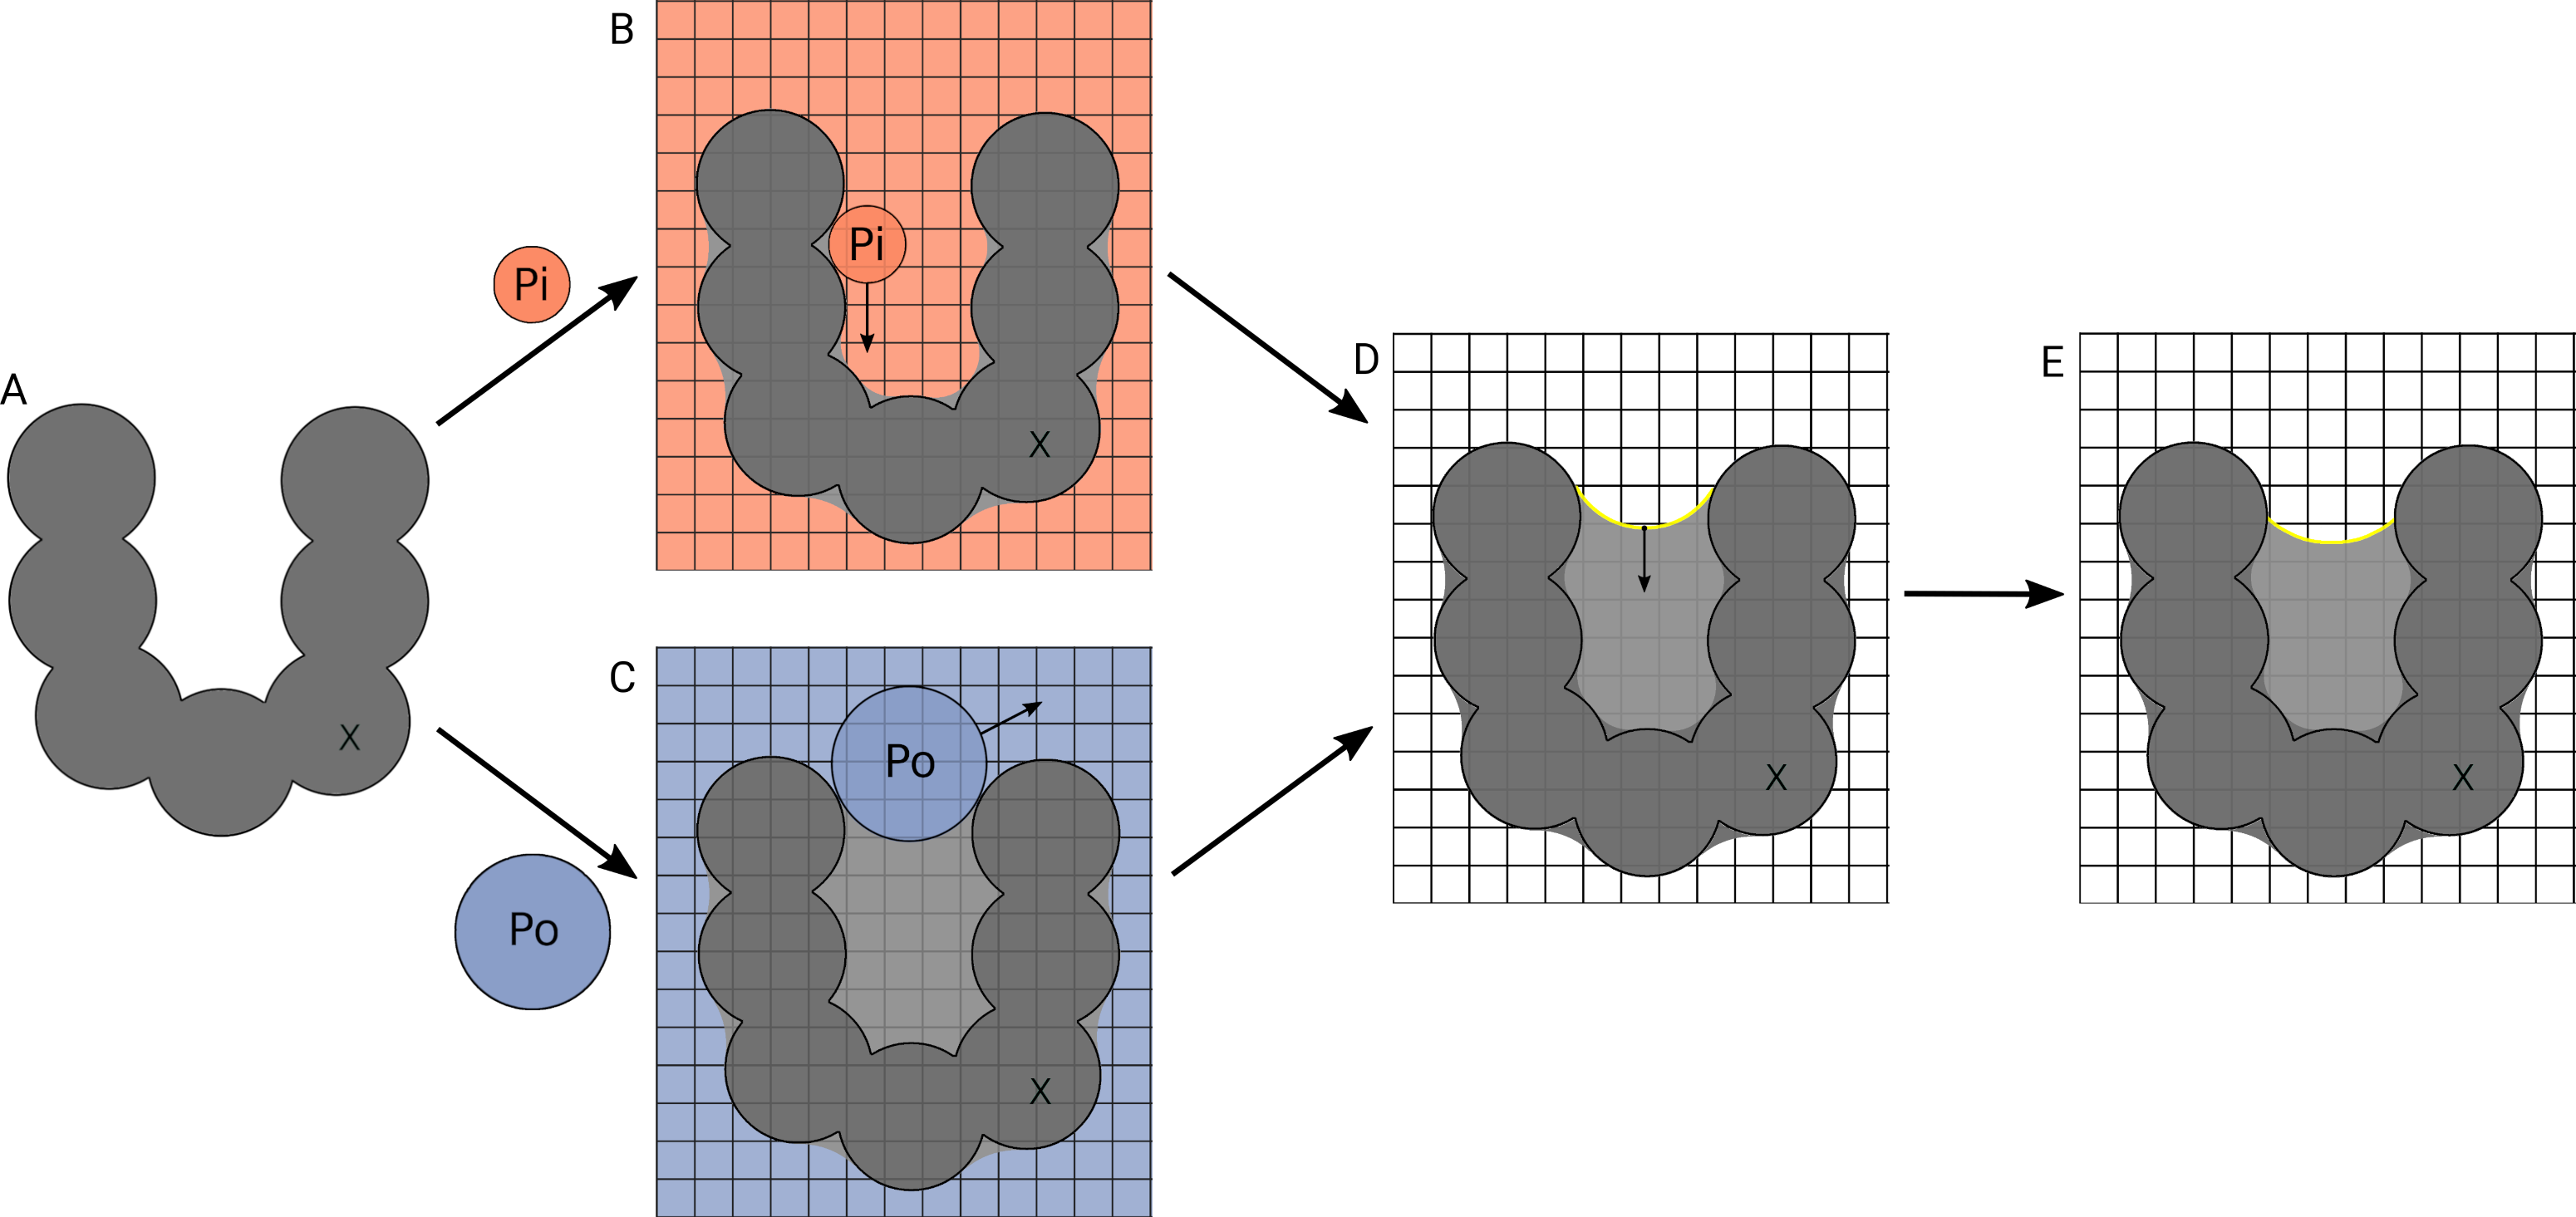
\includegraphics[scale=1]{images/kvfinder-suite-schema.png}}
  \centerline{\tiny{\textbf{Source:} Reprinted with permission from \cite{guerra2023B}. Copyright 2023 American Chemical Society.}}
  \caption[Cavity detection algorithm in parKVFinder]{\textbf{Cavity detection algorithm in parKVFinder.} \textbf{(A)} A biomolecular structure X, composed of atoms modeled as rigid spheres with van der Waals radii, is inserted into a \acs{3D} grid. \textbf{(B)} The \ac{Pi} probe traverses the surface of the structure, moving through grid points (orange). \textbf{(C)} Next, the \ac{Po} probe traverses accessible points in blue. \textbf{(D)} Cavity points (light gray) are defined as the difference between the accessible points of the probes. Points not reached by \acs{Pi} (dark gray) define the \acs{SES} (standard) or \acs{SAS}, depending on the surface representation chosen by the user. \textbf{(E)} Finally, a distance-based removal procedure is applied to eliminate cavity points near the cavity-bulk boundary (yellow line).}
  \label{fig:parkvfinder-schema}
\end{figure}

It is noteworthy that the original KVFinder software \cite{oliveira2014}, introduced in 2014, has been deprecated. However, subsequent implementations, namely parKVFinder \cite{guerra2020}, pyKVFinder \cite{guerra2021}, and KVFinder-web \cite{guerra2023A}, have been developed to enhance computational performance and usability. Each of these tools addresses different scientific community demands in a flexible manner. Cavity characterization in these tools includes morphological descriptors (\eg, volume, area, shape, and depth), topological descriptors (\eg, interface residues surrounding the cavities and their classification---aliphatic, aromatic, polar uncharged, negatively charged, and positively charged---), and physicochemical descriptors (\eg, hydrophobicity). Further details on the parKVFinder can be found in Section \ref{sec:parkvfinder}.

\subsubsection{Fpocket}

Fpocket \cite{fpocket}, a tessellation-based approach, employs the concept of \textalpha\space spheres, originally introduced by \cite{liang1998}, for the detection of molecular pockets. The cavity detection algorithm (Figure \ref{fig:fpocket-schema}) performs a comprehensive analysis to identify the whole set of \textalpha\space spheres within a given molecular structure, using the \textit{qhull} package \cite{qhull}. The process involves categorizing small alpha spheres situated inside the structure, large spheres outside the structure, and the spheres in between as corresponding to cavities. To refine the cavity selection, Fpocket eliminates any alpha sphere falling outside a customized range of minimum and maximum radii. The remaining \textalpha\space spheres are grouped into cavities based on proximity and neighborhood relationships, and cavities of poor interest (\eg, hydrophilic or small putative pockets) excluded from further analysis. Subsequently, the cavities are assessed using a set of dpocket descriptors \cite{fpocket}, allowing the cavities to be ranked according to their putative binding affinity for small molecules. 

\begin{figure}[ht]
  \centerline{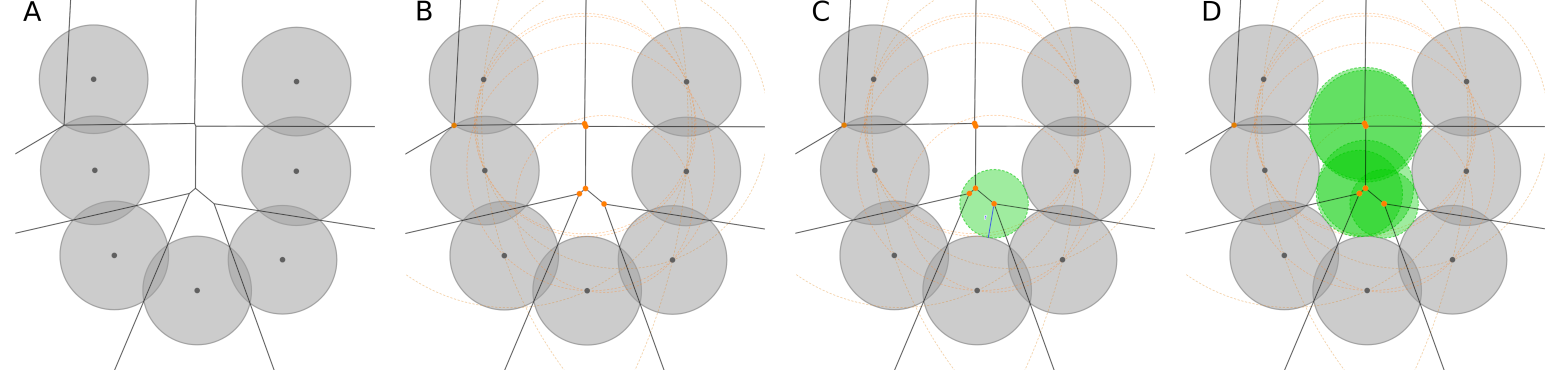
\includegraphics[scale=0.9]{images/fpocket-schema.png}}
  \centerline{\tiny{\textbf{Source:} Reprinted with permission from \cite{guerra2023B}. Copyright 2023 American Chemical Society.}}
  \caption[Cavity detection algorithm in Fpocket]{\textbf{Cavity detection algorithm in Fpocket.} \textbf{(A)} Voronoi diagram of the atomic centers. \textbf{(B)} Voronoi balls (dotted orange circles) centered at Voronoi vertices (orange points). \textbf{(C)} Example of an \textalpha\space sphere (green sphere) centered at a Voronoi vertex (orange point) and grows until it becomes tangent to an atom. \textbf{(D)} Cluster of \textalpha\space spheres (green region) filling the binding site.}
  \label{fig:fpocket-schema}
\end{figure}

\subsubsection{\acs{GHECOM}}

\ac{GHECOM} \cite{ghecom}, a grid-and-probe-based approach, identifies both deep and shallow pockets, employing an array of spherical probes. The cavity detection algorithm (Figure \ref{fig:ghecom-schema}) combines fundamental erosion and dilation operations from mathematical morphology \cite{matheron1974,serra1982} with different spherical probes to report openness-closedness of a target molecular shape, thereby revealing deep and shallow pockets (referred to as \textit{multi-scale pockets}). Following that, a single-linkage clustering method groups pocket regions, allowing for the subsequent estimation of their respective volumes. \acs{GHECOM} introduces a metric known as \textit{pocketness}, which establishes a correlation between the volume and depth of points associated with individual residues or atoms. This metric serves as an informative indicator of their respective contributions to ligand interactions.

\begin{figure}[H]
  \centerline{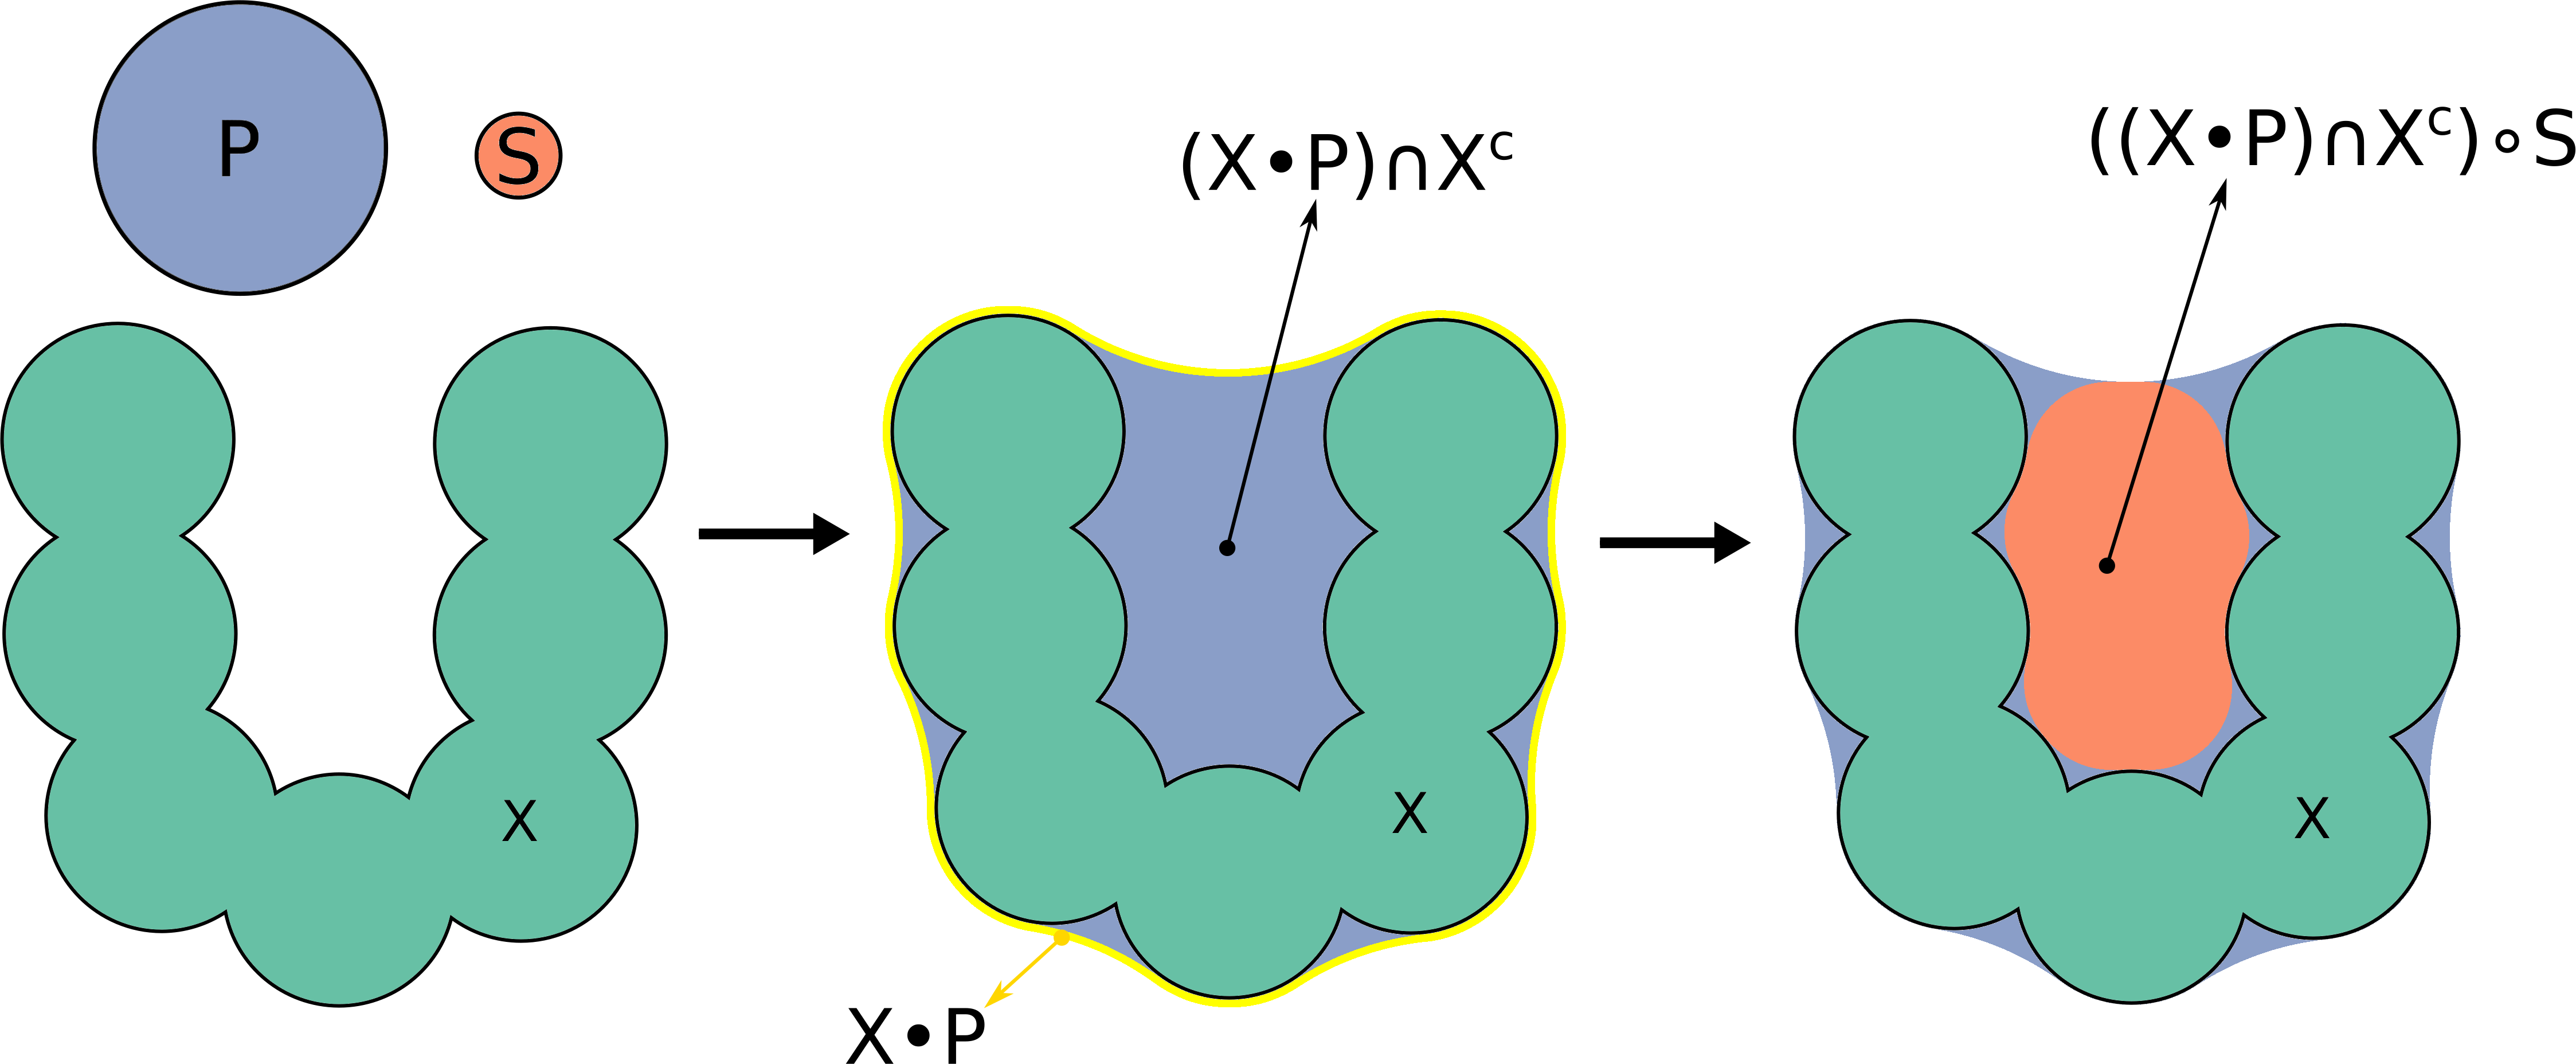
\includegraphics[scale=0.9]{images/ghecom-schema.png}}
  \centerline{\tiny{\textbf{Source:} Reprinted with permission from \cite{guerra2023B}. Copyright 2023 American Chemical Society.}}
  \caption[Pocket detection algorithm in \acs{GHECOM}]{\textbf{Pocket detection algorithm in \acs{GHECOM}.} A biomolecular structure (green region; $X$) is enclosed by a spherical probe P (blue sphere), defining the region bounded by the yellow contour. Next, the intersection of X closed by P ($X \bullet P$) and the space outside the protein ($X^c$) defines the region not accessible to the probe P (blue region; $(X \bullet P) \cap X^c$). Subsequently, this region is opened by a spherical probe S (orange sphere), where P is larger than S. Finally, the pocket (orange region; $((X \bullet P) \cap X^c) \circ S$) is defined by the space outside the molecular shape not accessible to P but accessible to S. For multi-scale detection, different sizes of the spherical probe P are used.}
  \label{fig:ghecom-schema}
\end{figure}

\subsubsection{CAVER tools}

CAVER tools comprise a series of computational methods designed for tunnel and channel analysis within biomolecular structures. The initial iteration, CAVER \cite{caver}, was a grid-and-surface-based approach for tunnel and channel calculation. Subsequently, CAVER 3.0 \cite{caver3} replaced the axis-aligned grid with a Voronoi diagram approach, turning into a tessellation-based approach. The user-friendly interface, CAVER Analyst 2.0 \cite{caveranalyst2}, incorporates CAVER 3.0, providing visual assistance to users in tunnel and cavity calculations. The cavity detection algorithm (Figure \ref{fig:caver-schema}) constructs a pseudo-Voronoi diagram of a given biomolecular structure. By identifying paths represented as graphs composed of Voronoi vertices and edges, CAVER 3.0 characterizes these paths as tunnels connecting cavities to the surrounding solvent. The resulting tunnels are further characterized by length, average radius, and bottleneck (mouth opening) radius. CAVER Analyst 2.0 complements these functionalities by identifying regions of empty space (\ie, cavities) within the biomolecular structure. Employing a similar approach to that described in the KVFinder suite (Figure \ref{fig:parkvfinder-schema}) and \acs{GHECOM} (Figure \ref{fig:ghecom-schema}), CAVER Analyst 2.0 determines regions accessible where a small probe can enter from outside, but a large probe cannot.

\begin{figure}[H]
  \centerline{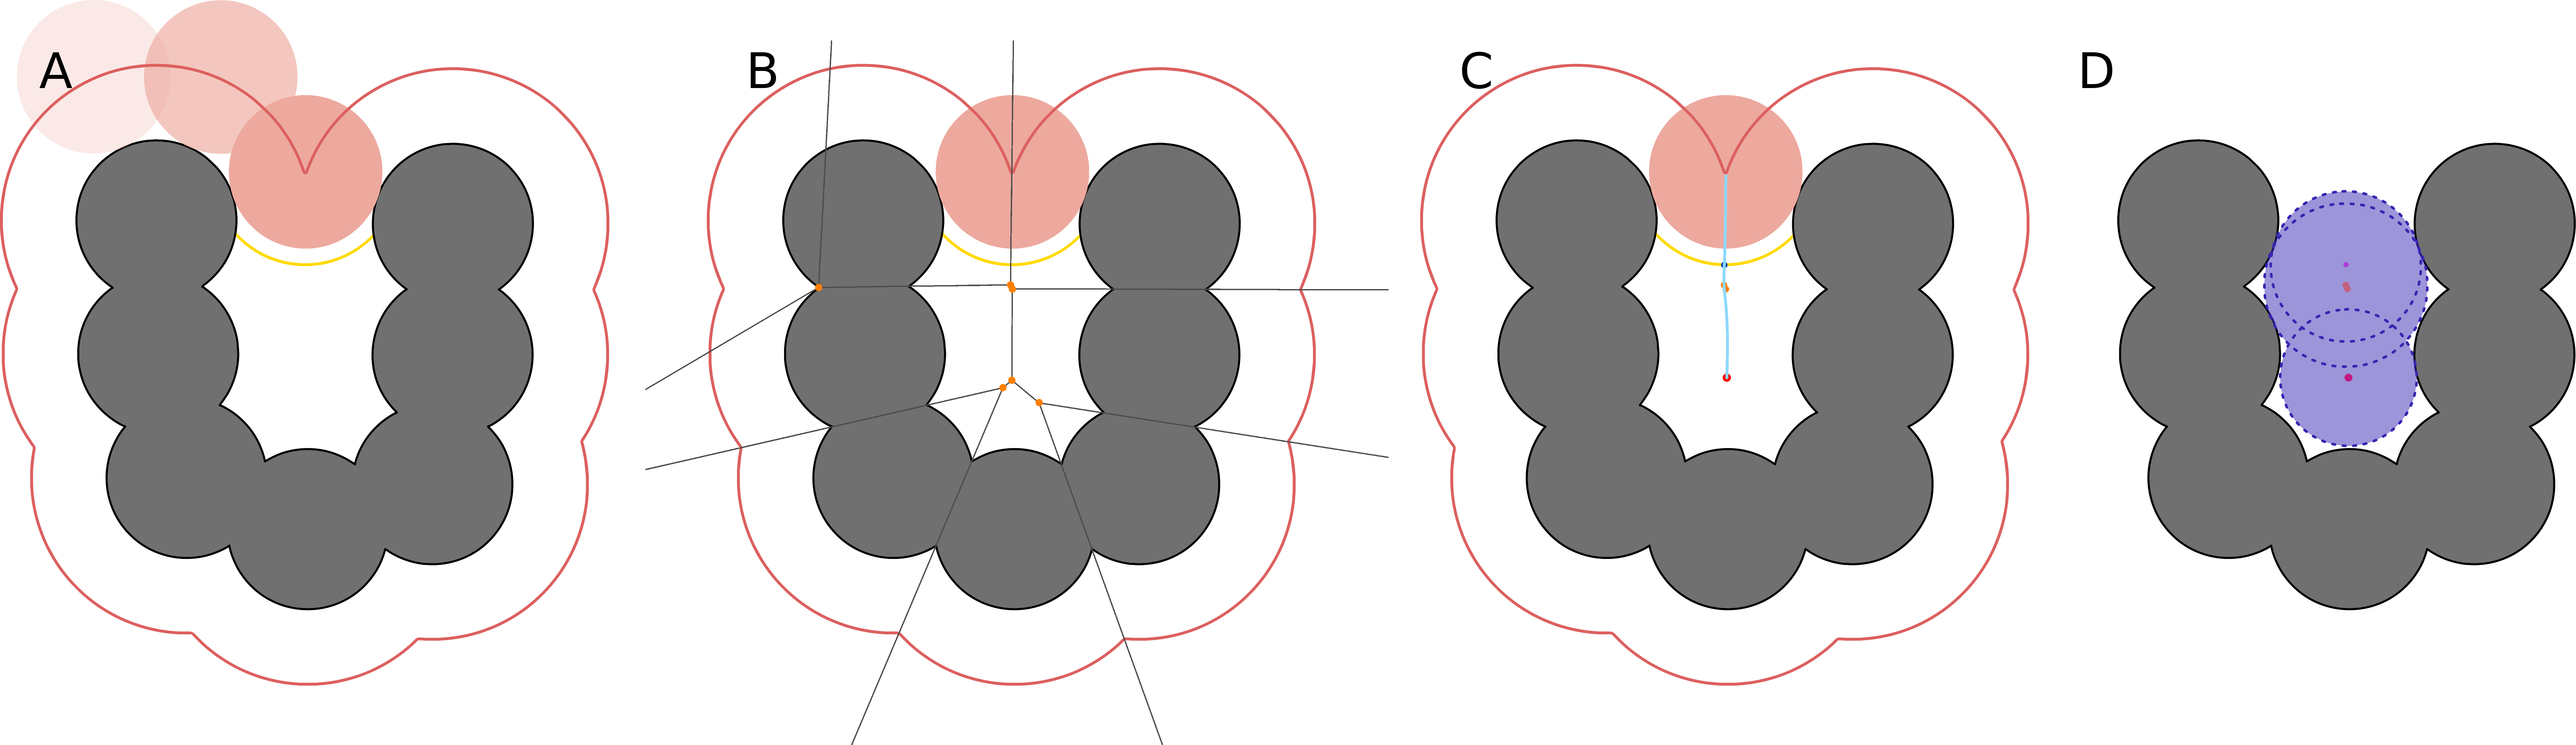
\includegraphics[scale=1.1]{images/caver-schema.png}}
  \centerline{\tiny{\textbf{Source:} Reprinted with permission from \cite{guerra2023B}. Copyright 2023 American Chemical Society.}}
  \caption[Channel and tunnel detection algorithm in CAVER 3.0]{\textbf{Channel and tunnel detection algorithm in CAVER 3.0.} \textbf{(A)} A molecular shape is probed by a spherical probe, called the \textit{shell probe}, with a radius specified by the \textit{shell radius} parameter, to define an outer surface \acs{SAS} (red line). From it, a distance specified by the \textit{shell depth} parameter is removed to define an inner surface (yellow line). \textbf{(B)} A pseudo-Voronoi diagram is constructed based on the molecular shape. Voronoi vertices (orange points) are used to create the central lines of the tunnel/channel. \textbf{(C)} A starting point (red point) is a user-defined parameter set as the center of mass of the molecular shape, and an endpoint (blue point) is set at the center of the inner surface. From the starting point, the central line passes through Voronoi edges and vertices to form a tunnel/channel to the outer surface and passes through the endpoint. \textbf{(D)} Spheres are fitted at all points of the central line, from the starting point to the endpoint, defining the bottleneck (mouth opening) radius along the tunnel and/or channel.}
  \label{fig:caver-schema}
\end{figure}

\section{Computational Complexity \label{sec:computational-complexity}}

The effectiveness of cavity detection algorithms relies not only on their accuracy in identifying binding sites but also on their computational efficiency, particularly when dealing with biomolecular structures and large datasets. Computational complexity, a field studying algorithmic efficiency, involves analyzing the computational resources, such as time and space, required by an algorithm to solve a specific problem as a function of the input size. The goal is to understand how an algorithm's performance scales with increasing input sizes.

There are two primary aspects of computational complexity:

\begin{itemize}
  \item \textbf{Time Complexity:} measures the time an algorithm takes to complete relative to the input size;
  \item \textbf{Space Complexity:} measures the memory (\ie, space) an algorithm needs to solve a problem based on the input size.
\end{itemize}

In computer science, both time and space complexity are often expressed using big-O notation ($\mathcal{O}$), also known as Bachmann-Landau notation. This notation describes the upper bound of an algorithm's running time and memory requirements, respectively, classifying algorithms based on how their performance grows relative to the input size.

In this scenario, the computational complexity of cavity detection algorithms is a
critical aspect that influences their practical utility and scalability. Here, we briefly delve into the computational complexity of the geometry-based approaches described in Section \ref{sec:geometric-approaches}.

Grid-based algorithms (\eg, CavitySearch \cite{cavitysearch}, POVME 3.0 \cite{povme}) rely on discretizing the molecular structure into a \acs{3D} grid. The computational complexity of these methods is inherently tied to the grid spacing and biomolecule size. The time complexity is typically $\mathcal{O}(n_{v})$, where $n_{v}$ represents the number of voxels, and it linearly increases with the number of voxels. In terms of user inputs, the number of voxels (Eq. \ref{eq:nv-ref}) is expressed as follows:

\begin{equation}
  n_v \colon (l_x,l_y,l_z,s) \simeq \left \lceil \frac{l_x}{s} \right \rceil \cdot \left \lceil \frac{l_y}{s} \cdot \right \rceil \left \lceil \frac{l_z}{s} \right \rceil
  \label{eq:nv-ref}
\end{equation}

\noindent where $l_x$, $l_y$, $l_z$ are the lengths of the target biomolecule along x, y, and z-axis, respectively, $s$ is the grid spacing, and $\lceil \cdot \rceil$ is the ceiling function.

A finer grid provides a more detailed representation of the molecular surface but increases the number of grid points to be processed. Consequently, there exists a delicate balance between achieving sufficient resolution for accurate cavity detection and maintaining computational efficiency. The spatial complexity, referring to the memory requirements, is also $\mathcal{O}(n_{v})$ as it scales with the number of voxels. Implementing strategies to optimize grid-based algorithms involves finding ways to reduce this linear relationship, such as through sparse grid representations or parallel processing.

Probe-based algorithms (\eg, PHECOM \cite{phecom}, pywindow \cite{pywindow}) introduce a distinct set of considerations, where the chosen probe size significantly influences precision and sensitivity in cavity detection. The time complexity of probe-based algorithms is often expressed as $\mathcal{O}(n_{p} \cdot n_{a})$, where $n_{p}$ is the number of probes, and $n_{a}$ is the number of atoms. Conversely, spatial complexity depends solely on the number of atoms, denoted as $\mathcal{O}(n_{a})$.

Surface-based algorithms (\eg, NSA \cite{nsa}, MSPocket \cite{mspocket}) focus on the molecular surface characteristics. The computational complexity of surface-based algorithms is associated with the surface representation and analysis techniques employed. These methods typically involve operations on the molecular surface mesh or point cloud, leading to complexities that depend on factors such as surface resolution, mesh complexity, and the nature of surface analysis. These complexities can range from linear (\eg, vertex transformation) to polynomial (\eg, convex hull computation), and optimizations often revolve around efficient mesh processing and surface characterization techniques.

Tessellation-based algorithms (\eg, Fpocket \cite{fpocket} and CAVER 3.0 \cite{caver3}) leverage geometric techniques such as Voronoi diagrams and \textalpha\space spheres. The computational complexity here is intricately linked to the efficiency of these geometric operations. The time complexity of tessellation-based algorithms often involves complex geometric operations and is expressed as $\mathcal{O}(n_{a} \cdot \log{n_{a}})$, where $n_{a}$ is the number of atoms. Spatial complexity depends on the number of points (\ie, number of atoms) used in the geometric calculations, expressed as $\mathcal{O}(n_{a})$.

Thus, systematic evaluation of the computational complexity inherent in a given algorithm presents their limitations but also unveils opportunities for optimization. The intrinsic complexity of biomolecular systems requires the development of efficient algorithms capable of handling large datasets. In this context, parallel computing emerges as a promising avenue for enhancing the computational efficiency of computational biology algorithms, including tasks such as cavity detection, cavity characterization, solvent accessibility determination, and beyond.

\section{Parallel Computing \label{sec:parallel-computing}}

Computational problems are typically divided into distinct parts, each comprising sets of instructions. In computing, two fundamental approaches exist: serial computing, which executes instructions sequentially, and parallel computing, which leverages multiple computational resources simultaneously (Figure \ref{fig:computing-strategies}). Parallel execution enables the simultaneous execution of instructions, thereby reducing computational time---a critical advantage in the context of modern computers featuring parallel architectures with multiple processors \cite{foster1995,grama2003}. Despite its potential, parallel computing introduces new challenges that necessitate careful consideration. Coordinating parallel tasks, managing data synchronization, and minimizing communication overhead are critical concerns. Load balancing becomes pivotal to ensure uniform resource utilization, preventing bottlenecks that hinder performance gains. Additionally, designing algorithms that effectively parallelize tasks is a complex endeavor, requiring a deep understanding of both the problem domain and the intricacies of parallel architectures \cite{grama2003,matloff2012}.

\begin{figure}[h]
  \raggedright
  \textbf{Serial Computing} \\
  \vspace{0.2cm}
  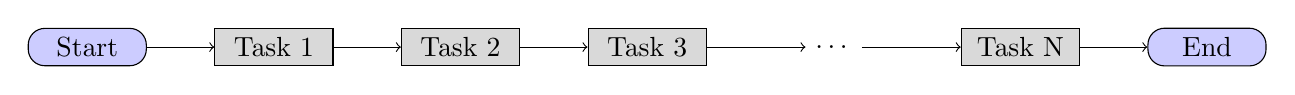
\begin{tikzpicture}[node distance=2.37cm]
      
    \node (start) [StartEndNode] {Start};
    \node (task1) [OperationNode, right of=start] {Task 1};
    \node (task2) [OperationNode, right of=task1] {Task 2};
    \node (task3) [OperationNode, right of=task2] {Task 3};
    \node (dots) [right of=task3] {\dots};
    \node (taskn) [OperationNode, right of=dots] {Task N};
    \node (end) [StartEndNode, right of=taskn] {End};
    
    \draw [->] (start) -- (task1);
    \draw [->] (task1) -- (task2);
    \draw [->] (task2) -- (task3);
    \draw [->] (task3) -- (dots);
    \draw [->] (dots) -- (taskn);
    \draw [->] (taskn) -- (end);
  \end{tikzpicture} \\ 
  \vspace{0.5cm} % Space between diagrams
  \textbf{Parallel Computing} \\
  \vspace{0.2cm}
  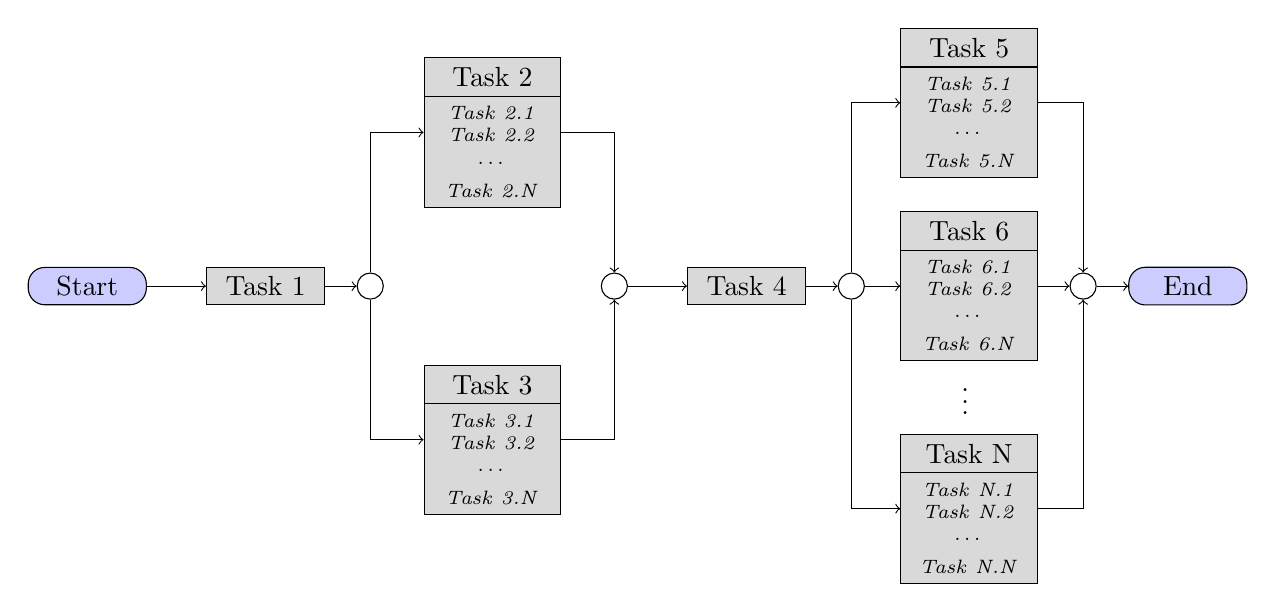
\begin{tikzpicture}[node distance=0.4cm]
    
    \node (start) [StartEndNode] {Start};
    \node (task1) [OperationNode, right=0.75cm of start] {Task 1};
    \node (ConnNode01) [ConnNode, right=of task1] {};
    \node (task2) [OperationNode, rectangle split, rectangle split parts=2, above right=0.75cm and 1.25cm of task1, text width=1.5cm, text centered] {
      Task 2
      \nodepart{two}{\scriptsize{\textit{Task 2.1}\\ \textit{Task 2.2}\\ \dots \\ \textit{Task 2.N}}}
    };
    \node (task3) [OperationNode, rectangle split, rectangle split parts=2, below right=0.75cm and 1.25cm of task1, text width=1.5cm, text centered] {
      Task 3
      \nodepart{two}{\scriptsize{\textit{Task 3.1}\\ \textit{Task 3.2}\\ \dots \\ \textit{Task 3.N}}}
    };
    \node (ConnNode02) [ConnNode, right=3.5cm of task1] {};
    \node (task4) [OperationNode, right=0.75cm of ConnNode02] {Task 4};
    \node (ConnNode03) [ConnNode, right=of task4] {};
    \node (task5) [OperationNode, rectangle split, rectangle split parts=2, above right=1.25cm and 0.5cm of ConnNode03, text width=1.5cm, text centered] {
      Task 5
      \nodepart{two}{\scriptsize{\textit{Task 5.1}\\ \textit{Task 5.2}\\ \dots \\ \textit{Task 5.N}}}
    };
    \node (task6) [OperationNode, rectangle split, rectangle split parts=2, right=0.45cm of ConnNode03, text width=1.5cm, text centered] {
      Task 6
      \nodepart{two}{\scriptsize{\textit{Task 6.1}\\ \textit{Task 6.2}\\ \dots \\ \textit{Task 6.N}}}
    };
    \node (dots) [below right=0.85cm and 1.15cm of ConnNode03] {\vdots};
    \node (taskn) [OperationNode, rectangle split, rectangle split parts=2, below right=1.75cm and 0.5cm of ConnNode03, text width=1.5cm, text centered] {
      Task N
      \nodepart{two}{\scriptsize{\textit{Task N.1}\\ \textit{Task N.2}\\ \dots \\ \textit{Task N.N}}}
    };
    \node (ConnNode04) [ConnNode, right=of task6] {};
    \node (end) [StartEndNode, right=of ConnNode04] {End};

    \draw [->] (start) -- (task1);
    \draw [->] (task1) -- (ConnNode01);
    \draw [->] (ConnNode01) |- (task2);
    \draw [->] (ConnNode01) |- (task3);
    \draw [->] (task2) -| (ConnNode02);
    \draw [->] (task3) -| (ConnNode02);
    \draw [->] (ConnNode02) -- (task4);
    \draw [->] (task4) -- (ConnNode03);
    \draw [->] (ConnNode03) |- (task5);
    \draw [->] (ConnNode03) -- (task6);
    \draw [->] (ConnNode03) |- (taskn);
    \draw [->] (task5) -| (ConnNode04);
    \draw [->] (task6) -- (ConnNode04);
    \draw [->] (taskn) -| (ConnNode04);
    \draw [->] (ConnNode04) -- (end);
  \end{tikzpicture}
  \caption[Diagram of serial and parallel computing]{\textbf{Diagram of serial and parallel computing.}}
  \label{fig:computing-strategies}
\end{figure}

Parallel computing marks a paradigm shift from traditional sequential approaches, employing multiple processors or computing units to simultaneously perform tasks. This paradigm has gained prominence in response to growing computational demands, especially with the increasing complexity of data volumes and problem-solving requirements. Early parallel systems were tightly coupled, sharing memory and closely coordinating tasks. The evolution of parallel computing architectures progressed from \ac{SIMD} to \ac{MIMD} systems, reflecting a shift towards greater flexibility and efficiency. Diverse parallel computing architectures are designed to meet specific computational needs. Shared-memory architectures, such as \ac{SMP}, enable processors to access a common memory pool. In contrast, distributed-memory architectures, seen in clusters or grids, involve processors with their dedicated memory. Hybrid architectures combine these models, capitalizing on the strengths of both shared and distributed memory systems \cite{matloff2012}.

One key metric in evaluating parallel computing performance is speedup (Eq. \ref{eq:speedup}), which is a relative measure used to analyze the efficiency gained by employing multiple processing elements compared to a single processor. The ideal speedup is linear, meaning that doubling the number of processing elements should ideally halve the computation time. However, achieving this ideal speedup is challenging, and many algorithms exhibit nearly linear speedup for a small number of processors, reaching an asymptotic behavior for a large number of processing elements \cite{grama2003,matloff2012}.

\begin{equation}
  S \colon (T_1, T_p) \mapsto \frac{T_1}{T_p} \in [0,\inf)
  \label{eq:speedup}
\end{equation}

\noindent where \(S\) is the speedup, \(T_1\) is the execution time on a single processor, \(T_p\) is the execution time on \(p\) processors.

This performance gain can be predicted by two models (Figure \ref{fig:laws-plot}): Amdahl's Law \cite{amdahl1967} and Gustafson's Law \cite{gustafson1988}. Amdahl's Law (Eq. \ref{eq:amdahl}), assumes the size of the computational problem is fixed, and the non-parallelizable fraction of the program is independent of the number of processors. Gustafson's Law (Eq. \ref{eq:gustafson}) addresses the deficiencies of Amdahl's Law, proposing that programmers tend to define the size of problems to exploit the computational power that becomes available as resources improve. In a way, Gustafson's Law redefines efficiency due to the possibility that limitations imposed by the sequential fraction of a program can be combated by an increase in available computational resources.

\begin{equation}
  S_A \colon (f_p, N_p) \mapsto \frac{1}{(1 - f_p) + \frac{f_p}{N_p}}
  \label{eq:amdahl}
\end{equation}

\begin{equation}
  S_G \colon (f_p, N_p) \mapsto (1 - f_p) + N_p \cdot f_p
  \label{eq:gustafson}
\end{equation}

\noindent where \(S_A\) is the speedup estimated by Amdahl's Law, \(S_G\) is the speedup estimated by Gustafson's Law, \(f_p\) is the parallelizable fraction of the code, and \(N_p\) is the number of available processors.

\begin{figure}[h]
  \centering
  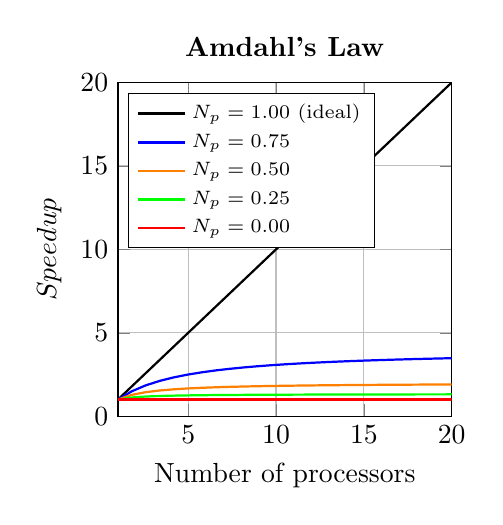
\begin{tikzpicture}
    \begin{axis}[
      xlabel={Number of processors},
      ylabel={$Speedup$},
      title=\textbf{Amdahl's Law},
      grid=major,
      xmin=1, xmax=20,
      ymin=0, ymax=20,
      height=0.48\textwidth, width=0.48\textwidth,
      domain=1:20,
      legend pos=north west,
      legend style={font=\scriptsize},
      legend cell align={left},
    ]
    \addplot[black, thick] {1 / ((1.0 - 1.0) + (1.0 / x))};
    \addlegendentry{$N_p=1.00$ (ideal)};
    \addplot[blue, thick] {1 / ((1.0 - 0.75) + (0.75 / x))};
    \addlegendentry{$N_p=0.75$};
    \addplot[orange, thick] {1 / ((1.0 - 0.5) + (0.5 / x))};
    \addlegendentry{$N_p=0.50$};
    \addplot[green, thick] {1 / ((1.0 - 0.25) + (0.25 / x))};
    \addlegendentry{$N_p=0.25$};
    \addplot[red, thick] {1 / ((1.0 - 0.0) + (0.0 / x))};
    \addlegendentry{$N_p=0.00$};
    \end{axis}
  \end{tikzpicture}
  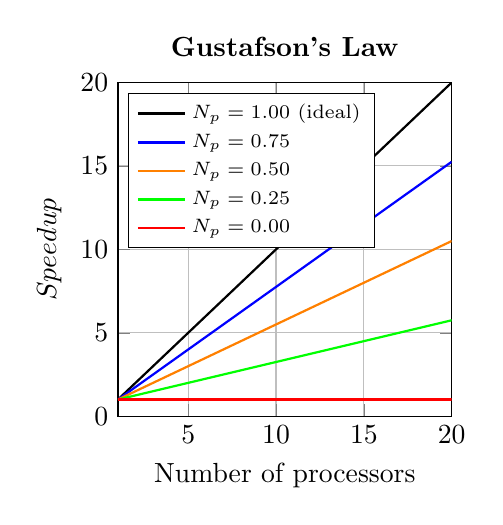
\begin{tikzpicture}
    \begin{axis}[
      xlabel={Number of processors},
      ylabel={$Speedup$},
      title=\textbf{Gustafson's Law},
      grid=major,
      xmin=1, xmax=20,
      ymin=0, ymax=20,
      height=0.48\textwidth, width=0.48\textwidth,
      domain=1:20,
      legend pos=north west,
      legend style={font=\scriptsize},
      legend cell align={left},
    ]
    \addplot[black, thick] {(1 - 1.0) + (1.0 * x)};
    \addlegendentry{$N_p=1.00$ (ideal)};
    \addplot[blue, thick] {(1 - 0.75) + (0.75 * x)};
    \addlegendentry{$N_p=0.75$};
    \addplot[orange, thick] {(1 - 0.5) + (0.5 * x)};
    \addlegendentry{$N_p=0.50$};
    \addplot[green, thick] {(1 - 0.25) + (0.25 * x)};
    \addlegendentry{$N_p=0.25$};
    \addplot[red, thick] {(1 - 0.0) + (0.0 * x)};
    \addlegendentry{$N_p=0.00$};
    \end{axis}
  \end{tikzpicture}
  \caption[Speedup according to Amdahl's and Gustafson's Laws]{\textbf{Speedup according to Amdahl's and Gustafson's Laws.} The speedup is presented as a function of the number of available processors for different fractions of parallelizable code ($N_p$), considering the estimates of Amdahl's and Gustafson's laws.}
  \label{fig:laws-plot}
\end{figure}

Following these rules, applications of parallel computing span various domains, from scientific simulations and data analytics to artificial intelligence. \ac{HPC} clusters address intricate scientific problems, such as simulating climate models, conducting molecular dynamics simulations for drug discovery, or analyzing large-scale genomics data. On the other hand, parallel processing significantly accelerates tasks like training machine learning models for image recognition, natural language processing, and recommendation systems. Additionally, parallel algorithms play a crucial role in speeding up tasks like sorting, searching, and graph traversal, contributing to improved efficiency in various computational domains. The future of parallel computing is influenced by ongoing advancements in hardware, software, and algorithms. Emerging technologies, such as quantum computing, introduce new dimensions to parallelism. Ongoing research explores novel ways to harness parallelism efficiently, overcome scalability challenges, and integrate parallel computing into mainstream applications. In summary, parallel computing stands as a cornerstone in addressing the escalating demands for computational power. Its comprehensive application ensures the development of efficient computational platforms for different research fields.

%%% Chapter 4: Data Coding in Structural Biology

\chapter{Data Coding in Structural Biology}

Data coding, in essence, refers to the process of representing information or data using a specific set of symbols, codes, or conventions. This encoding allows for the efficient storage, transmission, and processing of data. In computer science, data coding can involve various techniques, such as character encoding (representing characters with numerical values), binary coding (using combinations of 0s and 1s to represent information), and other methods tailored to specific types of data.

The data coding of biomolecules and binding sites plays a fundamental role in structural biology, enabling the computational representation, visualization and analysis of complex biological information \cite{kozlikova2016}. This process converts biological information into formats that are understandable and suitable for processing by algorithms and programs in computational systems. Data coding involves assigning numerical or categorical codes to biological components, \eg, atoms, amino acids, and nucleotides, to describe occupancy, coordinates, forces, physicochemical characteristics, and/or structural properties.

In structural biology, data coding is important for performing advanced analyses, \eg, molecular modeling, \ac{MD} simulations, and interaction prediction. There are several applications that exemplify the biological data coding for computational analyses. For instance, in molecular modeling, a protein can be coded using one-letter codes to represent different amino acids, as seen in protein sequence representation, to predict protein folding, as applied in ESMFold \cite{lin2022}, AlphaFold \cite{jumper2021} and RosettaFold \cite{baek2021}. In \acs{MD} simulation, the \acs{3D} coordinates of atoms or sets of atoms, along with vectors representing forces or other attributes, are used to represent the structure of a biomolecule, as in GROMACS \cite{gromacs} or AMBER \cite{amber} in atomistic-scale simulations and in CafeMol in coarse-grained molecular dynamics simulations \cite{kenzaki2011}. Additionally, binding sites, once identified by computational algorithms, are coded in different ways for further analyses. Binding sites can be coded to represent the spatial and physicochemical features of a biomolecular region, such as the \acs{3D} grids used in the KVFinder suite \cite{guerra2019,guerra2020,guerra2021,guerra2023B}, or the \acs{3D} coordinates of atoms, as in Fpocket \cite{fpocket}.

When working with computational models for the study of biomolecules, data coding is essential for the abstraction and computational representation of biological data. This abstraction is crucial for the development of computational tools aimed at studying biomolecular systems. Here, we present the data codings implemented for biomolecules and binding sites, \ie, volumetric representation, atomistic representation, and graph representation.

\section{Volumetric Representation}

Biomolecules and their binding sites can be represented in a \acs{3D} grid, organized into volumetric pixels, commonly known as voxels. This grid, akin to a matrix (\eg, a numpy array), assigns values to each voxel, encapsulating a discrete point of data within the \acs{3D} grid. Each voxel, acting as a discrete data point, can contain multiple types of information, enabling a straightforward and efficient representation of various properties within a specific portion of space (Figure \ref{fig:voxel}). In computer science, the \acs{3D} grid is a widely employed data structure in image processing and computer vision applications, including tasks such as image reconstruction, image segmentation, and object detection.

\begin{figure}[h]
  \centerline{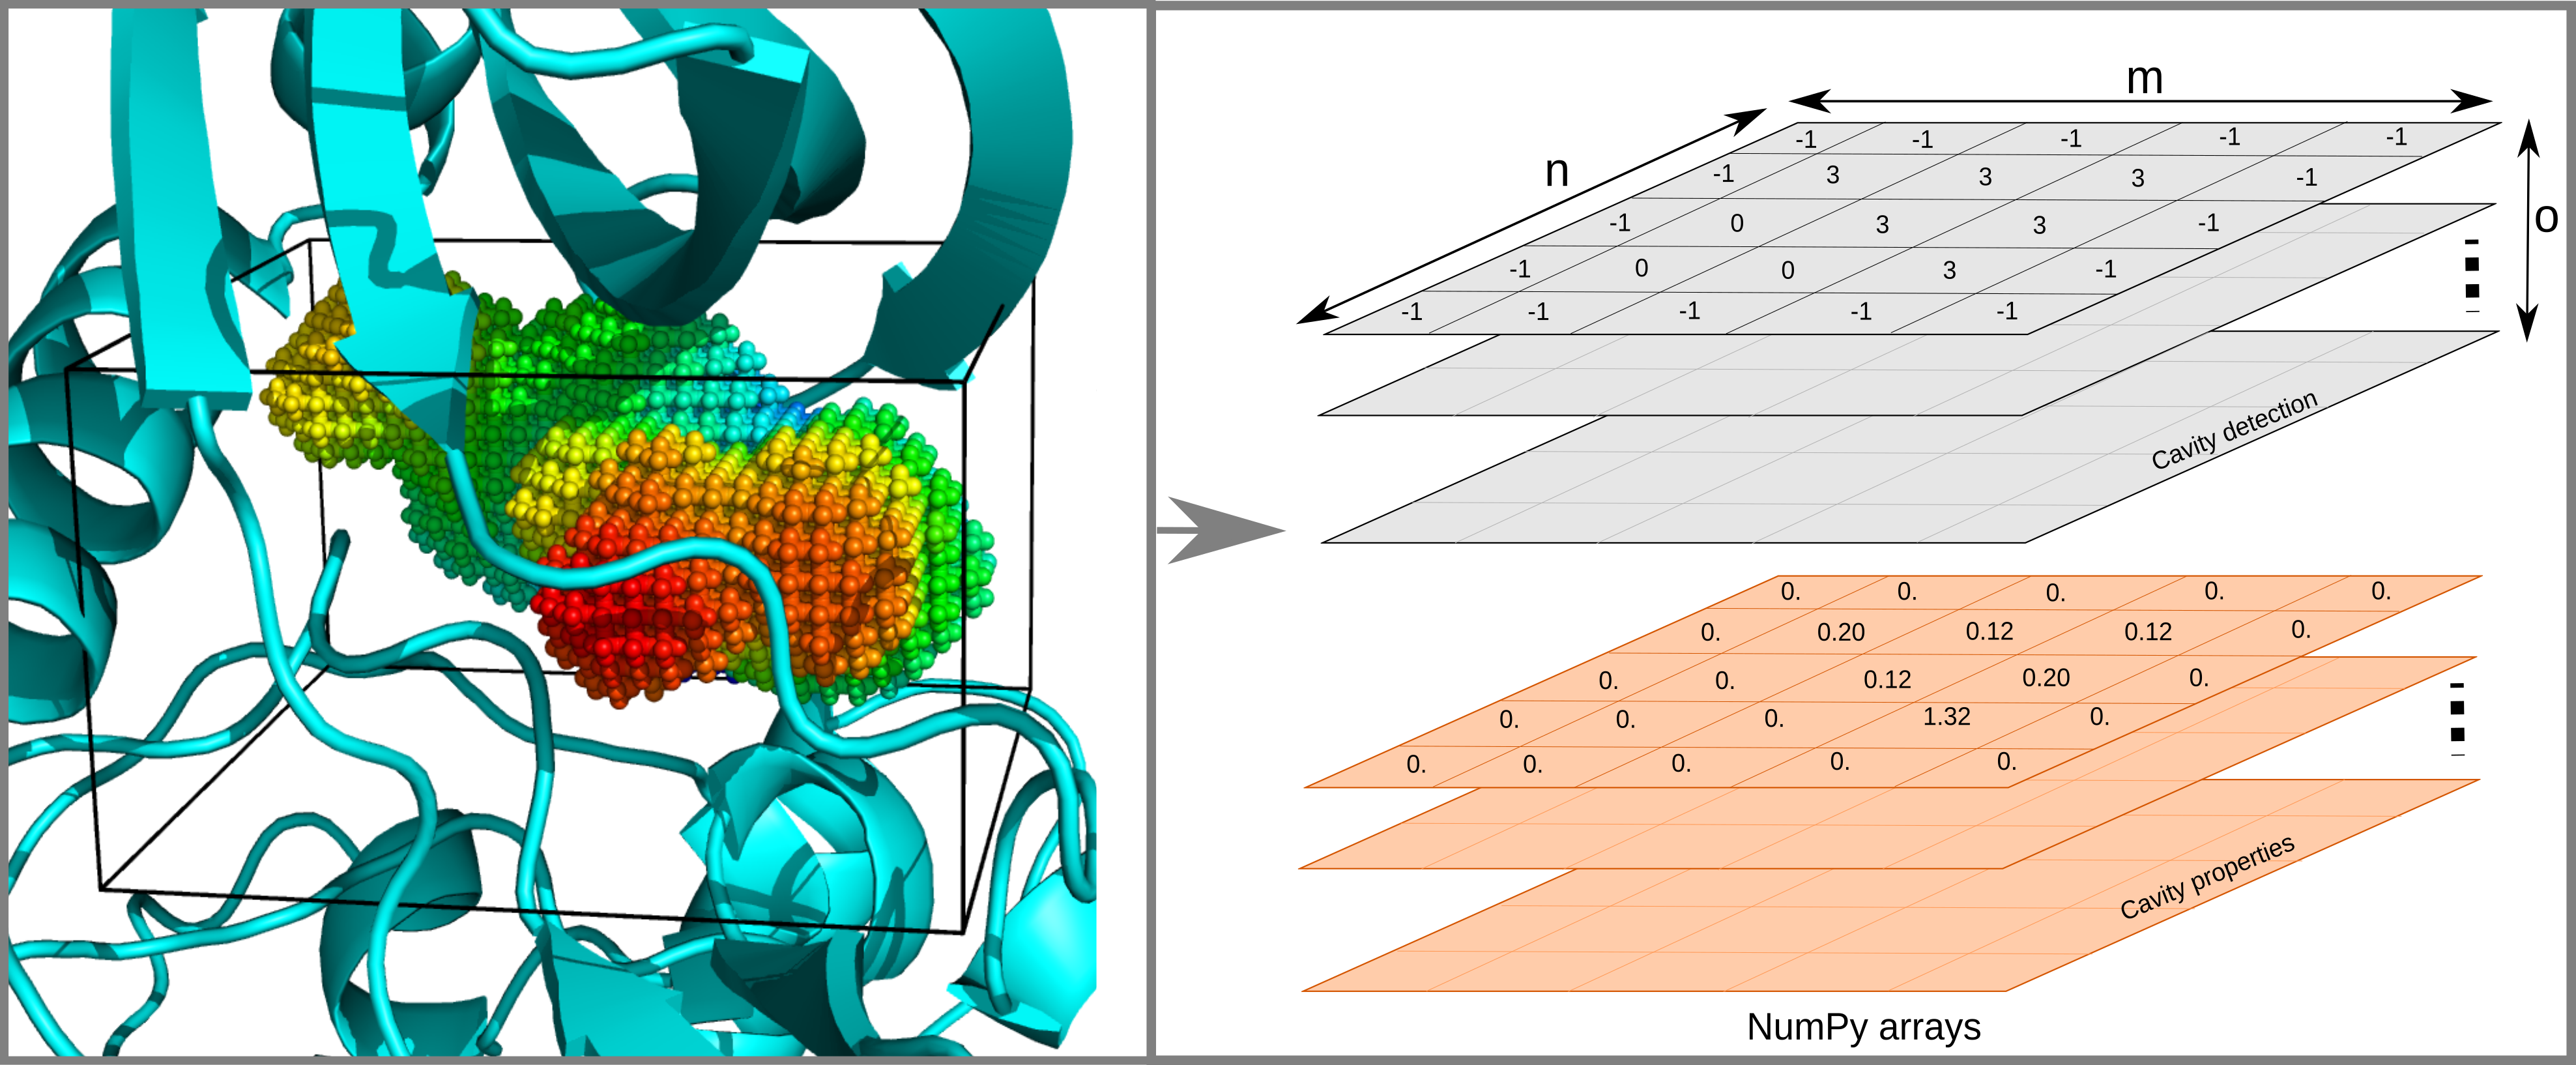
\includegraphics[scale=1]{images/voxels.png}}
  \centerline{\tiny{\textbf{Source:} Reprinted from \cite{guerra2021}. Licensed under \href{https://creativecommons.org/licenses/by/4.0/}{CC BY 4.0}.}}
  \caption[Grid representations]{\textbf{Grid representations.} Based on a 3D grid with dimensions (m, n, o), each element corresponds to a region of cavity (>1), empty space (1), biomolecule (0), or solvent (-1). Additionally, properties are stored in the same data structure, corresponding to the property value in the region.}
  \label{fig:voxel}
\end{figure}

Among various molecular surface representations, the \acs{3D} grid composed of voxels is the simplest and most suitable for representing multiple properties under various conditions, as each voxel in the \acs{3D} grid can store multiple information, \eg, charge distribution, burial extent (depth), hydrophobicity, hydrogen-bond-forming regions and cavity identifier. Moreover, the \acs{3D} grid is an efficient data structure for storing and accessing values and/or attributes at a \acs{3D} position, enabling the performance of mathematical and logical operations within a \acs{3D} region. Its versatility makes it an ideal choice for the development of computational algorithms, leveraging parallel computing techniques to accelerate the processing of large datasets.

The computational complexity of grid-based algorithms heavily relies on the input size, \ie, the number of voxels. Higher density grids offer a more detailed spatial representation, which proves beneficial for in-depth studies but comes at the cost of increased computational requirements, \ie, increased memory consumption and poorer time performance. For cavity detection algorithms, efficiency is often assessed based on the linear scalability of time complexity with the number of voxels, deeming exponential scalability inefficient. Within this context, the voxel clustering algorithm emerges as the most time-intensive step, primarily due to its limited parallelizability. 

In the parKVFiner software, the voxel length is a user-defined parameter, with default value of 0.6 Å. However, users have the flexibility to adjust this value based on the specific demands of their case studies. For instance, a smaller voxel length, such as 0.25 Å, is recommended for those seeking a more accurate morphological characterization of biomolecular cavities. The computational complexity is intricately tied to the number of voxels ($n_v$), denoted as $\mathcal{O}(n_v)$. User inputs determine the number of voxels (Eq. \ref{eq:nv}), calculated as follows:

\begin{equation}
  n_v \colon (l_x,l_y,l_z,Po,s) \mapsto \left \lceil \frac{l_x + 2 \cdot Po + s}{s} \right \rceil \cdot \left \lceil \frac{l_y + 2 \cdot Po + s}{s} \right \rceil \cdot \left \lceil \frac{l_z + 2 \cdot Po + s}{s} \right \rceil
  \label{eq:nv}
\end{equation}

\noindent where $l_x$, $l_y$, $l_z$ are the lengths of the target biomolecule along x, y, and z-axis, respectively, $Po$ is the \textit{Probe Out} size, $s$ is the grid spacing, and $\lceil \cdot \rceil$ is the ceiling function.

Under typical conditions, the average dimensions of the \acs{3D} grid, denoted as $(\bar{m},\bar{n},\bar{o})$, are roughly $(120,120,120)$, along the x, y, and z axes, respectively. The computational complexity increases as the region of interest, dictated by the biomolecule and the probe size, influences the number of voxels, where the voxel-level analysis, inherent to the algorithm, amplifies computational demands.

Turning to spatial complexity, the number of voxels and the bit-depth of grid elements significantly influence memory usage, with the latter also impacting precision. The choice between int (32-bit integer) and double (64-bit floating-point) in the C-coded parKVFinder reflects a balance between memory efficiency and the precision required for accurate calculations. Spatial complexity scales linearly with the number of voxels ($n_v$), denoted as $\mathcal{O}(n_v)$. In parKVFinder, the grid for cavity and surface points identifiers is an integer grid (32-bit integer), while cavity properties, such as point depth and hydrophobicity, are stored in a double grid (64-bit floating-point).

\subsection{Molecular Surface Representation}

The representation of molecular surfaces is a crucial step in the modeling and analysis of biomolecules. In this approach, biomolecules are described through a rigid sphere model, considering atomic positions and radii to represent the molecular surface. There are three commonly used mathematical formulations to represent molecular surfaces (Figure \ref{fig:surface-representation}):

\begin{enumerate}[label=\textbf{(\Alph*)}]
  \item \textbf{\acs{vdW} surface:} represents each atom as a sphere whose radius is proportional to its van der Waals radius. The \acs{vdW} surface is depicted as the union of these spherical atoms;
  \item \textbf{\acs{SAS}:} represents regions of a molecule that can be accessed by a solvent molecule (e.g., a water molecule), approximated by a spherical probe;
  \item \textbf{\acs{SES}:} is similar to \acs{SAS} but considers the outer shell of the probe instead of the probe's center.
\end{enumerate}
  
\begin{figure}[H]
  \centerline{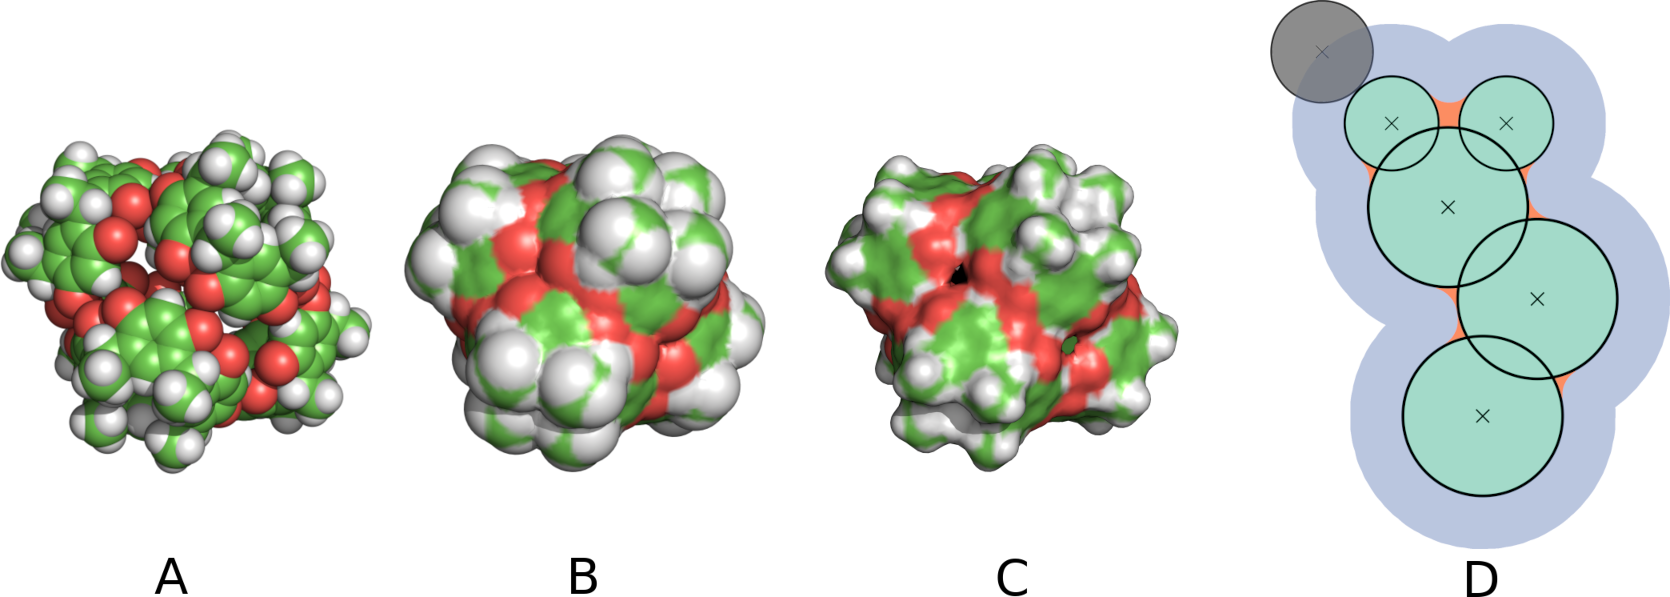
\includegraphics[scale=0.9]{images/surface-representation.png}}
  \centerline{\tiny{\textbf{Source:} Reprinted with permission from \cite{guerra2023B}. Copyright 2023 American Chemical Society.}}
  \caption[Molecular surface representations]{\textbf{Molecular surface representations.} \textbf{(A)} \acs{vdW} surface. \textbf{(B)} \acs{SAS}. \textbf{(C)} \acs{SES}. Images generated with PyMOL for the supramolecular cage (resorcin[4]arene-hexameric). \textbf{(D)} 2D schematic representation of molecular surfaces. The \acs{vdW} surface (green) consists of atoms represented as green spheres. A spherical probe (gray), representing a solvent molecule, rolls over the atoms of the molecule to define \acs{SES} and \acs{SAS}. \acs{SES} is defined by the \acs{vdW} surface (green) and the space not reached by the spherical probe (orange). \acs{SAS} is defined by the envelope reached by the center of the spherical probe (blue).}
  \label{fig:surface-representation}
\end{figure}

\section{Atomistic Representation}

In our exploration of structural and functional characterization, we now turn to atomistic representation, an alternative to the voxel-based approach. Rather than representing structural data through voxels in a \acs{3D} grid, biomolecules and their binding sites can also be portrayed through their atomistic representation (Figure \ref{fig:atomistic-representation}). This representations are applied in tools of molecular dynamics simulations, such as GROMACS \cite{gromacs}, AMBER \cite{amber}, and CafeMol \cite{kenzaki2011}. Here, atoms, residues, and/or nucleobases are modeled as hard sphere models in \acs{3D} coordinates (x, y, z), along with vectors (\eg, forces, velocities, and accelerations) and properties (\eg, mass, charge, and van der Waals radius).

\begin{figure}[h]
  \centerline{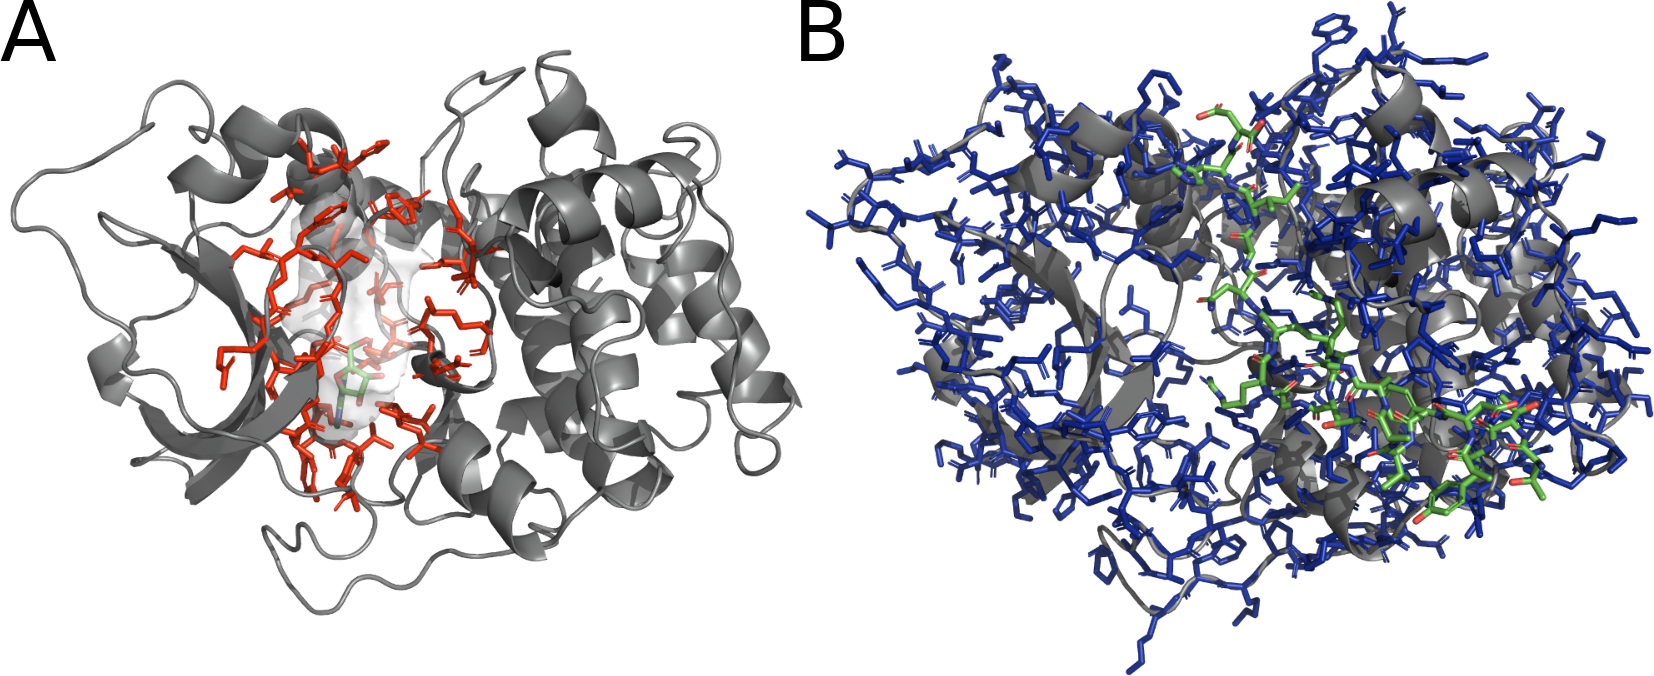
\includegraphics[scale=2]{images/atomistic-representation.png}}
  \caption[Atomistic representations]{\textbf{Atomistic representations.} \textbf{(A)} Atoms and amino acids (\textit{sticks} in green) forming the adenosine binding site (transparent surface). \textbf{(B)} Atoms and amino acids (\textit{sticks} in blue) exposed to the solvent, excluding binding sites for small molecules, with an inhibitor bound (\textit{sticks} in green). Images generated with PyMOL for a subunit of cyclic AMP-dependent protein kinase (PDB ID: 1FMO).}
  \label{fig:atomistic-representation}
\end{figure}

Yet, when delving effectively into interaction regions, a prerequisite emerges---the filtration of areas of interest, such as binding sites (Figure \ref{fig:atomistic-representation}A) or solvent-exposed regions (Figure \ref{fig:atomistic-representation}B). This atomistic representation allows precise and in-depth analysis, focusing on interactions and structural features relevant to biological function. Additionally, atomistic information can be utilized in molecular docking studies, rational drug design, and prediction of molecular interactions. These applications significantly contribute to the development of new therapeutic compounds and aid in understanding the molecular mechanisms involved in biological processes.

Parallel to the challenges encountered in volumetric representation, the computational complexity of algorithms based on atomistic representations hinges on the input size---specifically, the number of atoms. Researchers must balance the level of detail required for their analyses with the computational resources available, opting for fine-grained (all-atom), coarse-grained or carbon\textalpha\space (backbone) models. Spatial complexity is linearly dependent on the number of atoms ($n_a$), denoted as $\mathcal{O}(n_a)$. 

Within parKVFinder, the atomistic representation encodes each atom by its residue number (32-bit integer), chain identifier (char), residue name (4-char array), atom type (char), coordinates (64-bit floating-point), and \acs{vdW} radius (64-bit floating-point). Concurrently, interface residues are represented by residue number (32-bit integer), chain identifier (char) and residue name (4-char array). In both instances, spatial complexity significantly diminishes compared to volumetric representation, given the fewer atoms or interface residues compared to voxels for the same target biomolecule. When applying atomistic representation, researchers adopt the biomolecule's perspective, in contrast to the cavity point-of-view inherent in volumetric representation.

\section{Graph Representation \label{sec:graph-representation}}

Expanding upon the atomistic representation, the utilization of graph-based models emerges as a robust representation for examining interactions and relationships within biomolecules. Graph theory techniques are widely applied across diverse scientific domains such as biology, chemistry, physics, computer science, and mathematics \cite{foulds1995, majeed2020}. A cornerstone in discrete mathematics, it models the relationships and interactions between objects in a network, assisting in the analysis of biological interaction networks at various scales. In structural biology, graph theory has been utilized to investigate the structure, folding, stability, function, allostery and dynamics of proteins \cite{vishveshwara2002,dipaola2015,heal2018,kantelis2022}.

A graph $\mathcal{G(V,E)}$ (Figure \ref{fig:graph-examples}) is a mathematical structure, where $\mathcal{V} = \{v_1, v_2, \dots, v_n\}$ is a nonempty, finite set of vertices (also known nodes, point and junction), and $\mathcal{E} = \{e_1, e_2, \dots, e_n\}$ is a set of unordered pairs of distinct vertices of $\mathcal{V}$, whose elements $\{v_i,v_j\} \in \mathcal{E}$, where $v_i,v_j \in \mathcal{V}$, connects vertices $v_i$ and $v_j$ and termed edges (also known as line, arc, branch and link). Graphs can be directed (also known as digraph), where edges link two vertices symmetrically, or undirected, where edges link two vertices asymmetrically. Additionally, graphs can also be weighted, where each edge is assigned a weight or cost, which can represent a physical distance, a similarity measure, or any other property \cite{foulds1995,bondy1976,majeed2020,black2020}. Evolving from this, graph theory finds applications in modeling biological and chemical systems. In chemistry, molecular graphs capture the structural relationships between atoms and bonds, facilitating the study of chemical compounds and reactions. Biomolecules, which are assemblies of atoms (vertices) connected by intramolecular and intermolecular interactions (edges), have also been extensively explored through graph theory \cite{vishveshwara2002,mason2007}.

\begin{figure}[h]
  \centering
  \begin{subfigure}{0.32\textwidth}
    \centering
    \textbf{\footnotesize{Undirected graph}}
    \vspace{0.25cm} \\
    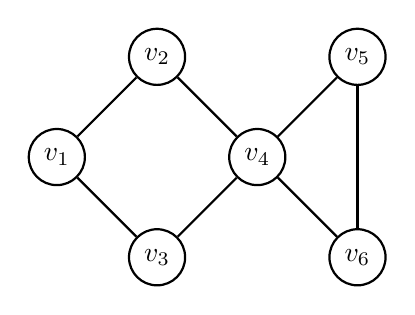
\begin{tikzpicture}[node distance={18mm}, thick]
      \node[ConnNode] (1) {$v_1$}; 
      \node[ConnNode] (2) [above right of=1] {$v_2$}; 
      \node[ConnNode] (3) [below right of=1] {$v_3$}; 
      \node[ConnNode] (4) [above right of=3] {$v_4$}; 
      \node[ConnNode] (5) [above right of=4] {$v_5$}; 
      \node[ConnNode] (6) [below right of=4] {$v_6$}; 
      \draw (1) -- (2); 
      \draw (1) -- (3); 
      \draw (2) -- (4); 
      \draw (3) -- (4);
      \draw (4) -- (5);
      \draw (4) -- (6);
      \draw (5) -- (6);
    \end{tikzpicture}
  \end{subfigure}
  \hfill
  \begin{subfigure}{0.32\textwidth}
    \centering
    \textbf{\footnotesize{Directed graph}}
    \vspace{0.25cm} \\
    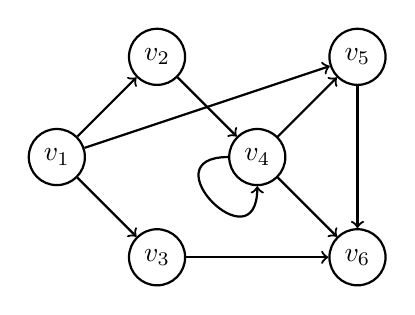
\begin{tikzpicture}[node distance={18mm}, thick]
      \node[ConnNode] (1) {$v_1$}; 
      \node[ConnNode] (2) [above right of=1] {$v_2$}; 
      \node[ConnNode] (3) [below right of=1] {$v_3$}; 
      \node[ConnNode] (4) [above right of=3] {$v_4$}; 
      \node[ConnNode] (5) [above right of=4] {$v_5$}; 
      \node[ConnNode] (6) [below right of=4] {$v_6$};
      \draw[->] (1) -- (2); 
      \draw[->] (1) -- (3);
      \draw[->] (1) -- (5); 
      \draw[->] (2) -- (4); 
      \draw[->] (3) -- (6);
      \draw[->] (4) to [out=180,in=270,looseness=5] (4); 
      \draw[->] (4) -- (5);
      \draw[->] (4) -- (6);
      \draw[->] (5) -- (6);
    \end{tikzpicture}
  \end{subfigure}
  \hfill
  \begin{subfigure}{0.32\textwidth}
    \centering
    \textbf{\footnotesize{Weighted graph}}
    \vspace{0.25cm} \\
    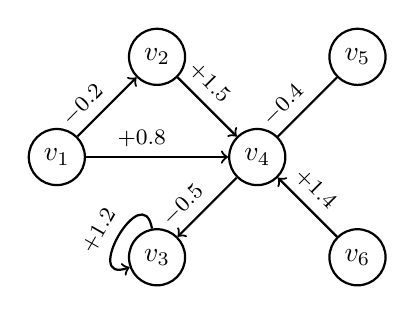
\begin{tikzpicture}[node distance={18mm}, thick]
      \node[ConnNode] (1) {$v_1$}; 
      \node[ConnNode] (2) [above right of=1] {$v_2$}; 
      \node[ConnNode] (3) [below right of=1] {$v_3$};
      \node[circle] (Aux3) [above left=0.2cm and 0cm of 3, rotate=60] {\footnotesize{$+1.2$}}; 
      \node[ConnNode] (4) [above right of=3] {$v_4$}; 
      \node[ConnNode] (5) [above right of=4] {$v_5$}; 
      \node[ConnNode] (6) [below right of=4] {$v_6$};
      \draw[->] (1) -- node[midway, above right, sloped, pos=-0.1] {\footnotesize{$-0.2$}} (2);
      \draw[->] (1) -- node[midway, above right, sloped, pos=0.15] {\footnotesize{$+0.8$}} (4);
      \draw[->] (2) -- node[midway, above right, sloped, pos=-0.1] {\footnotesize{$+1.5$}} (4);
      \draw[->] (3) to [out=100,in=200,looseness=3] (3); 
      \draw[->] (4) -- node[midway, above right, sloped, pos=1.1] {\footnotesize{$-0.5$}} (3);
      \draw (5) -- node[midway, above right, sloped, pos=1.1] {\footnotesize{$-0.4$}} (4);
      \draw[->] (6) -- node[midway, above right, sloped, pos=1] {\footnotesize{$+1.4$}} (4); 
    \end{tikzpicture}
  \end{subfigure}
  \caption[Pictorial overview of graphs $\mathcal{G(V,E)}$]{\textbf{Pictorial overview of graphs $\mathcal{G(V,E)}$.}}
  \label{fig:graph-examples}
\end{figure}

In this context, we introduce a graph-based representation for biomolecules using the \acs{3D} coordinates (x, y, z) of a biomolecular structure or complex that generates a residue-level graph, where vertices represent residues and edges represent interactions or some type of relationship between them. The construction of edges is based on customizable distance cutoffs between atoms, such as \ac{CA}, \ac{CB}, or any other atom, which can be defined by the user (Figure \ref{fig:graph-representation}). According to \ac{CAPRI} Round 28 \cite{capri,round28}, a distance cutoff of 8 Å between any two \acs{CB} atoms (or \acs{CA} for Gly) define interface residues, and a distance cutoff of 4 Å between any two atoms define native contacts. Expanding on the \acs{CB} definition, a distance cutoff of 10 Å between any two \acs{CA} atoms to define interface residues. Thus, the default parameters set in the implementation are these distance cutoffs, establishing relationships or interactions between residues \cite{vishveshwara2002,mason2007}. Figure \ref{fig:graph-representation}A shows an example of a residue-level graph generated from an adenosine binding site (Figure \ref{fig:atomistic-representation}A), and Figure \ref{fig:graph-representation}B shows an example of a residue-level graph generated from a solvent-exposed surface (Figure \ref{fig:atomistic-representation}B).

\begin{figure}[H]
\centerline{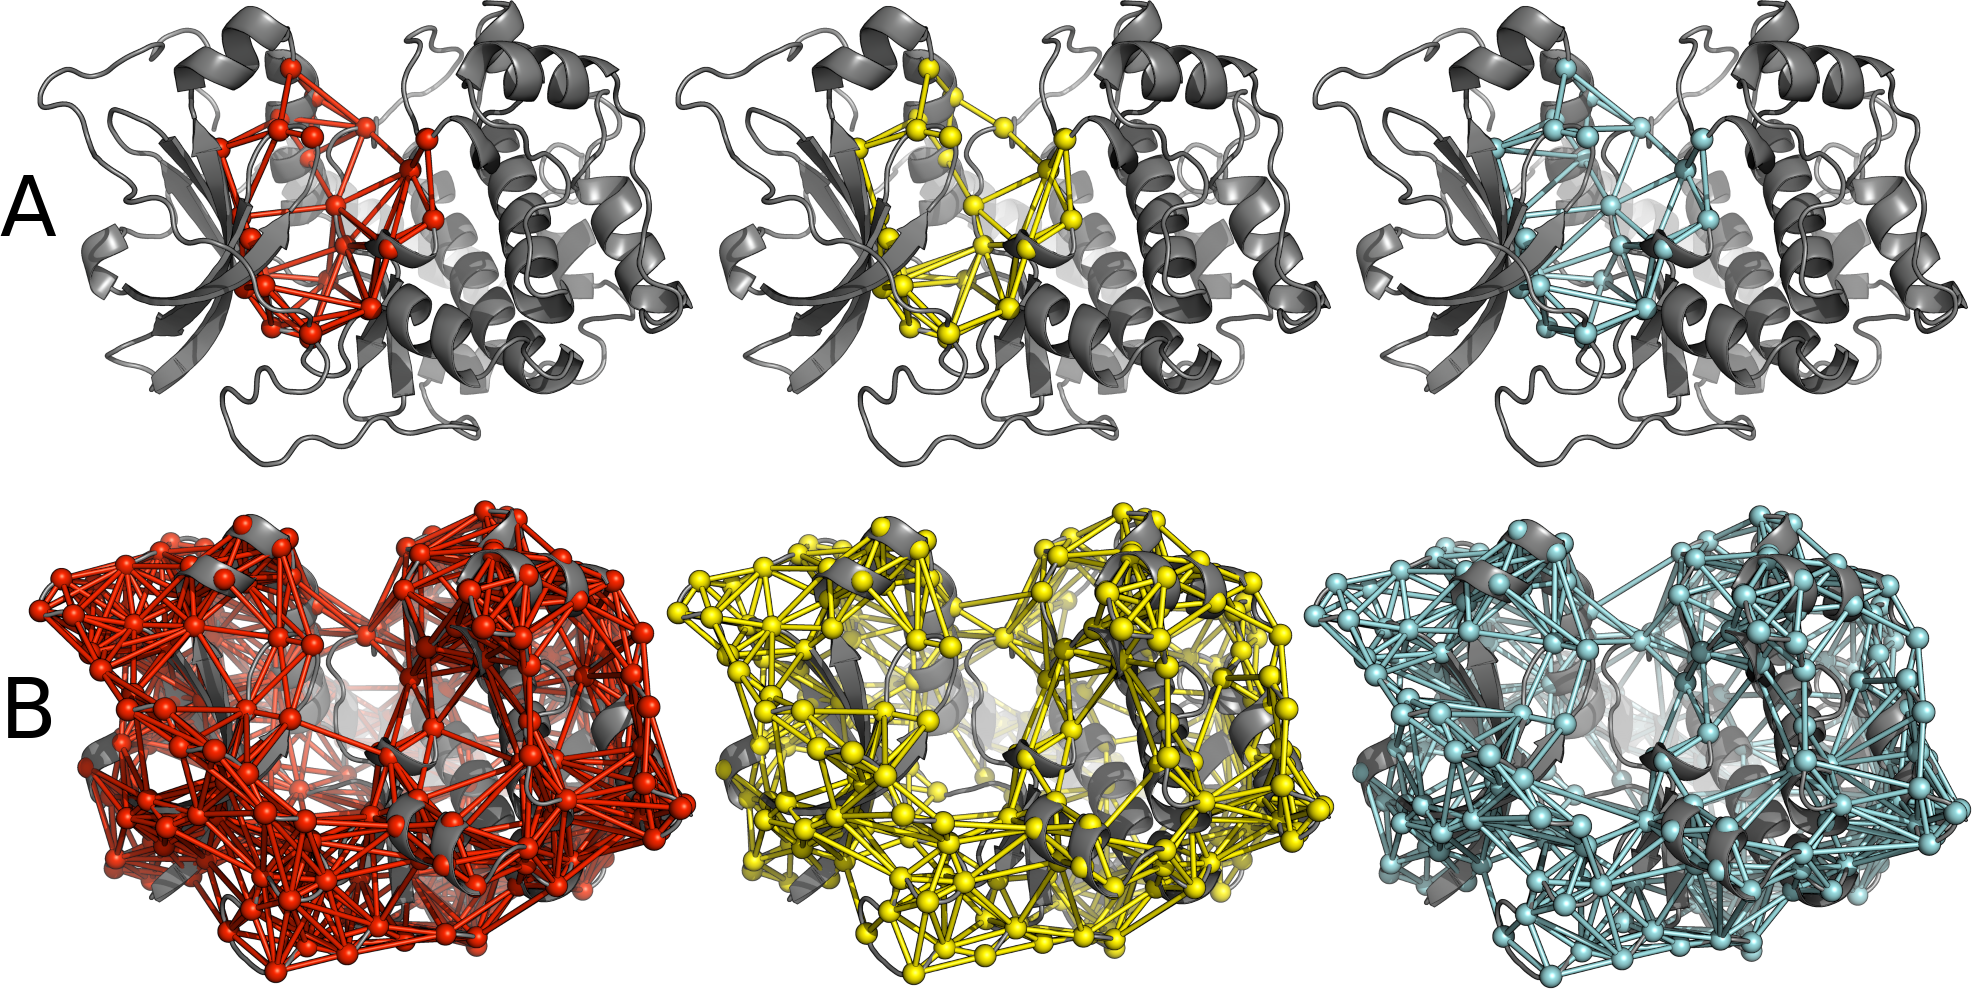
\includegraphics[scale=1.5]{images/graph-representation.png}}
\caption[Graph representations]{\textbf{Graph representations.} \textbf{(A)} Adenosine binding site as graphs with edges based on the distance cutoff of \acs{CA} (spheres and sticks in red), \acs{CB} (spheres and sticks in yellow), and any atoms of the residues (spheres and sticks in cyan). \textbf{(B)} Solvent-exposed surface, excluding binding sites for small molecules, as graphs with edges based on the distance cutoff of \acs{CA} (spheres and sticks in red), \acs{CB} (spheres and sticks in yellow), and any atoms of the residues (spheres and sticks in cyan). Images generated with PyMOL for a subunit of cyclic AMP-dependent protein kinase (PDB ID: 1FMO).}
\label{fig:graph-representation}
\end{figure}

This graph-based representation allows a more efficient analysis of interactions and relationships between residues, providing a visually intuitive exploration of the structural and functional attributes of the biomolecule. Additionally, various properties and metrics can be calculated from the graphs, such as paths, distances, centrality, and other metrics that aid in understanding the structure and function of the biomolecule \cite{majeed2020,vishveshwara2002,mason2007}. Since our primary focus is on the adjacency matrix, spatial complexity depends on the square of the number of vertices (\ie, number of residues---$n_r$), denoted as $\mathcal{O}(n_{r}^{2})$. However, as we include attributes (weights) on vertices and edges, spatial complexity will depend on the size of this additional data. With this graph-based representation in hand, novel mathematical approaches from graph theory can be applied to deepen our understanding of biological function and provide crucial insights for the development of therapies and therapeutic interventions.

%%% Chapter 5: KVFinder suite

% https://cnpemcamp-my.sharepoint.com/:w:/r/personal/joao_guerra_lnbio_cnpem_br/_layouts/15/Doc.aspx?sourcedoc=%7BD0C80180-AF7E-412F-B94E-6C38D8D4C946%7D&file=Relat%C3%B3rio%20Plataforma%20Biologia%20Computacional%202022.2.docx&action=default&mobileredirect=true


\chapter{KVFinder suite \label{ch:kvfinder-suite}}

The interactions between biomolecules play a crucial role in biological processes, involving entities ranging from small molecules such as ions and drugs to macromolecules such as proteins and nucleic acids. These receptor-ligand interactions (\eg, IPPs, IPLs, IPRs, and IPDs) take place at specific binding sites, which can be solvent-exposed clefts or cavities buried within the receptors. Morphological, topological, and physicochemical complementarity between ligands and receptors governs molecular recognition, limiting efficient interaction to a finite number of ligands. The identification and assessment of these regions are fundamental for understanding the tertiary structure of biomolecules and for the development of new drugs. To meet this demand, we have developed the computational platform \textbf{KVFinder suite}, which combines precise tools with high-performance processing, enabling the analysis of biomolecular experimental data and the comprehension of the biomolecular structure and function in biological systems.

The KVFinder suite consists of five computational tools that offer comprehensive functionalities for structural analysis and the study of biomolecular interactions. The tools included in the platform are: parKVFinder \cite{guerra2019,guerra2020}, pyKVFinder \cite{guerra2021}, KVFinder-web \cite{guerra2023A}, SERD, and KVFinderMD. Below, we will describe each of these tools, their main features, and their guideline applications.

\section{parKVFinder \label{sec:parkvfinder}}

The \ac{parKVFinder} \cite{guerra2020} is an open-source tool, licensed under GPL v3.0, developed for the detection and characterization of any type of biomolecular cavity. Originating from the master's thesis entitled "Prospecção e caracterização de cavidades supramoleculares" \cite{guerra2019}, it presents itself as an refactored, optimized and parallelized successor of KVFinder \cite{oliveira2014}. The initial release, \href{https://github.com/LBC-LNBio/parKVFinder/tree/v1.0}{parKVFinder v1.0}, was published in SoftwareX \cite{guerra2020}, with morphological (\ie, shape, volume, and area) and constitutional (\ie, interface residues surrounding cavities) characterizations. Progressing further, \href{https://github.com/LBC-LNBio/parKVFinder/tree/v1.0}{parKVFinder v1.0} was published in SoftwareX \cite{guerra2020}, with morphological (\ie, shape, volume, and area) and constitutional (\ie, interface residues surrounding cavities) characterizations. A notable addition was a novel algorithm for surface area estimation, based on Mullikin & Verbeek voxel classification. Progressing further, \href{https://github.com/LBC-LNBio/parKVFinder/tree/v1.2.0}{parKVFinder v1.2.0} expanded its capabilities with additional morphological (\ie, depth), physicochemical (\ie, Eisenberg & Weiss hydrophobicity \cite{eisenberg1984}), and constitutional (\ie, residue frequency) characterizations \cite{guerra2023A}. 

The parKVFinder software is integrated with the PyMOL molecular viewer \cite{pymol} through a graphical plugin. The original plugin, PyMOL parKVFinder Tools, was developed for PyMOL v1.8 \cite{guerra2019,guerra2020}. However, with the advent of PyMOL v2.0 by Schröndinger, which discontinued support for the 1.8 version, a new plugin was developed---PyMOL2 parKVFinder Tools (Figure \ref{fig:pymol2-parkvfinder-tools}), written in Python3 with Qt interface. This update plugin incorporates new characterizations (depth and Eisenberg & Weiss hydrophobicity) from parKVFinder v1.2.0. This new plugin provides an intuitive and easy-to-use \ac{GUI}, allowing users to customize parameters for the detection and characterization of cavities.  Additionally, users can visualize identified cavities and their characteristics directly within the PyMOL environment (Figure \ref{fig:pymol2-parkvfinder-tools-visualization}). Alongside the \acs{GUI}, parKVFinder also serves advanced users with a \ac{CLI}, enabling task automation and program integration. The source code for parKVFinder and the PyMOL plugins is publicly available in the following repository: \url{https://github.com/LBC-LNBio/parKVFinder}.

\begin{figure}
  \centering
  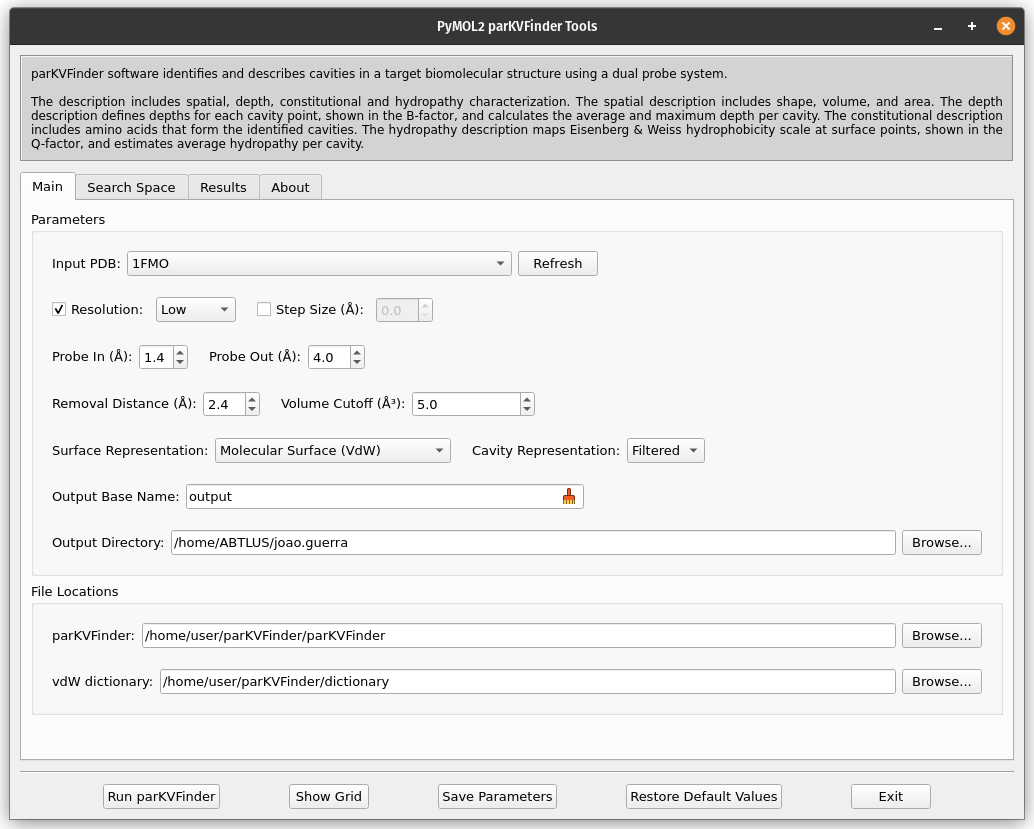
\includegraphics[scale=0.35]{images/pymol2-parkvfinder-tools.png}
  \caption[PyMOL2 parKVFinder Tools]{\textbf{PyMOL2 parKVFinder Tools.} The \textit{Main} tab presents the options that directly control the cavity detection procedure, in which user can set \textit{Probe In} and \textit{Probe Out} sizes, grid spacing, removal distance, volume filter, surface representation and cavity representation. Space segmentation features are managed in the \textit{Search Space} tab, allowing users to designate either the entire structure or custom search spaces. In box adjustment mode, an interactive box is drawn in the PyMOL viewer. Additionally, users can opt for ligand adjustment, limiting the search space around a defined ligand (PyMOL object) to a user-specified radius. After running parKVFinder, results (volume, surface area, depth, hydropathy, and interface residues) are interactively accessible in the \textit{Results} tab, and the cavity PDB file seamlessly loads into the PyMOL viewer.}
  \label{fig:pymol2-parkvfinder-tools}
\end{figure}

\begin{figure}[ht]
  \centering
  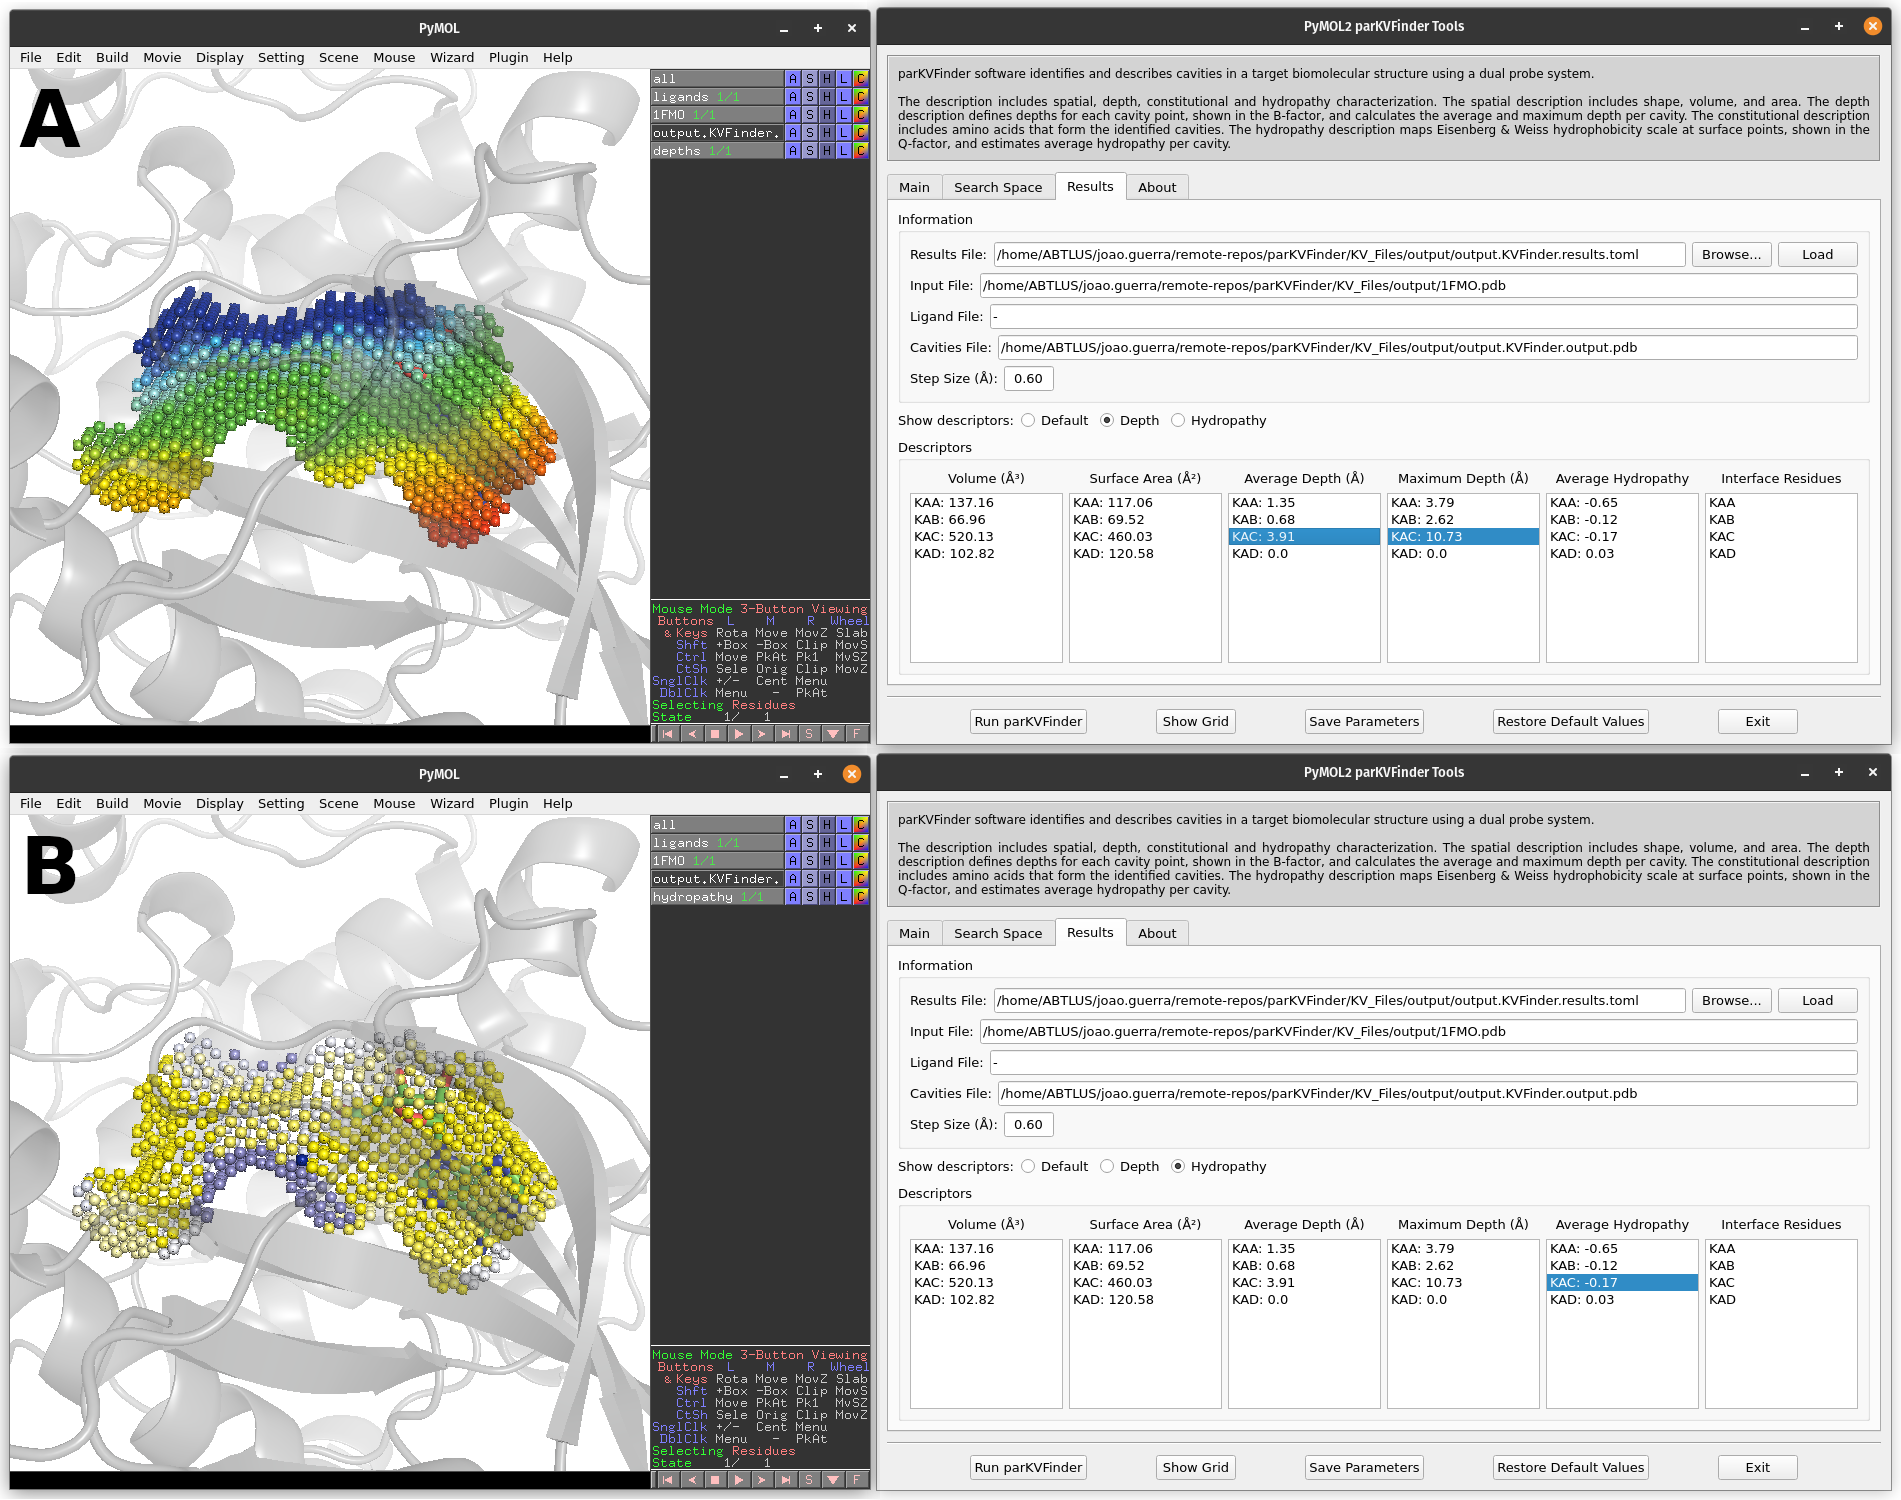
\includegraphics[scale=1]{images/pymol2-parkvfinder-tools-visualization.png}
  \caption[Interactive view of PyMOL2 parKVFinder Tools in PyMOL]{\textbf{Interactive view of PyMOL2 parKVFinder Tools in PyMOL.} Cavity characterization of the adenosine binding site in a protein kinase A (PDB ID: 1FMO). \textbf{(A)} Depth characterization: cavity points are colored by depth, ranging from superficial (blue points) to buried (red points). \textbf{(B)} Hydropathy characterization: surface cavity points are colored by Eisenberg & Weiss hydrophobicity scale, from $-1.42$ (highly hydrophobic) to $2.6$ (highly hydrophilic).}
  \label{fig:pymol2-parkvfinder-tools-visualization}
\end{figure}

Cavity detection and characterization routines in parKVFinder leverage the OpenMP library for parallelization, optimizing performance on multicore systems. Computational assessments on a set of 1000 protein domains (kv1000, \url{https://github.com/jvsguerra/kv1000}) revealed significant runtime reductions compared to KVFinder. The code optimization yielded a speedup of $\sim$1.5 times \cite{guerra2019} compared to KVFinder, and the subsequent code parallelization in parKVFinder led to a speedup of $\sim$6.5 times \cite{guerra2020}. Overall, parKVFinder demonstrated a remarkable $\sim$9.5 times reduction in runtime compared to KVFinder \cite{guerra2019,guerra2020}.

\subsection{Case Studies}

The parKVFinder software has been applied in two case studies published in scientific journals to investigate proteins of therapeutic interest. These analyses explored the dynamics of the flaps of the \ac{HIV-1} protease \cite{guerra2020} and the hydrophobicity profile of binding sites in alphaviruses \cite{ribeiro2021}. Below, we will describe each of these case studies in detail.

\subsection{Molecular Dynamics of HIV-1 Protease \label{sec:md-hiv1-protease}}

The active site of the HIV-1 protease represents a relevant therapeutic target for various antiretroviral drugs. This binding site exhibits significant complexity, which arises from the movement of \textbeta-hairpins, known as flaps, leading to structural and morphological variations. The volume of the binding site changes with the motion of these flaps, influencing substrate accessibility to the active site of the homodimer \cite{lam1994,soares2016}.

In this study, the \acs{MD} of the HIV-1 protease was investigated by identifying and evaluating the active site's volume during \acs{MD} simulations. Our objective was to describe the dynamic movement of the flaps through the volume and shape of the active site cavity as conformational descriptors in \acs{MD} simulations. To achieve this, 200 ns \acs{MD} simulations were conducted using the GROMACS 2019.4 package \cite{gromacs}, the AMBER99SB-ws force field, and the TIP42005s water model. The simulations initiated from the crystallographic structure of HIV-1 protease in the closed conformation \cite{lam1994}, excluding the inhibitor present in the structure, cyclic urea.

\begin{figure}[h]
  \centerline{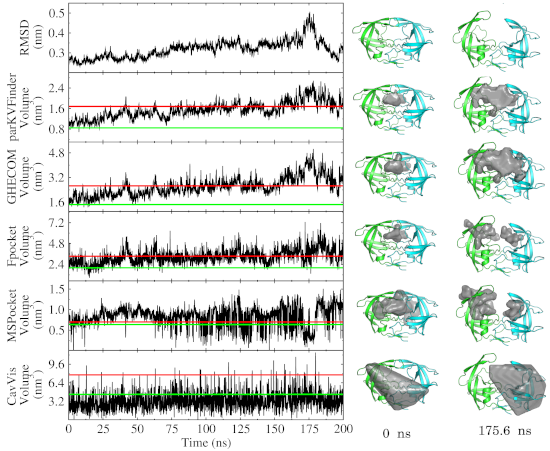
\includegraphics[scale=1.2]{images/hiv1-protease-md-analysis.png}}
  \centerline{\tiny{\textbf{Source:} Reprinted from \cite{guerra2020}. Licensed under \href{https://creativecommons.org/licenses/by/4.0/}{CC BY 4.0}.}}
  \caption[Volume of the HIV-1 protease active site over a 200 ns molecular dynamics simulation]{\textbf{Volume of the HIV-1 protease active site over a 200 ns molecular dynamics simulation.} The green and red lines indicate the cavity volume for the closed (PDB ID: 1HVR) and semi-open (PDB ID: 1HHP) states, respectively. Protein structures at the beginning of the simulation (0 ns) and the frame with the highest \acs{RMSD} (175.6 ns) are shown as cartoons. The corresponding cavities detected by each tool are displayed as gray surfaces.}
  \label{fig:hiv1-protease-dm-analysis}
\end{figure}

The active site volume was monitored throughout the \acs{MD} simulations (Figure \ref{fig:hiv1-protease-dm-analysis}). Initially, the cavity volume corresponds to the closed conformation (green line). After $\sim$25 ns, it increases, reaching the value corresponding to the semi-open conformation (red line) around 75 ns, indicating an opening process. Subsequently, the flaps separate further, and the cavity achieves its maximum volume at $\sim$175 ns before reverting to the more stable semi-open conformation. This dynamic volume change correlates well (Pearson correlation; $\rho=0.72$) with the \ac{RMSD} of the \acs{CA} calculated from the closed conformation, providing an accurate depiction of the protein's conformational state throughout the simulation. It is noteworthy that \acs{RMSD} describes global structural variations, while the estimated volume offers a direct metric of conformational changes in the active site, possibly associated with ligand accessibility.

The performance of parKVFinder \cite{guerra2020} was benchmarked against other geometry-based methods (Figure \ref{fig:hiv1-protease-dm-analysis}), including GHECOM \cite{ghecom}, Fpocket \cite{fpocket}, MSPocket \cite{mspocket}, and CavVis \cite{cavvis}. The correlation between the estimated volume by each program and the \acs{RMSD} was evaluated, replicating the approach used for parKVFinder. The volume estimated by GHECOM ($\rho=0.75$) correlates with the conformational state, similar to parKVFinder ($\rho=0.72$), likely due to their shared use of grid-and-sphere-based methods. However, the cavities identified by Fpocket ($\rho=0.35$), MSPocket ($\rho=-0.24$), and CavVis ($\rho=0.19$) did not show a satisfactory correlation with the conformational dynamics of the active site. Therefore, parKVFinder and GHECOM demonstrated high accuracy in describing the conformational state of the HIV-1 protease active site.

Beyond accuracy, the computational time of the programs was also assessed (Figure \ref{fig:hiv1-protease-dm-times}). parKVFinder ($t=1h03m$) was at least four times faster than GHECOM ($t=4h32m$), due to the multi-threaded subroutines implemented in parKVFinder. Furthermore, parKVFinder outperformed MSPocket ($t=2h48m$) and CavVis ($t=3h45$) in terms of computational time but did not surpass Fpocket ($t=20m$), which uses Voronoi tessellation and \textalpha\space spheres methods, resulting in fast computations. However, this implementation of Fpocket proved less sensitive in the detailed description of the HIV-1 protease active site, inefficiently distinguishing the conformational states of the active site. Therefore, considering accuracy and performance, parKVFinder emerged as a robust option for the spatial detection and characterization of cavities in the case study of the HIV-1 protease \cite{guerra2020}.

\begin{figure}[H]
  \centerline{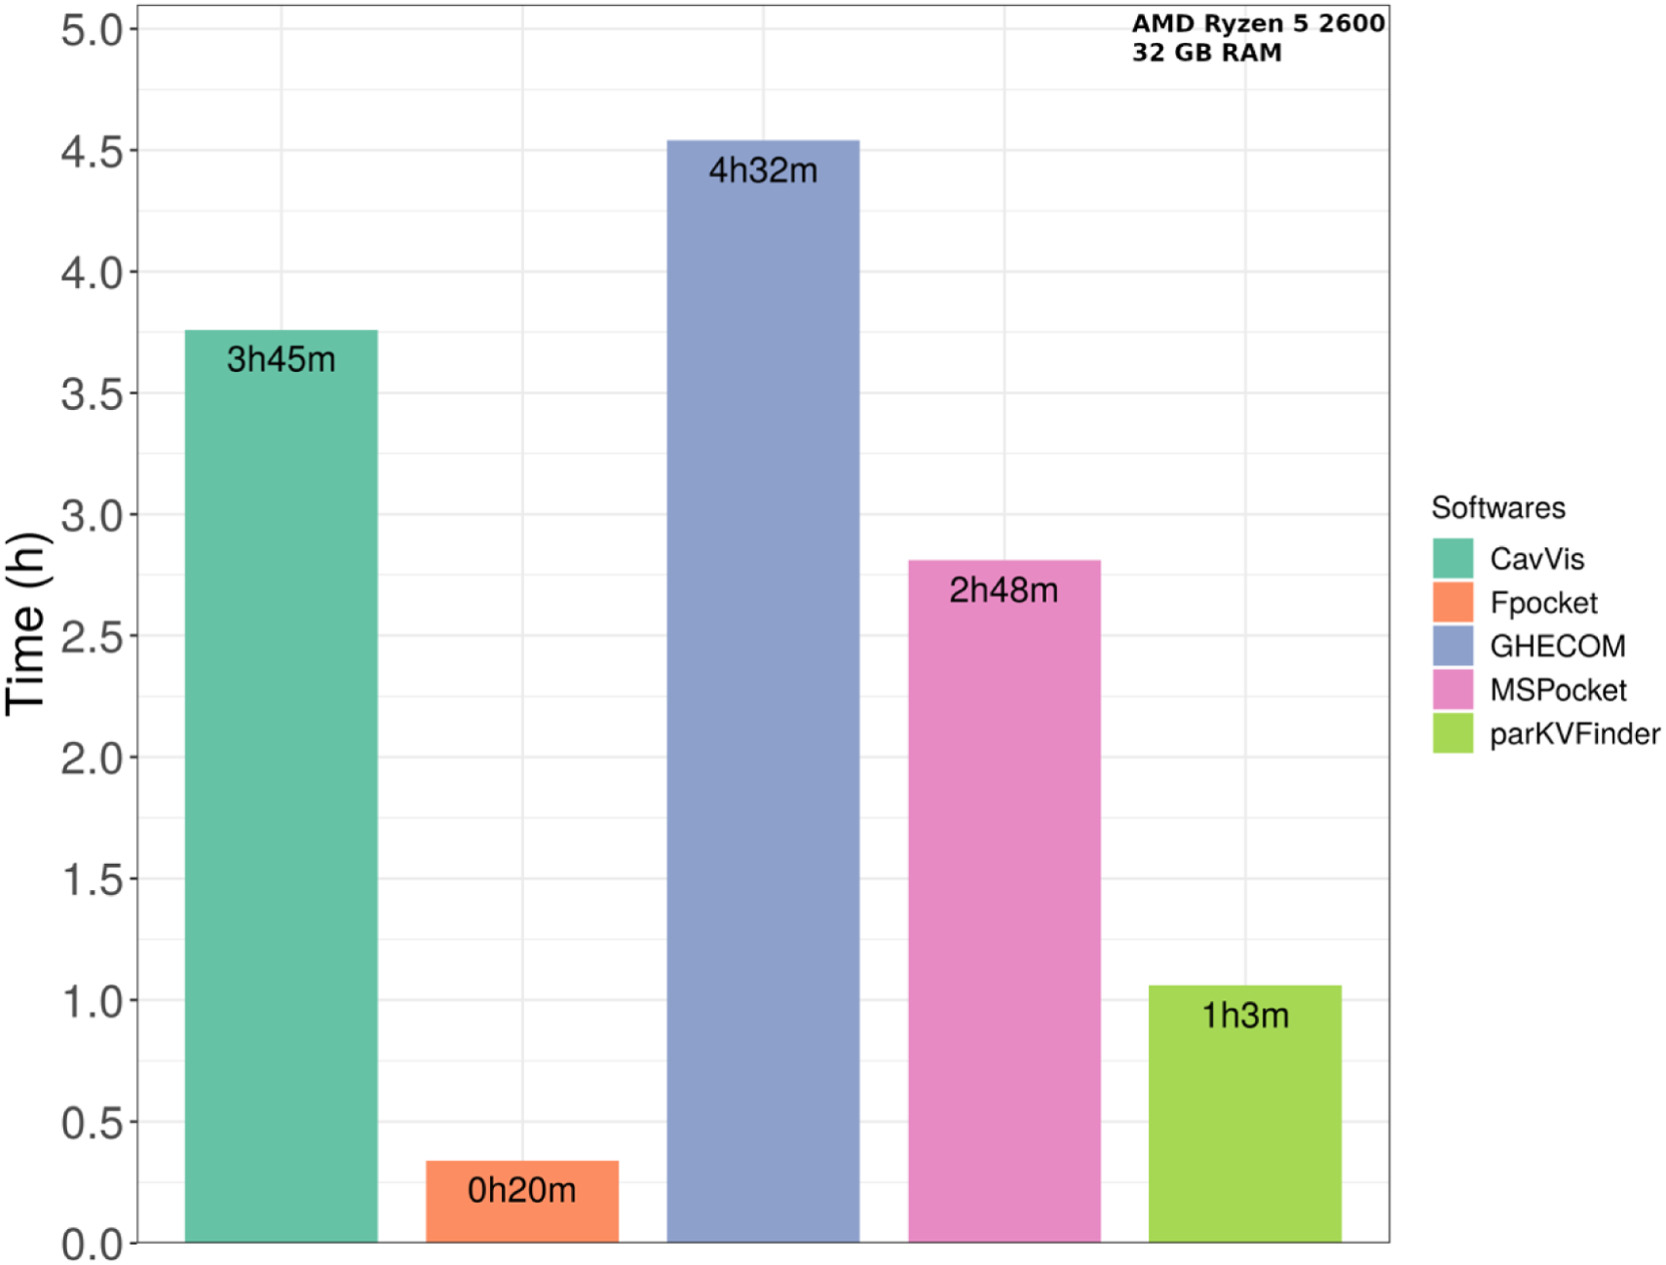
\includegraphics[scale=0.9]{images/hiv1-protease-dm-times.png}}
  \centerline{\tiny{\textbf{Source:} Reprinted from \cite{guerra2020}. Licensed under \href{https://creativecommons.org/licenses/by/4.0/}{CC BY 4.0}.}}
  \caption[Computational time of the benchmarking methods]{\textbf{Computational time of the benchmarking methods.}}
  \label{fig:hiv1-protease-dm-times}
\end{figure}

It is important to highlight that the details of the simulations and analyses are available in the article published in the \textit{SoftwareX} journal \cite{guerra2020}.

\subsection{Mayaro and other alphaviruses}

\ac{MAYV} is an emerging arbovirus prevalent in Central and South America, associated with a debilitating and arthritogenic disease. The ectodmains E1 and E2 are essential transmembrane alphaviral proteins that form heterodimers. These heterodimers, organized into trimers, compose the spikes on the viral surface, extending through the lipid bilayer and interacting with the nucleocapsid proteins C. These spikes play a crucial role in binding to cellular receptors, cell internalization, and membrane fusion. The subsquent release of \acs{MAYV} RNA into the cytoplasm triggers viral protein expression, replication, and the production of mature and infectious viral progeny. Given their central role, the E1 and E2 proteins of \acs{MAYV} are key targets for vaccine development and antiviral drugs \cite{ribeiro2021}. However, the lack of detailed structural information on these proteins has hindered the development of effective strategies to combat \acs{MAYV} infection.

The central region between the E1 and E2 proteins forms a cavity occupied by an extra-long density, not accounted for by side-chain residues (Figure \ref{fig:mayv-e1-e2}A and B). A similar density profile was previously observed in a cryo-electron map of the \ac{SINV}, suggesting a hydrophobic phospholipid tail (C18), termed a \textit{pocket factor}, might occupy this density and stabilize the hydrophobic pocket formed between E1 and E2 \cite{chen2018}. To gain a deeper understanding of the pocket environment and extract its chemical characteristics, we employed parKVFinder \cite{guerra2020} to comprehensively characterize the \acs{MAYV} pocket and compare it with pockets in other alphaviruses. The E1 and E2 ectodomains of \acs{MAYV} (PDB ID: 7KO8), \acs{SINV} (PDB ID: 6IMM), \ac{EEEV} (PDB ID: 6MX4), \ac{VEEV} (PDB ID: 3J0C), and \ac{CHIKV} (PDB ID: 6NK5) were used for the detection and characterization of the hydrophobic pocket. In \acs{MAYV}, the cavity between the E1 and E2 domains has a volume of $\sim$850 $\AA^3$ (Figure \ref{fig:mayv-e1-e2}D). This volume is quite similar across \acs{SINV}, \acs{EEEV}, and \acs{VEEV}, while in \acs{CHIKV}, the larger distance between E1 and E2 results in a larger volume.

\begin{figure}
  \centerline{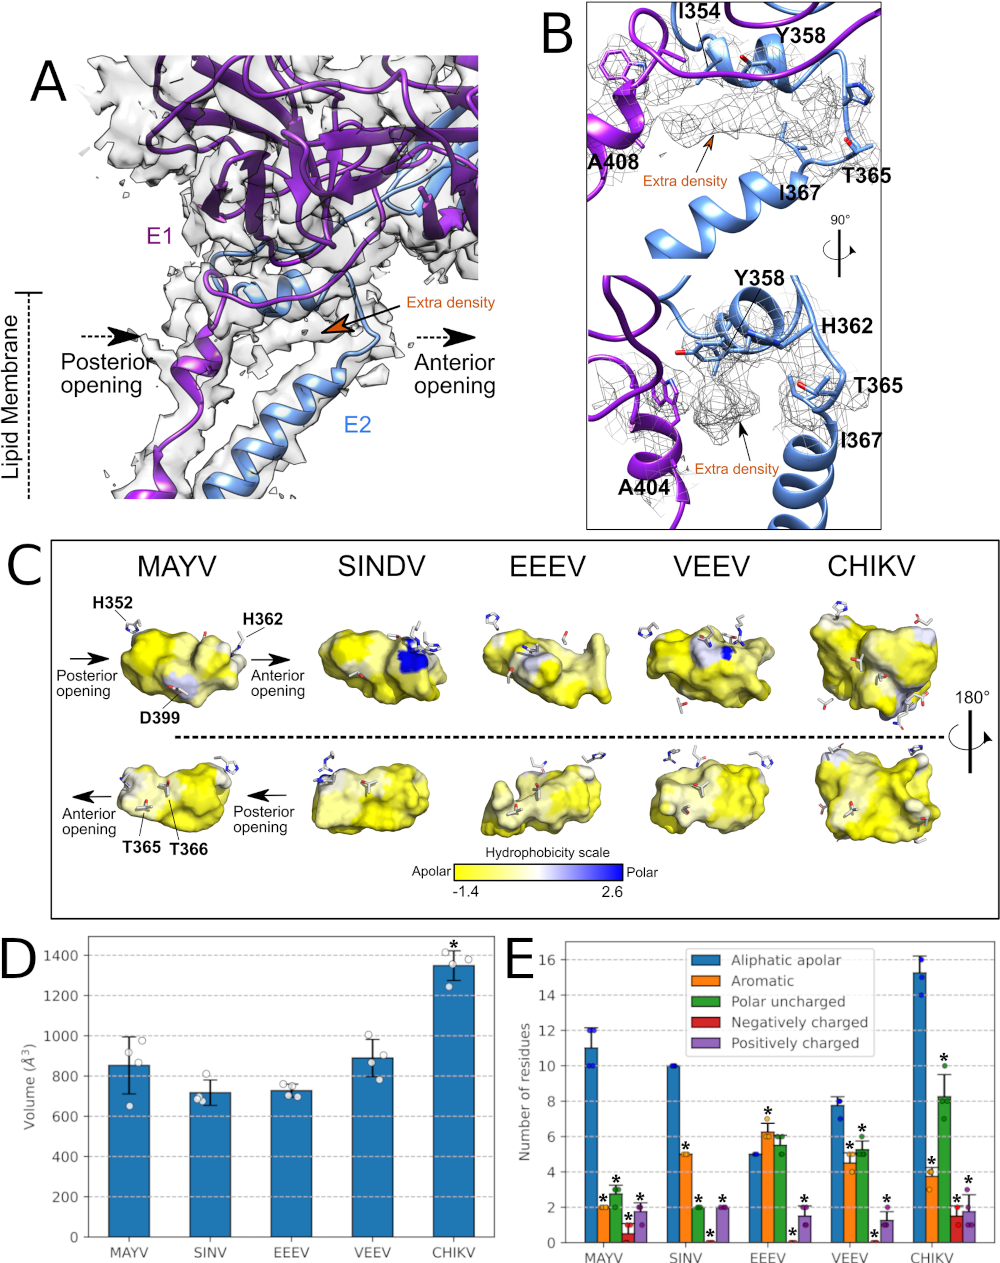
\includegraphics[scale=0.22]{images/mayv-e1-e2.png}}
  \centerline{\tiny{\textbf{Source:} Adapted from \cite{ribeiro2021}. Licensed under \href{https://creativecommons.org/licenses/by/4.0/}{CC BY 4.0}.}}
  \caption[MAYV E1 and E2 transmembrane domains and the hydrophobic cavity]{\textbf{MAYV E1 and E2 transmembrane domains and the hydrophobic cavity.} \textbf{(A)} \acs{3D} atomic model of \acs{MAYV} fitted to the density map, showing the upper portion of the E1 and E2 TM helices. The E1-E2 intersection forms a cavity with anterior and posterior openings. The observed extra density within the cavity is indicated. \textbf{(B)} Detail of the extra density found in the head region of E1-E2 and the surrounding residues. The density map of \acs{MAYV} is shown in mesh or surface representation. \textbf{(C)} Cavity detection in alphaviral structures. The cavity between the E1 and E2 domains is shown in surface representation and colored based on the Eisenberg & Weiss hydrophobicity scale, using the residues that form the cavity. Only polar residues are represented as sticks. \textbf{(D)} Cavity volume for the four E1-E2 heterodimers (n = 4 independent heterodimer structures) in the asymmetric unit. One-way ANOVA with Tukey's multiple comparison test was used to compare the \acs{MAYV} cavity volume with other alphaviruses (* indicates adj. p < 0.01 when compared to alphaviruses with \acs{MAYV}). \textbf{(E)} Number of residues in each of the four E1-E2 heterodimers (n = 4 independent heterodimer structures) in the asymmetric unit, separated by classes. One-way ANOVA with Tukey's multiple comparison test was used to compare the number of residues in the apolar aliphatic class with the other classes in the same alphavirus species (* indicates adj. p < 0.01 when comparing the apolar aliphatic class with the other classes). All data are presented as mean values +/- SD. Apolar aliphatic: ALA, VAL, ILE, LEU, GLY, PRO; Aromatic: PHE, TYR, TRP; Uncharged polar: SER, THR, CYS, MET, ASN, GLN; Negatively charged: GLU, ASP; Positively charged: ARG, LYS, HIS.}
  \label{fig:mayv-e1-e2}
\end{figure}

The hydrophobic nature of the alphavirus pocket is clearly observed by mapping the hydrophobicity surface (Figure \ref{fig:mayv-e1-e2}C) and the number of apolar residues forming the core of the cavity (Figure \ref{fig:mayv-e1-e2}E). The pocket density extends to polar residues, such as H362, T365, and T366 from the E2 domain at the posterior opening (Figure \ref{fig:mayv-e1-e2}C and E), indicating that the molecule may have an amphipathic nature, such as a fatty acid. Notably, T365 and T366 maintain a structurally conserved position in other alphaviruses or are replaced by serine, an even more polar residue. At the posterior opening, another histidine (H352 from E2) helps close the pocket, with histidine residues in similar positions observed in most alphaviruses, except SINV. Together, these findings indicate that alphaviruses have a consistent amphipathic cavity formed between the E1 and E2 domains in the outer membrane of the lipid bilayer. If the alphaviral pocket hosts a molecule, it would be chemically similar across different alphaviruses. The density map of \acs{MAYV} suggests that the extra density may be occupied by a fatty acid, potentially enhancing interactions between E1 and E2. Consequently, the pocket emerges as a potential target for the development of antiviral compounds against \acs{MAYV} and other alphaviruses through rational drug design.

On the other hand, alphavirus nucleocapsid proteins C are composed of two subdomains: a disordered N-terminal domain, responsible for binding to viral RNA (not observed in the \acs{MAYV} density map), and a structured C-terminal domain that non-covalently binds to E2 proteins (Figure \ref{fig:mayv-c-e2}). The N-terminal region has lower identity among alphaviruses and is reported as virus-specific \cite{ribeiro2021}. The \acs{MAYV} density map confirms the generally conserved structure of the C protein, forming two subdomains rich in beta sheets separated by a shallow cavity of $\sim$500 $\AA^3$ (Figure \ref{fig:mayv-c-e2}), wherein the C-terminal domain of the E2 protein non-covalently binds. The bottom of the pocket is hydrophobic, while its top has polar and charged residues. The interface between the capsid and the E2 protein involves the TPY consensus motif (residues T387, P398, and Y399; Figure \ref{fig:mayv-c-e2}), conserved within the \textit{Alphavirus} genus. Interestingly, small molecules proposed to inhibit the interaction between the capsid and the E2 protein contain heterocyclic rings, reinforcing the relevance of this type of contact for the capsid-E2 protein interaction and positioning this site as a potential drug target.

\begin{figure}[hp]
  \centerline{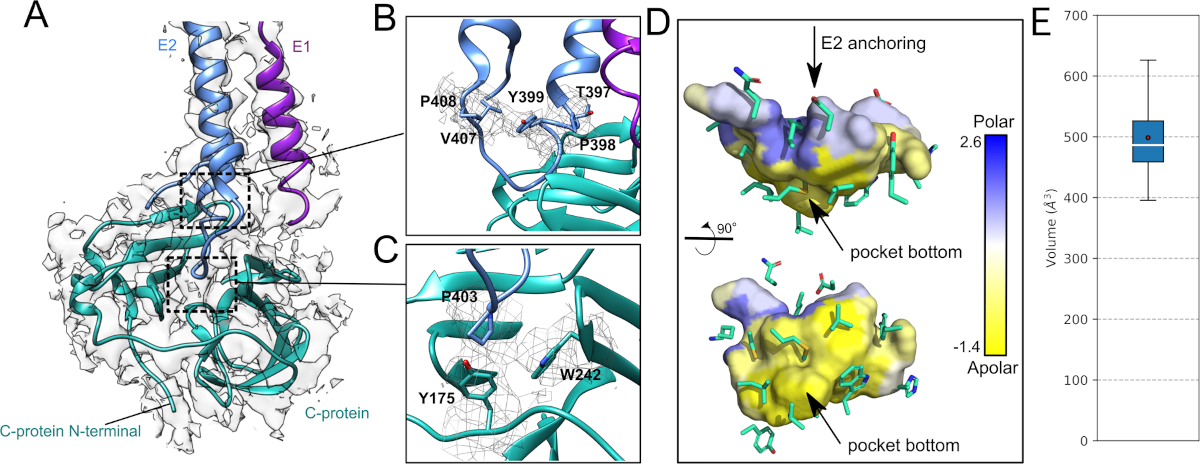
\includegraphics[scale=1]{images/mayv-c-e2.png}}
  \centerline{\tiny{\textbf{Source:} Adapted from \cite{ribeiro2021}. Licensed under \href{https://creativecommons.org/licenses/by/4.0/}{CC BY 4.0}.}}
  \caption[Interaction of MAYV capsid with the C-terminal domain of the E2 protein]{\textbf{Interaction of MAYV capsid with the C-terminal domain of the E2 protein.} \textbf{(A)} 3D atomic model of \acs{MAYV} fitted to the density map obtained by cryo-electron microscopy. The C, E1, and E2 proteins are represented as cyan, purple, and blue cartoons, respectively. \textbf{(B)} The interaction of the TPY motif (residues T387, P398, and Y399) with the C protein. \textbf{(C)} Residues P403 and T402 of E2 and their interaction with the aromatic residues Y175 and W242 in the C protein. The density map of \acs{MAYV} is shown in mesh representation. \textbf{(D)} Cavity detection in the C protein of \acs{MAYV}, showing a hydrophobic environment at the bottom of the pocket and a polar and charged environment at the outer edges of the cavity. The cavity in the C protein that binds to the C-terminal domain of E2 is shown in surface representation and colored according to the Eisenberg hydrophobic consensus scale. The C protein residues surrounding the cavity are represented as sticks. \textbf{(E)} Boxplot of the cavity volume for the four capsids (n = 4 independent capsid structures) in the asymmetric unit. In the boxplot, the box represents the interquartile range ($IQR$) ($67.5 \AA^3$), the 75th percentile ($Q3$) ($526.2 \AA^3$), and the 25th percentile ($Q1$) ($458.7 \AA^3$). The central line indicates the median ($486.3 \AA^3$), and the mean ($498.6 \AA^3$) is indicated by a dot. The "whiskers" with a minimum value ($395.7 \AA^3$) and a maximum value ($626.2 \AA^3$) are determined using $Q1-1.5 \cdot IQR$ and $Q3+1.5 \cdot IQR$, respectively.}
  \label{fig:mayv-c-e2}
\end{figure}

It is important to note that the complete results and details of the analyses are available in the article published in the \textit{Nature Communications} journal \cite{ribeiro2021}.

\subsection{Discussion}

parKVFinder emerges as a powerful tool for detecting and characterizing biomolecular cavities, offering enhanced capabilities through integration with PyMOL—a user-friendly platform for visualization. The routine optimization and parallelization have significantly improved its performance, surpassing its predecessor, KVFinder \cite{guerra2019,guerra2020}. In the case study involving the \acs{MD} of HIV-1 protease, parKVFinder demonstrated a remarkable capacity to accurately describe the conformational dynamics of the active site, outperforming other geometry-based methods both in accuracy and computational time. The investigation of the hydrophobic pocket within alphaviruses, particularly in MAYV, not only identifies on potential drug targets but also highlights shared structural features across alphaviruses. This consistency in the nature of the cavity underscores parKVFinder's utility in uncovering fundamental aspects of biomolecular structures.

Despite the successful application of parKVFinder in \acs{MD} simulations \cite{guerra2020} and a comparative study \cite{ribeiro2021}, certain limitations became apparent in automated tasks and systematic binding site comparisons. Consequently, there arises a need for a more suitable tool tailored to data science applications, providing straightforward access to functions and data structures for efficient analysis. Nevertheless, it is important to acknowledge that parKVFinder still plays a significant role within KVFinder suite. Its contribution lies notably in optimizing detection and characterization parameters through the PyMOL graphical plugin (PyMOL2 parKVFinder Tools), leveraging its visual cues. These fine-tuned parameters seamlessly integrate into automated studies and systematic binding site comparisons. In essence, parKVFinder continues to be indispensable for conducting structural and functional analyses focused on individual biomolecular structures.

\section{pyKVFinder}

In data science, data-intensive cavity analysis demand efficient routines and algorithms built on easily manipulable data structures. Cavities identified by parKVFinder, like those in other well-known programs such as fpocket \cite{fpocket}, GHECOM \cite{ghecom}, and POVME 3.0 \cite{povme}, are human-readable and easily displayed in molecular visualization programs. However, they lack suitable structuring for direct integration into automated protocols or data science applications. Addressing this need, we developed the \ac{pyKVFinder} \cite{guerra2021}, an open-source Python package, licensed under GPL v3.0, for cavity detection and characterization in biomolecular structures within automated protocols and data science applications. Subsequently, pyKVFinder was published in BMC Bioinformatics \cite{guerra2021} and released as pyKVFinder \href{https://github.com/LBC-LNBio/pyKVFinder/tree/v0.2.5}{pyKVFinder v0.2.5}, with the current version being \href{https://github.com/LBC-LNBio/pyKVFinder/tree/v0.6.9}{v0.6.9}. The source code is under continuous development and available at the following repository: https://github.com/LBC-LNBio/pyKVFinder.

pyKVFinder employs a \ac{SWIG} (\url{https://www.swig.org}) to extend \acs{3D} grid operations, written in C, to the high-level programming language, Python. In pyKVFinder, the target biomolecule is inserted in a regular 3D grid, stored as an \ac{ndarray} from the NumPy package \cite{numpy}. To detect cavities, the tool uses a dual-probe algorithm, as shown in Figure \ref{fig:parkvfinder-schema}, which scans the biomolecular structure for regions of inaccessibility (\ie, cavities). In addition to cavity properties like volume, area, and interface residues stored as Python dictionaries, pyKVFinder calculates cavity depth and hydrophobicity. Both cavity points and these morphological and physicochemical properties are stored in \acsp{ndarray} and can be visualized using Python molecular visualization packages (\eg, NGLView \cite{nglview} and plotly \cite{plotly}). Moreover, pyKVFinder can be integrated with various scientific packages and libraries (\eg, scikit-learn \cite{scikit-learn} and SciPy \cite{scipy}) for mathematical calculations, statistical analysis, and \acs{3D} visualization using interactive interfaces (\eg, IPython, Jupyter, and JupyterLab notebooks). Thus, pyKVFinder facilitates complex analyses of biostructural data with protocols and algorithms within the Python ecosystem, serving as a building block for new applications in data science, rational drug design, and drug discovery. In essence, pyKVFinder provides a versatile means of detecting and characterizing biomolecular cavities and integrating this information into automated protocols and data science applications.

\begin{figure}[ht]
  \centering
  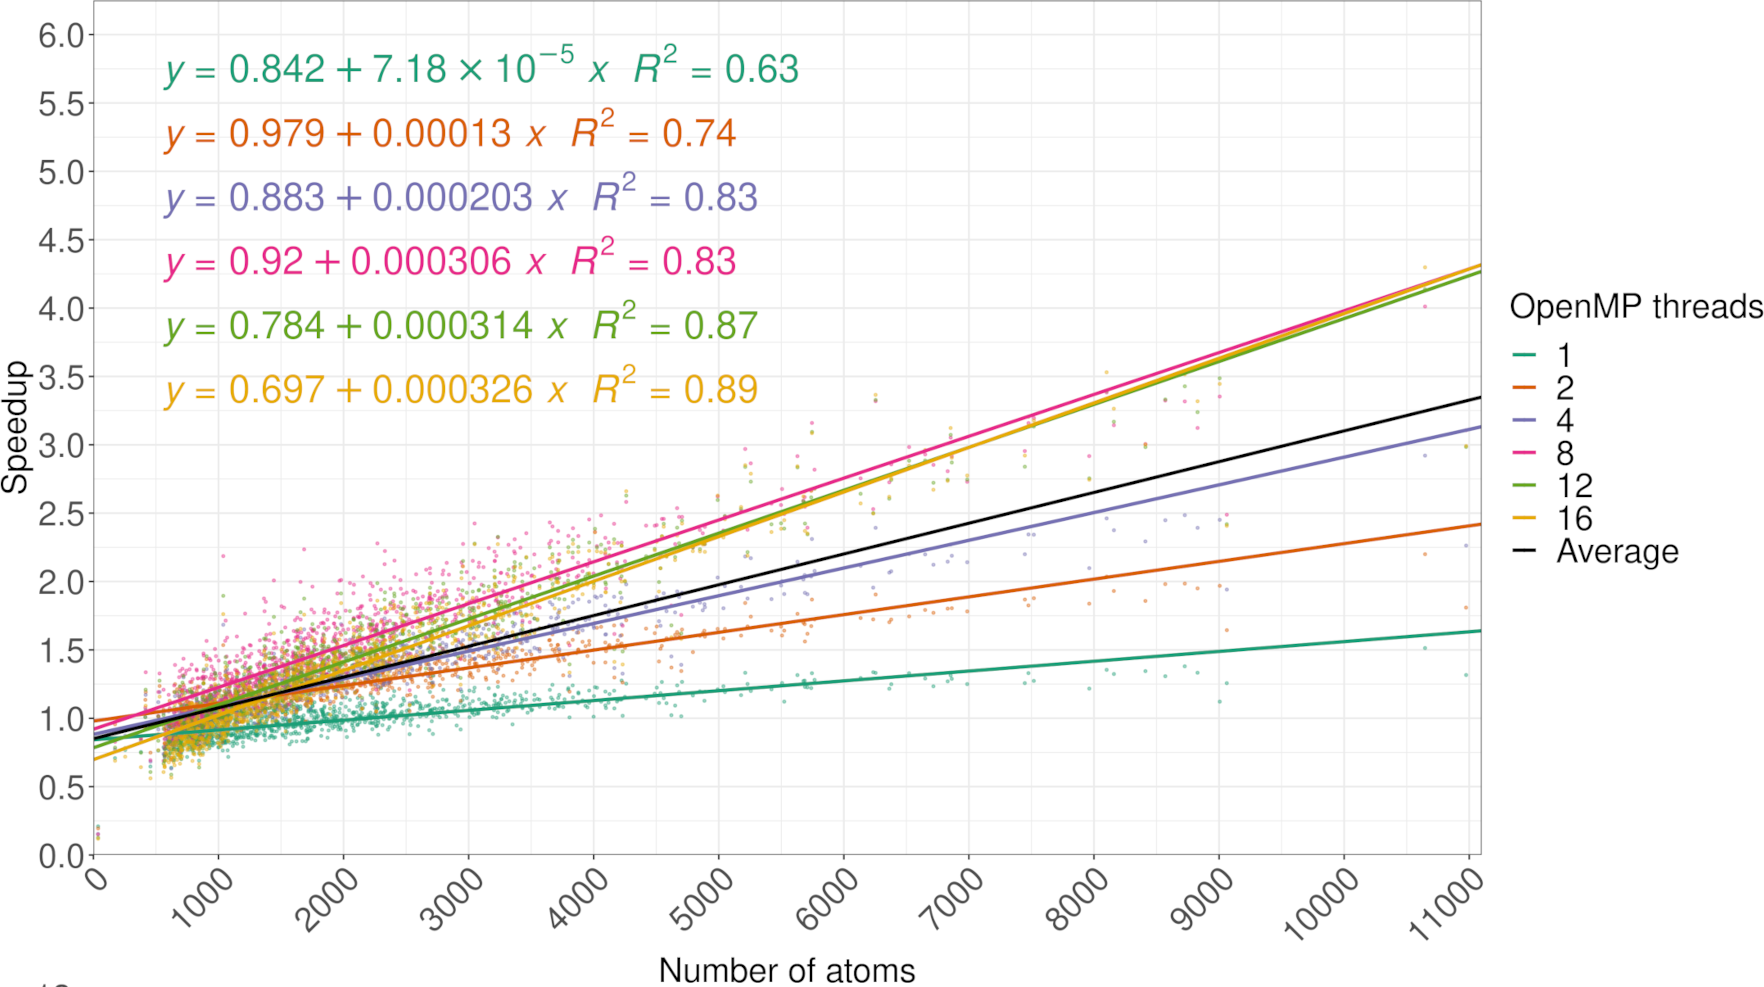
\includegraphics[scale=1]{images/pykvfinder-speedup.png}
  \caption[Speedup of pyKVFinder compared to parKVFinder]{\textbf{Speedup of pyKVFinder compared to parKVFinder.} The speedup is the ratio of pyKVFinder's execution time to parKVFinder's execution time, applying the same number of OpenMP threads, for different numbers of atoms.}
  \label{fig:pykvfinder-speedup}
\end{figure}

The computational performance of pyKVFinder was also assessed on kv1000 \cite{guerra2020}, exhibiting a considerably shorter runtime compared to parKVFinder, averaging 31\% faster (Figure \ref{fig:pykvfinder-speedup}). Even with the addition of new characterizations such as depth and hydrophobicity, pyKVFinder's performance was only reduced by an average of 5\% (for depth) and 4\% (for hydrophobicity), regardless of the number of threads used (Figure \ref{fig:pykvfinder-parkvfinder-kv1000-comparison}). The primary reason for this performance gain lies in the additional possibility to parallelize routines, \ie, atom insertion into the 3D grid in the detection function (\ie, \textit{pyKVFinder.detect}), based on \acsp{ndarray}. The most significant improvement was observed in proteins with over 2000 atoms, achieving a speedup of $\sim$4.3 times in proteins with 11000 atoms, benefiting the growing number of currently resolved high-order structures. For very small proteins ($\less 2000$ atoms), which represent a smaller portion of available structures, pyKVFinder's performance gain was not significant or even lower than that of parKVFinder, mainly due to the Python reading of the target's PDB or XYZ file (Figure \ref{fig:pykvfinder-speedup}). Therefore, experienced users requiring scripting routines are encouraged to use pyKVFinder due to its enhanced performance, while beginners should prioritize parKVFinder due to its monolithic behavior and ease of installation and execution. Additionally, the scalability of pyKVFinder with an increasing number of threads, as well as the absolute time to perform cavity detection, is presented in Figure \ref{fig:pykvfinder-parkvfinder-kv1000-comparison}, following the behavior exhibited by parKVFinder \cite{guerra2020}.

\begin{figure}[h]
  \centering
  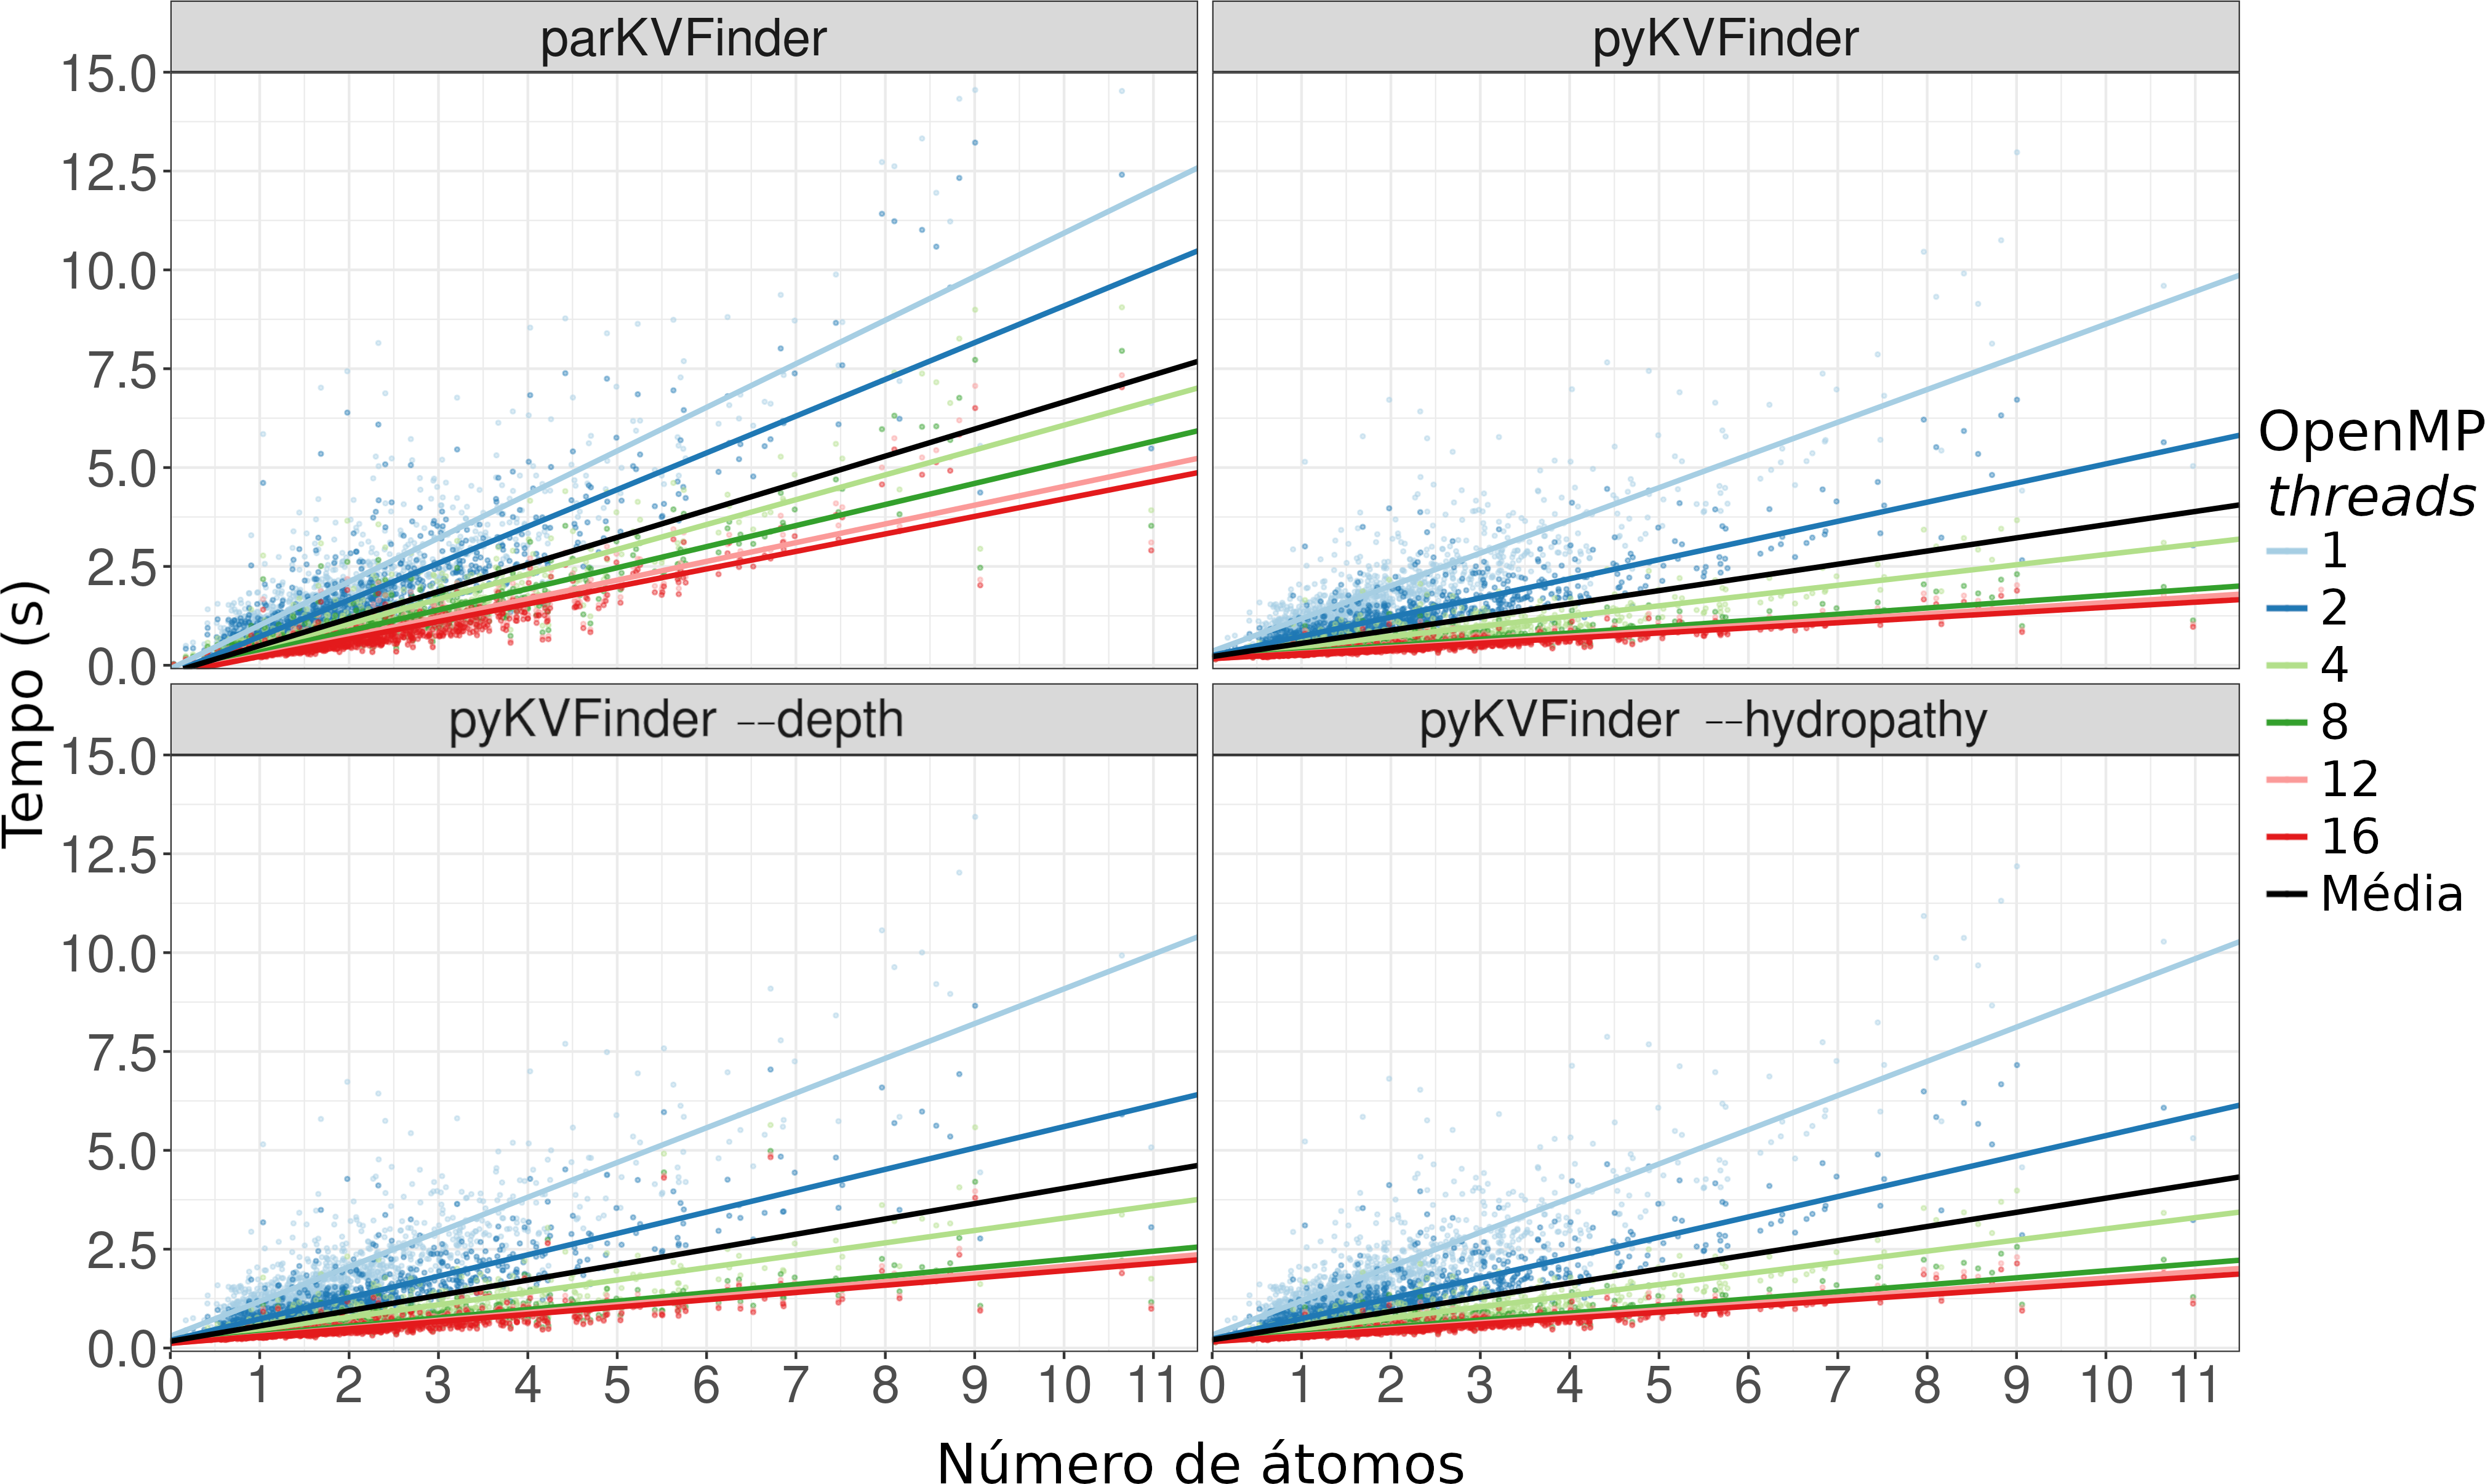
\includegraphics[scale=0.95]{images/pykvfinder-parkvfinder-kv1000-comparison.png}
  \caption[Computational time as a function of the number of atoms with different numbers of threads for parKVFinder and pyKVFinder]{\textbf{Computational time as a function of the number of atoms with different numbers of threads for parKVFinder and pyKVFinder.} Top left panel: parKVFinder. Top right panel: pyKVFinder with default characterization (volume, area, and interface residues). Bottom left panel: pyKVFinder with default and depth characterizations. Bottom right panel: pyKVFinder with default and hydrophobicity characterizations.}
  \label{fig:pykvfinder-parkvfinder-kv1000-comparison}
\end{figure}

% \subsection{Implementações de novas caracterizações}

% Dentro do contexto do pyKVFinder, em colaboração com o Dr. György Szalóki (Laboratoire Hétérochimie Fondamentale et Appliquée - Université Toulouse III Paul Sabatier - França), o escopo do KVFinder suite foi expandido para uma nova classe de moléculas chamadas de gaiolas supramoleculares. Essas gaiolas são moléculas interconectadas que se unem de forma não-covalente, formando uma cavidade interna capaz de encapsular moléculas ou íons. A forma e o tamanho da cavidade são parâmetros importantes que podem ser facilmente determinados por algoritmos geométricos, auxiliando no desenho racional de gaiolas supramoleculares. Nesse contexto, também foram desenvolvidas novas caracterizações aplicáveis tanto para o contexto de gaiolas quanto para biomoléculas.

% \subsubsection{Estimativa do volume molecular}

% Para a modelagem da superfície molecular, desenvolvemos a classe \textit{Molecule} no pyKVFinder, que permite a modelagem das superfícies moleculares, conforme ilustrado na Figura \ref{fig:surface-representation}, e estimativa do volume molecular, como apresentado na Figura \ref{fig:molecular-modeling}. Nessa abordagem, as moléculas são inseridas em uma grade 3D regular, levando em consideração os raios de vdW de cada um dos átomos da molécula. Os usuários tem a flexibilidade de definir esses raios por meio de um arquivo de configuração (\textit{\href{https://github.com/LBC-LNBio/pyKVFinder/blob/master/pyKVFinder/data/vdw.dat}{vdw.dat}}), assim como a representação de superfície escolhida. Na grade 3D, cada voxel corresponde a um ponto de molécula (0) ou de solvente (1). Portanto, o volume de van der Waals da molécula é estimado somando-se os voxels rotulados como molécula na grade 3D. Essa funcionalidade de estimativa do volume molecular está disponível no pyKVFinder a partir da versão \href{https://github.com/LBC-LNBio/pyKVFinder/tree/v0.5.0}{v0.5.0}. A implementação desses recursos de modelagem e caracterização de moléculas foi detalhada e aplicadas em um artigo publicado no periódico \textit{Journal of Chemical Information and Modeling} \cite{guerra2023B}.

% \begin{figure}[ht]
%   \centering
%   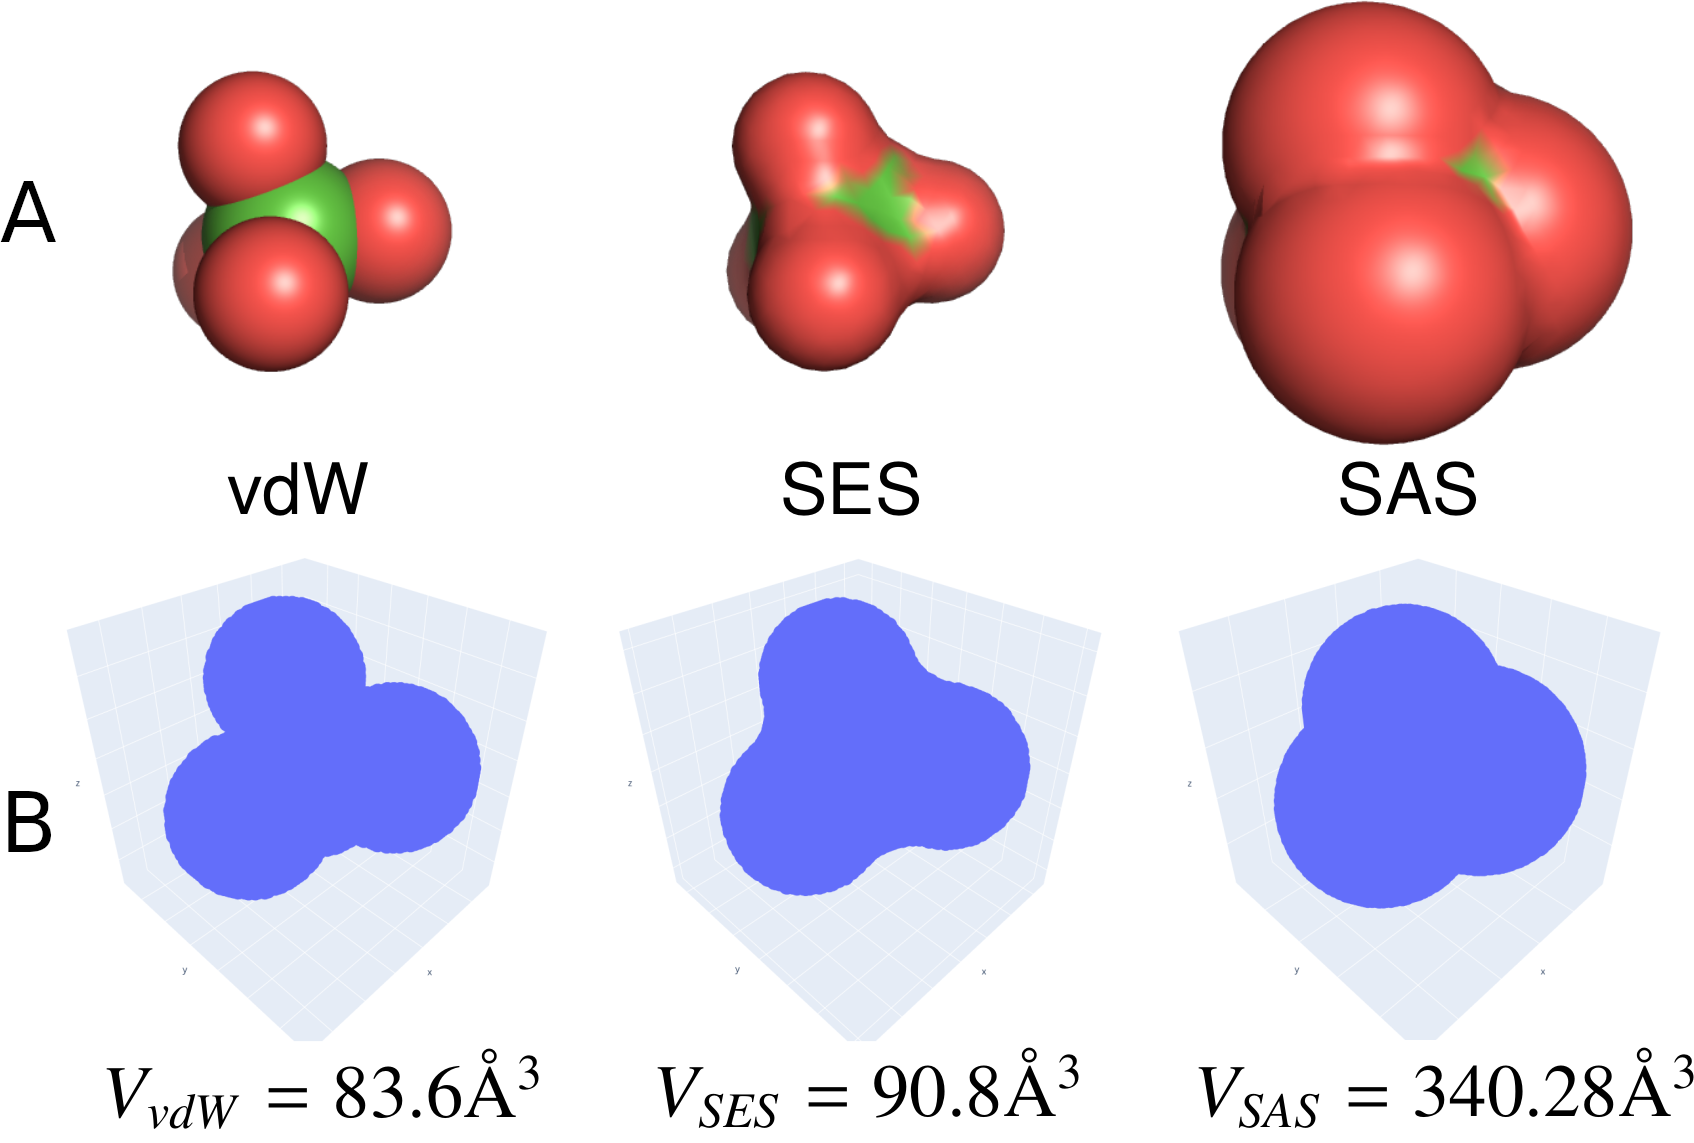
\includegraphics[scale=1.5]{images/molecular-modeling.png}
%   \caption[Modelagem e estimativa de volume molecular do perclorato ($ClO_4$)]{\textbf{Modelagem e estimativa de volume molecular do perclorato ($ClO_4$).} \textbf{(A)} Superfície molecular de vdW (quadro esquerdo), SES (quadro central) e SAS (quadro direito) no visualizador molecular PyMOL. \textbf{(B)} Modelagem e estimativa do volume molecular de vdW (quadro esquerdo), SES (quadro central) e SAS (quadro direito) pelo pyKVFinder.}
%   \label{fig:molecular-modeling}
% \end{figure}

% \subsubsection{Caracterização de aberturas}

% A compreensão das características das gaiolas supramoleculares, como volume (Figura \ref{fig:cage-characterization}A) e abertura (Figura \ref{fig:cage-characterization}B), que impulsionam o encapsulamento de intermediários reativos é fundamental para o desenho racional de novas gaiolas supramoleculares com propriedades catalíticas aprimoradas. Nesse sentido, desenvolvemos uma caracterização de abertura utilizando o pyKVFinder, que permite a identificação das aberturas, a determinação da área dessas aberturas e a maior sonda esférica (\ie, átomo) que pode passar por cada abertura, conforme ilustrado na Figura \ref{fig:cage-characterization}. 

% \begin{figure}[htb]
%   \centering
%   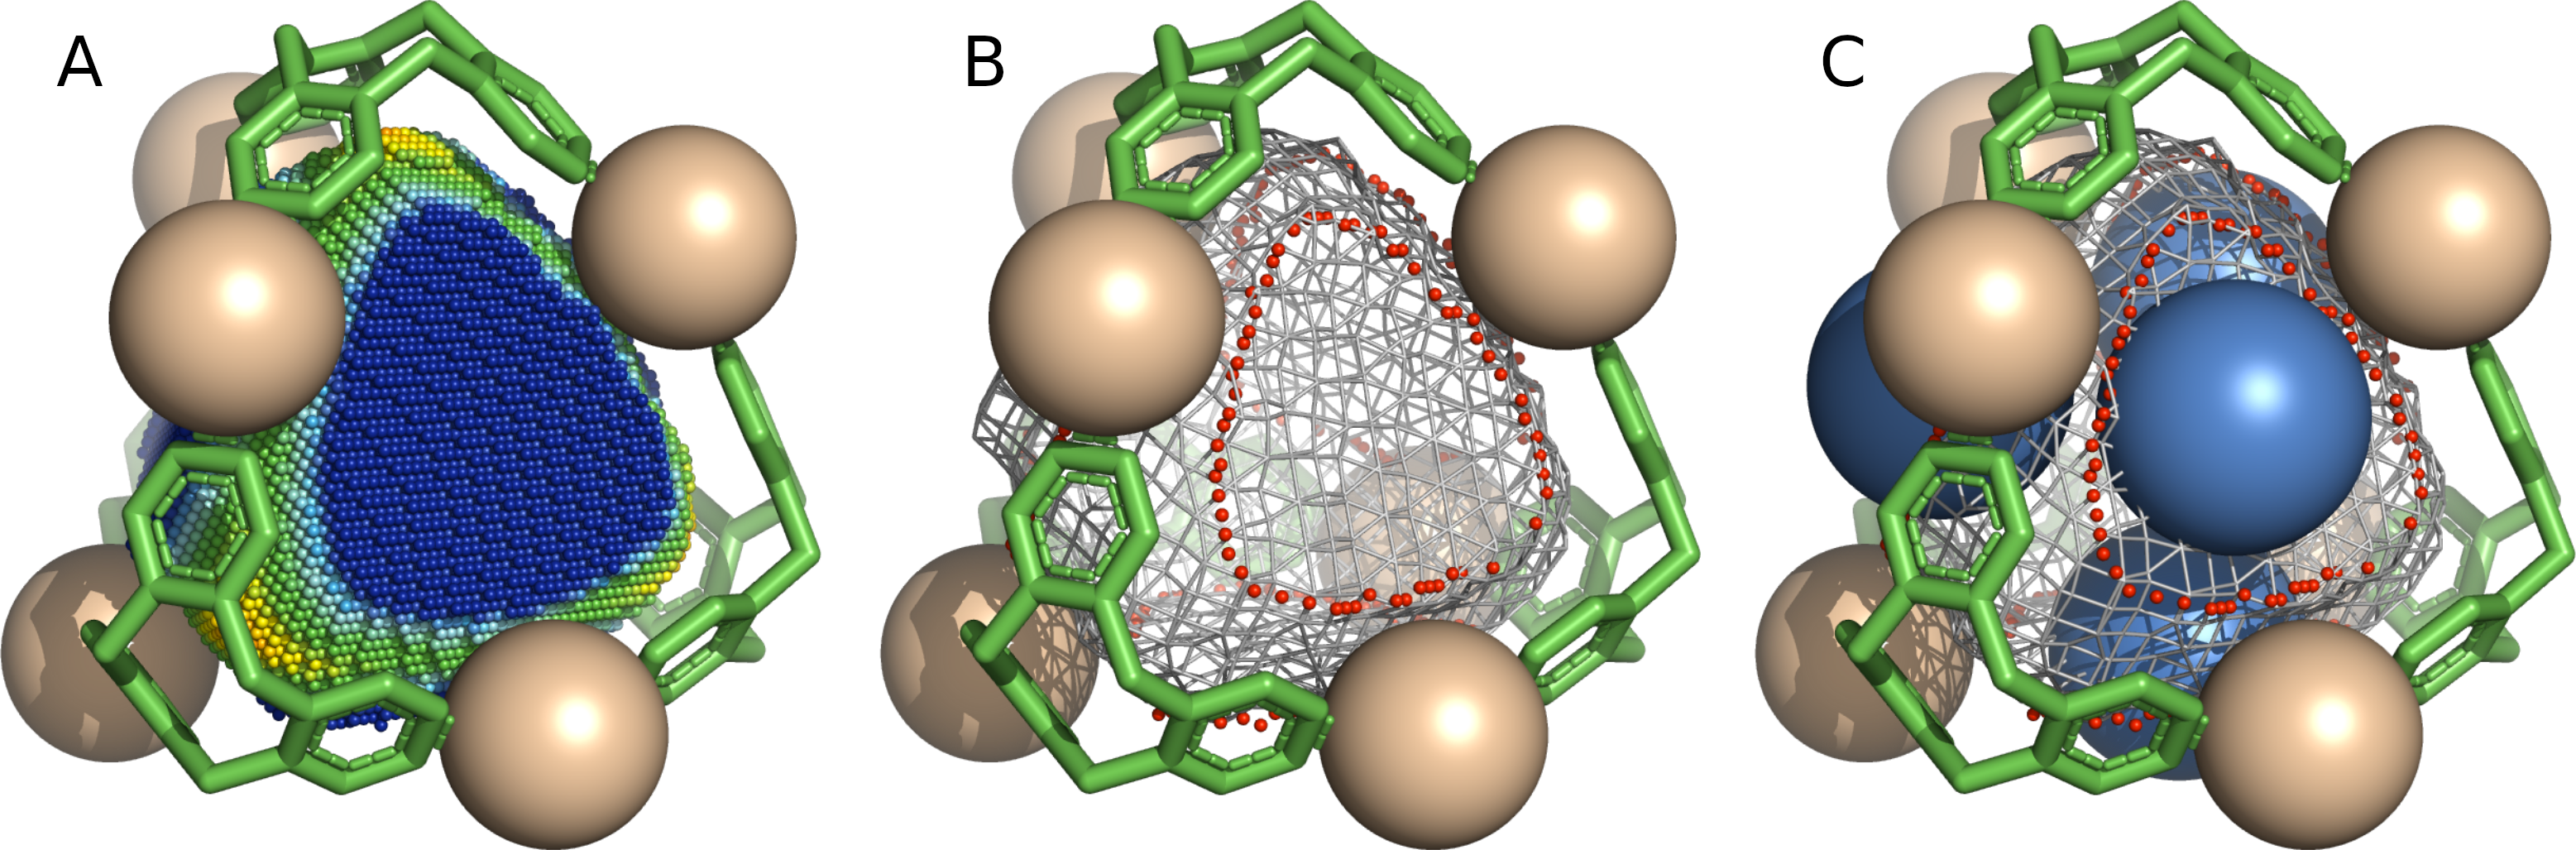
\includegraphics[scale=1.1]{images/cage-characterization.png}
%   \caption[Caracterizações de gaiolas supramoleculares]{\textbf{Caracterizações de gaiolas supramoleculares.} \textbf{(A)} Volume e profundidade. Os pontos são coloridos de acordo a profundidade, sendo azul para menor profundidade e vermelho para maior profundidade. \textbf{(B)} Abertura (pontos vermelhos) e área da abertura. \textbf{(C)} Maior sonda esférica (esfera azul) acessível à cavidade da gaiola.}
%   \label{fig:cage-characterization}
% \end{figure}

% O sistema de dupla sonda utiliza identificadores inteiros para os pontos de cavidade (1), pontos de biomolécula (0) e pontos de meio (-1). Após a agrupamento dos pontos de cavidade pelo algoritmo \textit{Depth-First Search} (DFS), os pontos de cavidade são marcados com valores >2, e os pontos de cavidades que não atingiram o volume de corte (parâmetro \textit{volume cutoff}) são mantidos com o valor 1. Nessa abordagem, os pontos de cavidade localizados a uma unidade de grade de um ponto de meio, seguindo a relação do elemento estruturante de \textit{rank} 3 e conectividade 1 (Figura \ref{fig:elementos-estruturantes}), são identificados como pontos de fronteira cavidade-meio, que são marcados com o valor negativo do identificador numérico da cavidade correspondente, conforme descrito para o cálculo de profundidade \cite{guerra2019,guerra2021}. A partir desses pontos de fronteira, é calculada a área superficial utilizando o procedimento de estimativa de área da plataforma KVFinder suite \cite{guerra2019,guerra2020}, que é equivalente à área da abertura. Em seguida, os pontos de fronteira cavidade-meio localizados a uma unidade de grade de um ponto de biomolécula, seguindo a relação do elemento estruturante de \textit{rank} 3 e conectividade 1 (Figura \ref{fig:elementos-estruturantes}), são identificados como pontos de abertura. Nesse estágio, uma nova grade 3D é gerada para acumular os pontos de abertura, que são marcados com o valor 1, enquanto os demais pontos recebem o valor 0. Após o agrupamento dos pontos de abertura pelo algoritmo DFS, os pontos de abertura são marcados com valores >2 (Figura \ref{fig:cage-characterization}B), e aberturas com menos pontos do que um corte definido pelo usuário são marcadas com o valor 1. Por fim, para cada abertura identificada, é calculado o ponto médio e a maior esfera é determinada a partir desse ponto médio, definindo assim o maior átomo que pode passar por essa abertura (Figura \ref{fig:cage-characterization}C).

% \subsection{Casos de estudo}

% O pyKVFinder foi aplicado em dois casos de estudo publicados em periódicos científicos para investigar proteínas de interesse terapêutico. Essas análises exploraram as características de cavidades de proteínas homólogas ao domínio ADRP do SARS-CoV-2 e a DM do domínio ADRP do SARS-CoV-2 \cite{guerra2021}. No apêndice \ref{ap:casos-de-estudo-pykvfinder}, descreveremos cada um desses casos de estudo em detalhes.

% % A seguir, descreveremos cada um desses casos de estudo em detalhes.

% \subsection{Discussão}

% Apesar de cada método possuir seu próprio conjunto de caracterizações a serem realizadas nas cavidades detectadas, a estrutura de dados das cavidades só é acessível dentro do ecossistema Python no pyKVFinder, que fornece \textit{ndarrays} e dicionários em Python. Ao fornecer uma estrutura de dados acessível e flexível, o pyKVFinder permite aos usuários desenvolver novas caracterizações de cavidades, além de protocolos de análise baseados nessas estruturas de dados. Por exemplo, em um estudo recente conduzido por \cite{jefferson2023}, foi explorada a área transversal das cavidades em proteínas relacionadas usando o pyKVFinder. Esse estudo demonstrou como as estruturas de dados fornecidas pelo pyKVFinder podem ser utilizadas para aprofundar a exploração das cavidades e descobrir informações relevantes para o desenvolvimento de fármacos e a compreensão das interações moleculares. Além disso, a integração do pyKVFinder com o ecossistema Python amplia as possibilidades de análise e visualização de dados, aproveitando as bibliotecas científicas robustas disponíveis nessa linguagem. Essa integração facilita a implementação de análises avançadas e personalizadas, permitindo aos pesquisadores explorar de forma mais abrangente as propriedades das cavidades biomoleculares e obter \textit{insights} valiosos.

% Dessa forma, o pyKVFinder não apenas contribui para o avanço da pesquisa em descoberta e desenho racional de fármacos, mas também fortalece a colaboração e o compartilhamento de conhecimentos na comunidade científica. Ao disponibilizar uma ferramenta acessível, flexível e integrada ao ecossistema Python, o pyKVFinder capacita os pesquisadores a explorar as cavidades biomoleculares de forma mais eficiente e eficaz, impulsionando a descoberta de novos alvos terapêuticos e o desenvolvimento de medicamentos mais eficazes.

\section{KVFinder-web}

% Nos últimos anos, serviços web que se comunicam por meio dos protocolos de transferência de hipertexto (HTTP; \textit{HyperText Transfer Protocol}, em inglês) se tornaram cada vez mais populares em ambientes de computação em nuvem. Esses serviços fornecem amplo acesso a recursos de dados e processamento. Vários serviços web foram propostos para a detecção e/ou caracterização de sítios de ligação em biomoléculas. Entre eles, podemos citar o FpocketWeb \cite{fpocketweb}, GHECOM \cite{ghecom}, CaverWeb \cite{caverweb}, MoloVol \cite{molovol} e 3DLigandSite \cite{3dligandsite}. Em comparação com outras ferramentas para detecção de cavidades, o parKVFinder possui um conjunto intuitivo de parâmetros e foi extensivamente testado na literatura quanto às suas capacidades de detecção e computacionais, oferecendo desempenho preciso e robusto com qualquer tipo de cavidade proteica, conforme ilustrado anteriormente \cite{guerra2019,guerra2020}. Embora outros métodos também possam detectar sítios de ligação proteicos, cada um possui seu conjunto específico de caracterizações. O parKVFinder se destaca por combinar caracterizações morfológicas, topológicas e fisico-químicas de sítios de ligação, auxiliando efetivamente os usuários na identificação de cavidades funcionalmente relevantes e no estudo do processo de reconhecimento molecular.

% \begin{figure}[h]
%   \centering
%   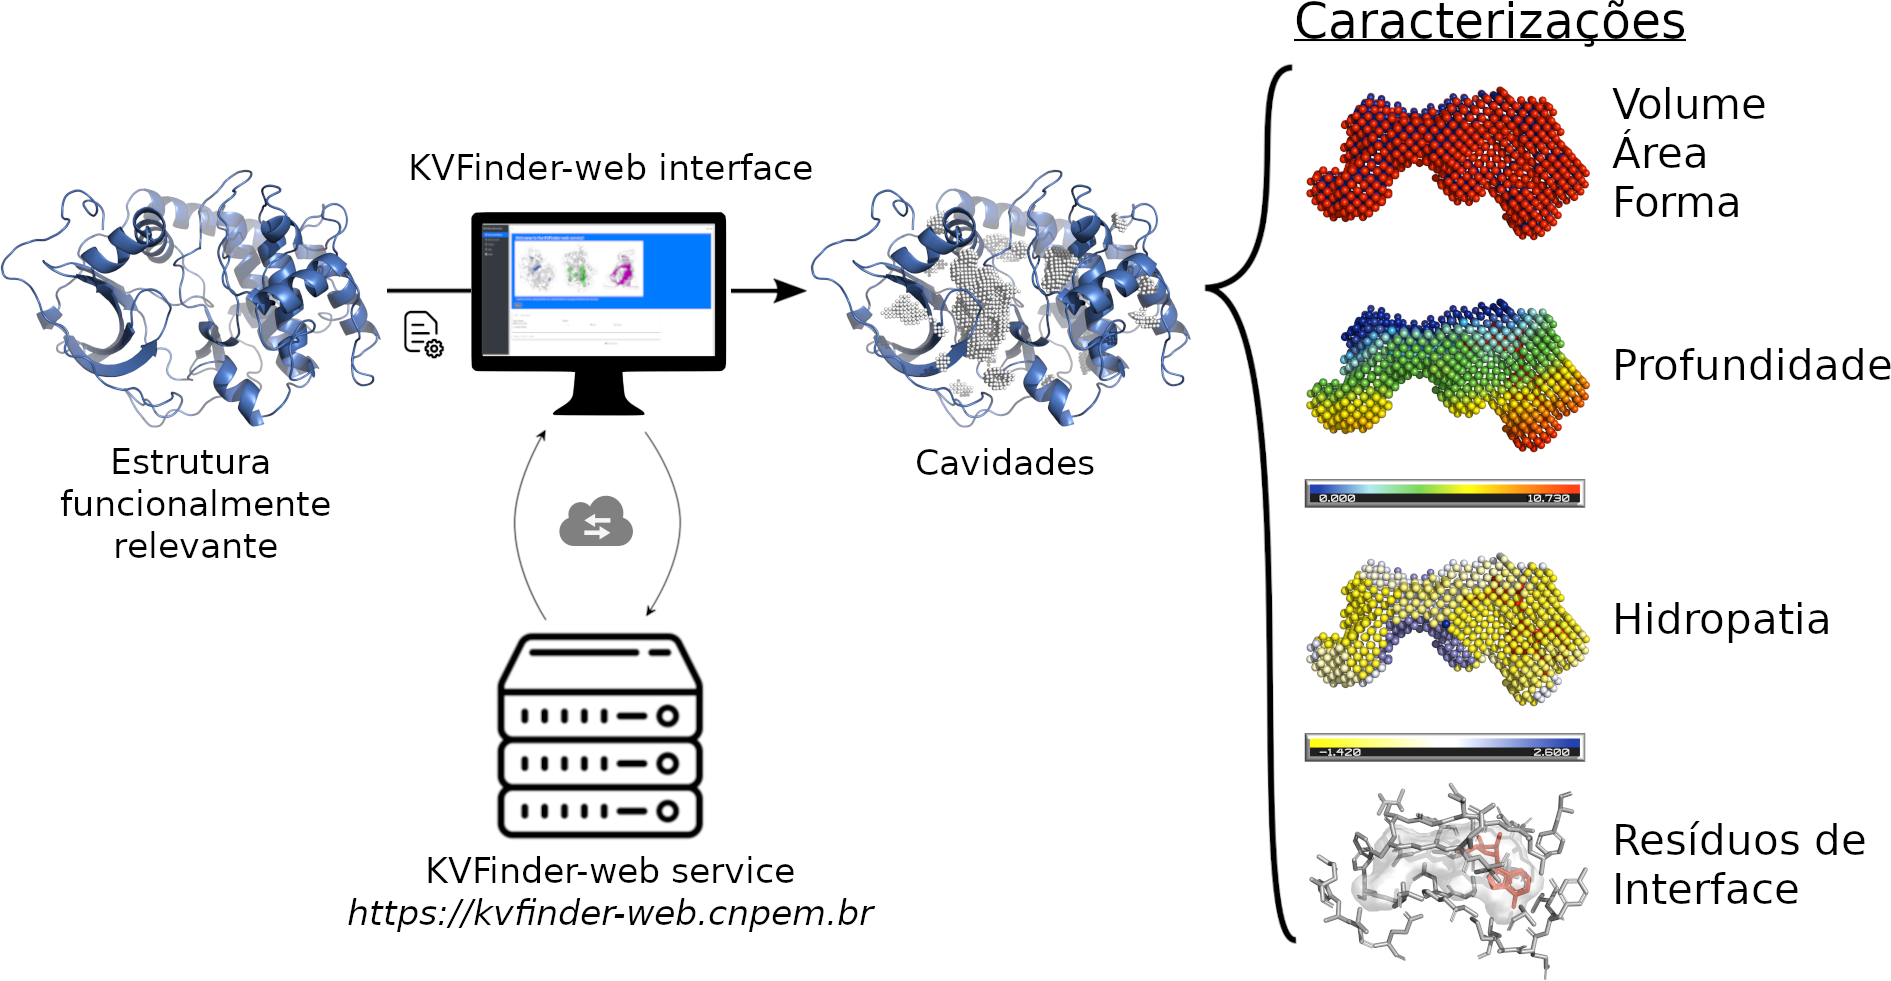
\includegraphics[scale=1.6]{images/kvweb-overview.png}
%   \centerline{\tiny{\textbf{Fonte:} Adaptado de \cite{guerra2023A}.}}
%   \caption[Esquema representativo do funcionamento do KVFinder-web para detectar e caracterizar cavidades em estruturas funcionalmente relevantes]{\textbf{Esquema representativo do funcionamento do KVFinder-web para detectar e caracterizar cavidades em estruturas funcionalmente relevantes.}}
%   \label{fig:kvweb-overview}
% \end{figure}

% Além dos avanços em desempenho e usabilidade do parKVFinder \cite{guerra2019,guerra2020,guerra2023A}, os procedimentos de instalação e configuração da nossa aplicação web, assim como de outras ferramentas independentes para detecção de cavidades, ainda representam uma grande barreira para usuários que não possuem o conhecimento técnico idealmente necessário para executá-los. Além disso, cientistas, educadores e estudantes podem não ter os recursos computacionais locais necessários para os cálculos, o que pode afetar o uso adequado de métodos de detecção e caracterização de cavidades. Nesse cenário, desenvolvemos o \textbf{KVFinder-web}, que foi posteriormente  publicado no periódico \textit{Nucleic Acid Research} \cite{guerra2023A}. O KVFinder-web (Figura \ref{fig:kvweb-overview}), que está disponível em \url{https://kvfinder-web.cnpem.br}, é uma aplicação web de código aberto para detecção e caracterização de cavidades em qualquer tipo de estrutura biomolecular, que consiste em dois componentes independentes: um serviço web RESTful (KVFinder-web service) e uma interface web gráfica (KVFinder-web portal). Para aprimorar ainda mais a experiência do usuário, também fornecemos um plugin gráfico para o PyMOL (PyMOL KVFinder-web Tools).

% \subsection{KVFinder-web portal}

% O \textbf{KVFinder-web portal} (Figura \ref{fig:kvweb-interface}) é uma interface gráfica interativa do KVFinder-web que oferece aos usuários, especialmente os inexperientes, uma aplicação fácil de usar para executar o parKVFinder (v1.2.0) e analisar os resultados por meio de qualquer navegador. Desenvolvido em R Shiny, o KVFinder-web portal fornece um protocolo simples, direto, robusto e interativo para análise e visualização de cavidades, exigindo apenas uma biomolécula no formato PDB ou o código PDB. Atualmente, o KVFinder-web portal está na versão \href{https://github.com/LBC-LNBio/KVFinder-web-portal/tree/v1.1.0}{v1.1.0}. O código-fonte do KVFinder-web portal está disponível no seguinte repositório: \url{https://github.com/LBC-LNBio/KVFinder-web-portal}.

% A interface oferece as principais funcionalidades do KVFinder-web service, permitindo que os usuários carreguem uma biomolécula-alvo a partir de um arquivo PDB ou fornecer o código PDB correspondente, e personalizem os parâmetros de detecção de cavidades e os modos de execução (Figura \ref{fig:kvweb-interface}B). Quatro modos de detecção de cavidades estão disponíveis, oferecendo opções que se adequam melhor à análise da cavidade pelos usuários:

% \begin{itemize}
%   \item \textit{Whole structure (default)}: detecção de cavidades em toda a estrutura biomolecular com parâmetros de detecção pré-definidos;
%   \item \textit{Whole structure (customized)}: detecção de cavidades em toda a estrutura biomolecular com parâmetros de detecção personalizáveis;
%   \item \textit{Around target molecule}: detecção de cavidades dentro de um raio ao redor de cada átomo de um ligante ou molécula na estrutura biomolecular-alvo com parâmetros de detecção personalizáveis;
%   \item \textit{Around target residues}: detecção de cavidades dentro de uma caixa personalizada, desenhada selecionando resíduos da estrutura biomolecular-alvo e margem da caixa.
% \end{itemize}

% \begin{figure}[H]
%   \centering
%   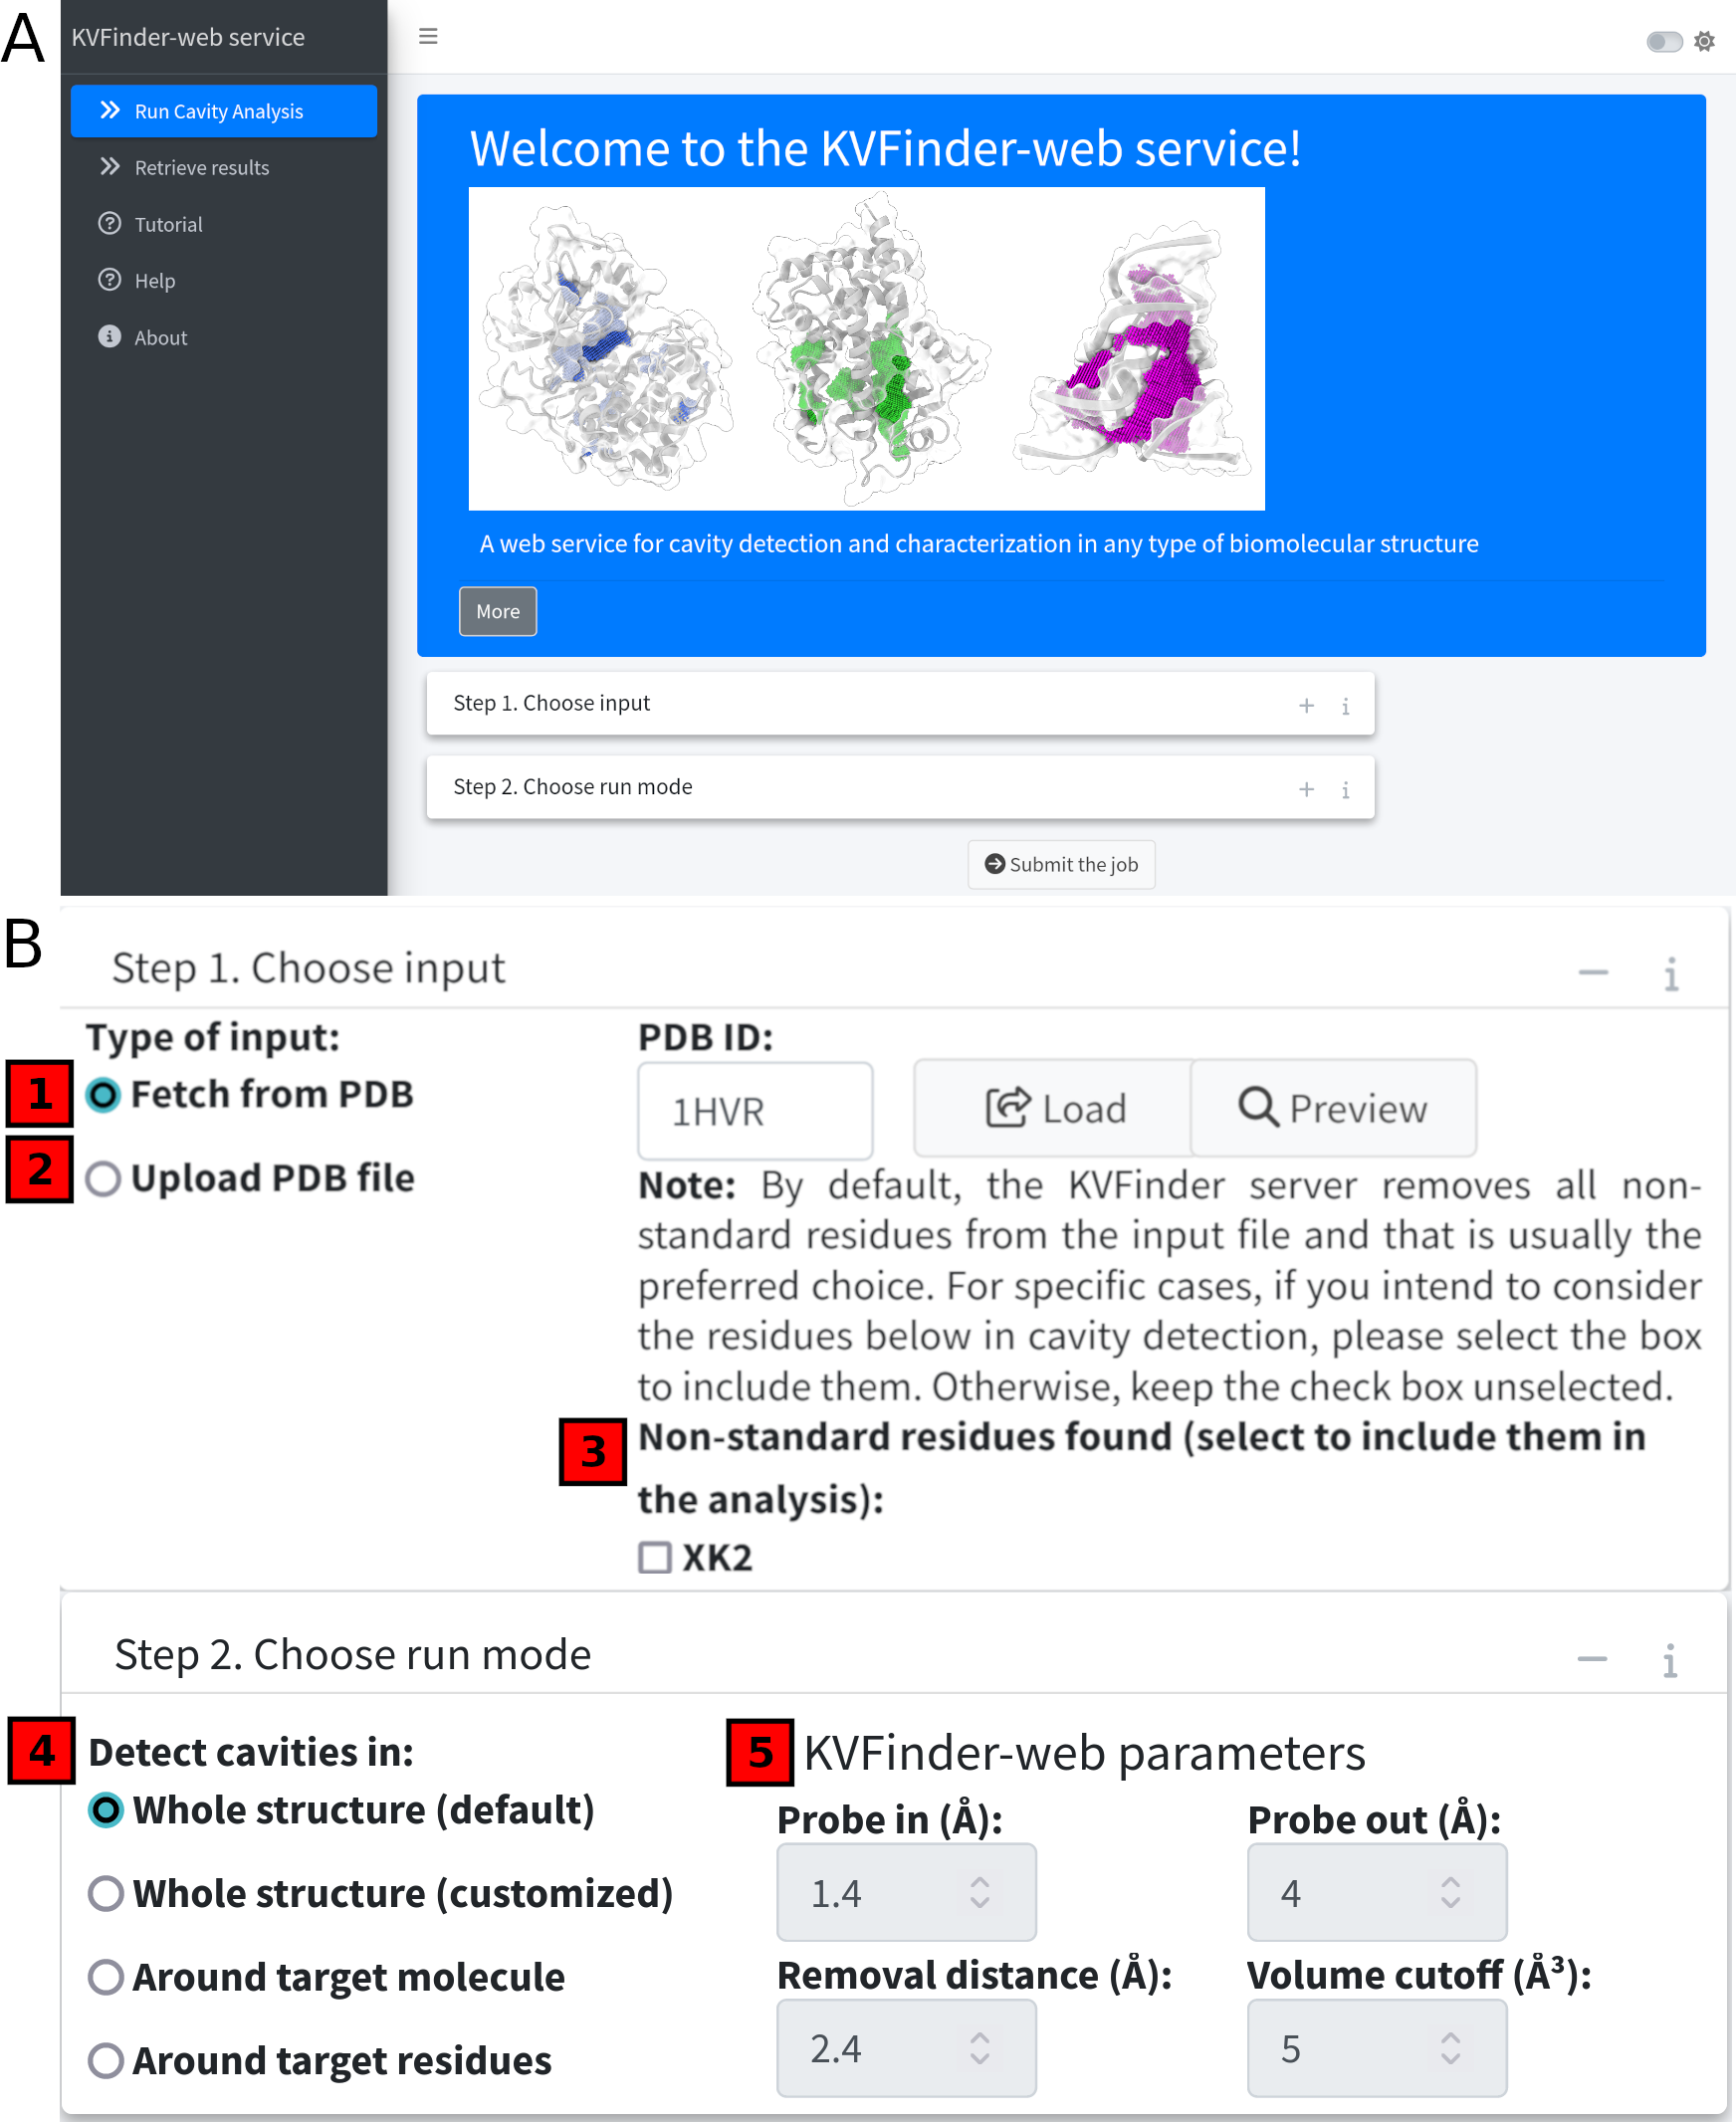
\includegraphics[scale=1.2]{images/kvweb-interface.png}
%   \centerline{\tiny{\textbf{Fonte:} Adaptado de \cite{guerra2023A}.}}
%   \caption[KVFinder-web portal]{\textbf{KVFinder-web portal.} \textbf{(A)} Página principal com as principais abas e as seções de entrada da biomolécula-alvo e escolha do modo de execução. \textbf{(B)} Visão detalhada de cada etapa que os usuários devem concluir antes de enviar a biomolécula-alvo para a análise da cavidade. A primeira etapa envolve a seleção da biomolécula-alvo, que pode ser feita fornecendo um ID do PDB e buscando no banco de dados do PDB (1) ou fazendo o upload de um arquivo PDB (2). Após o upload do PDB, o portal KVFinder-web verifica o PDB e informa sobre resíduos não padronizados detectados (3). Na próxima etapa, os usuários devem selecionar um modo de execução adequado (4) e personalizar, se necessário, os parâmetros de detecção (5).}
%   \label{fig:kvweb-interface}
% \end{figure}

% Os parâmetros personalizáveis de detecção incluem o \textit{Probe In}, o \textit{Probe Out}, o \textit{Removal Distance} e o \textit{Volume Cutoff} (Figura \ref{fig:kvweb-interface}B). Resumidamente, o \textit{Probe In} é uma sonda menor (em$\mAA$) que percorre a biomolécula-alvo, definindo sua superfície molecular (geralmente definida como uma esfera do tamanho de uma molécula de água - $1,4 \mAA$), enquanto o \textit{Probe Out} é uma sonda maior (em$\mAA$) que percorre a biomolécula-alvo, definindo regiões de inacessibilidade. Assim, as cavidades são definidas como as regiões acessíveis ao \textit{Probe In}, que normalmente são mais inclusivas, mas não ao \textit{Probe Out}. A \textit{Removal Distance} é uma distância (em$\mAA$) para remoção de pontos de cavidade a partir da fronteira cavidade-meio, a fim de delimitar os limites externos da cavidade. O \textit{Volume Cutoff} é um filtro de volume da cavidade (em$\mAA^3$) para excluir cavidades com volumes menores que esse limite, geralmente consideradas como cavidades sem relevância funcional. Para obter uma explicação mais detalhada de cada parâmetro, consulte as referências \cite{oliveira2014,guerra2019,guerra2020,guerra2021,guerra2023A}.
 
% Além disso, a interface gráfica permite aos usuários baixar e visualizar resultados de uma maneira fácil e interativa (Figura \ref{fig:kvweb-results}). As caracterizações morfológicas (volume, área e profundidade) e físico-químicas (hidrofobicidade) de cada cavidade são mostradas em uma tabela interativa, disponível para download no formato TOML. Um visualizador de biomoléculas, alimentado pelo motor gráfico NGL para R (NGLVieweR \cite{nglviewerr}), exibe a estrutura biomolecular com suas cavidades, para download no formato PDB, e permite várias personalizações, por exemplo, realçar cavidades e exibir resíduos de interface ao redor delas.

% \begin{figure}[h]
%   \centering
%   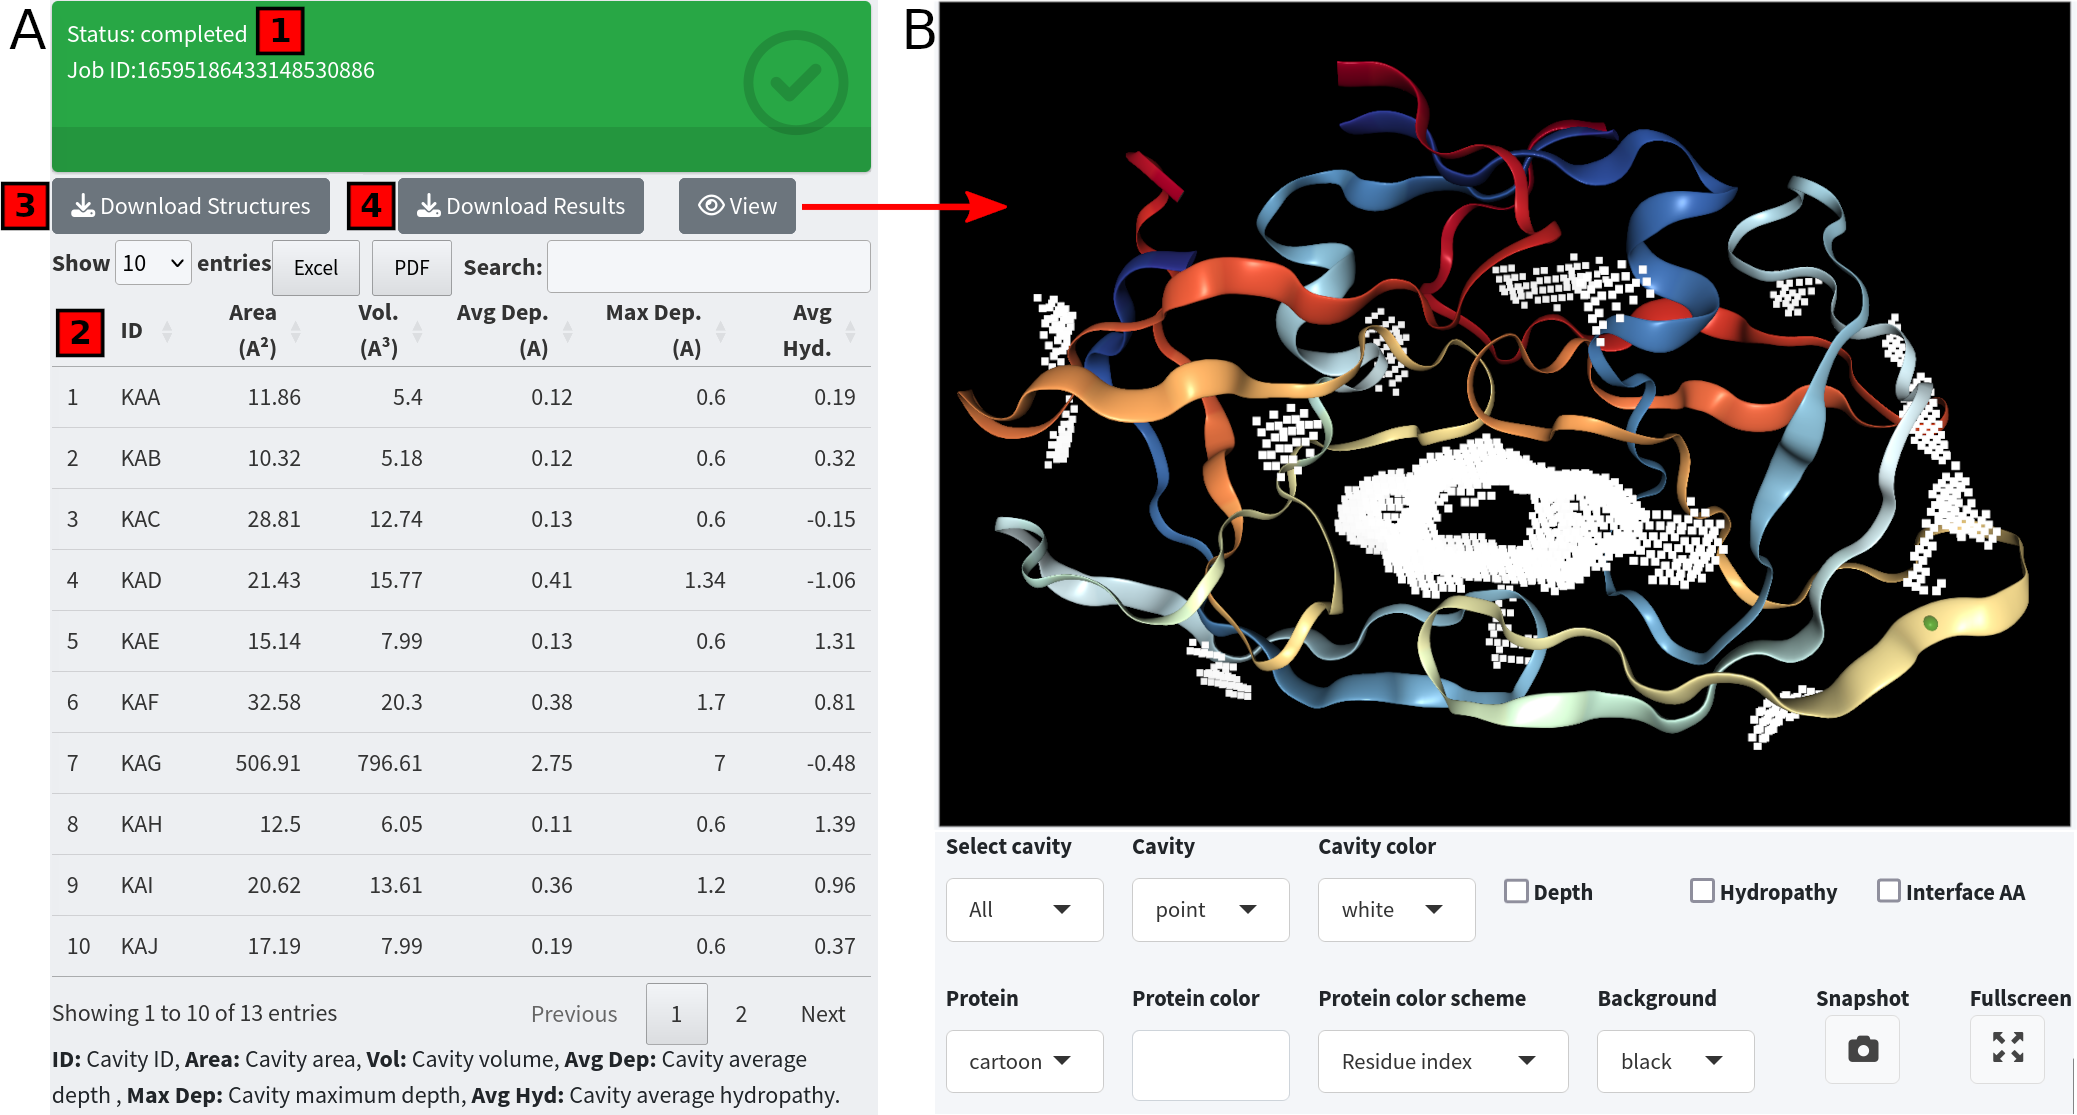
\includegraphics[scale=1.8]{images/kvweb-results.png}
%   \centerline{\tiny{\textbf{Fonte:} Adaptado de \cite{guerra2023A}.}}
%   \caption[Visualização de resultados no KVFinder-web portal]{\textbf{Visualização de resultados no KVFinder-web portal.} \textbf{(A)} Seção de resultados do KVFinder-web portal. A caixa de estado (verde: 'concluído'; amarelo: 'em execução' ou 'em fila'; vermelho: 'cancelado') do trabalho enviado (1). Após a conclusão, a interface apresenta os resultados em uma tabela, incluindo volume, área, profundidade média, profundidade máxima e hidropatia média das cavidades (2). Os usuários podem baixar um arquivo ZIP contendo a biomolécula-alvo e os arquivos PDB das cavidades (3) ou um arquivo TOML com a caracterização das cavidades (4). \textbf{(B)} A biomolécula-alvo com as cavidades pode ser visualizada ao clicar no botão 'Visualizar' e os usuários podem personalizar a visualização da biomolécula e das cavidades.}
%   \label{fig:kvweb-results}
% \end{figure}

% \subsection{KVFinder-web service}

% O \textbf{KVFinder-web service} é um serviço web RESTful que utiliza o parKVFinder (v1.2.0) para detectar e caracterizar cavidades em estruturas biomoleculares, conforme descrito em \cite{guerra2019,guerra2020,guerra2023A}. O serviço possui uma arquitetura Web-Fila-Trabalho (\textit{Web-Queue-Worker}, em inglês), que processa solicitações e respostas HTTP da interface web, gerencia os trabalhos e executa o parKVFinder nos trabalhos aceitos. A versão atual do KVFinder-web service é a \href{https://github.com/LBC-LNBio/KVFinder-web-service/tree/v1.1.0}{v1.1.0}. O código-fonte do KVFinder-web service está disponível no repositório: \url{https://github.com/LBC-LNBio/KVFinder-web-service}.

% \begin{figure}[H]
%   \centering
%   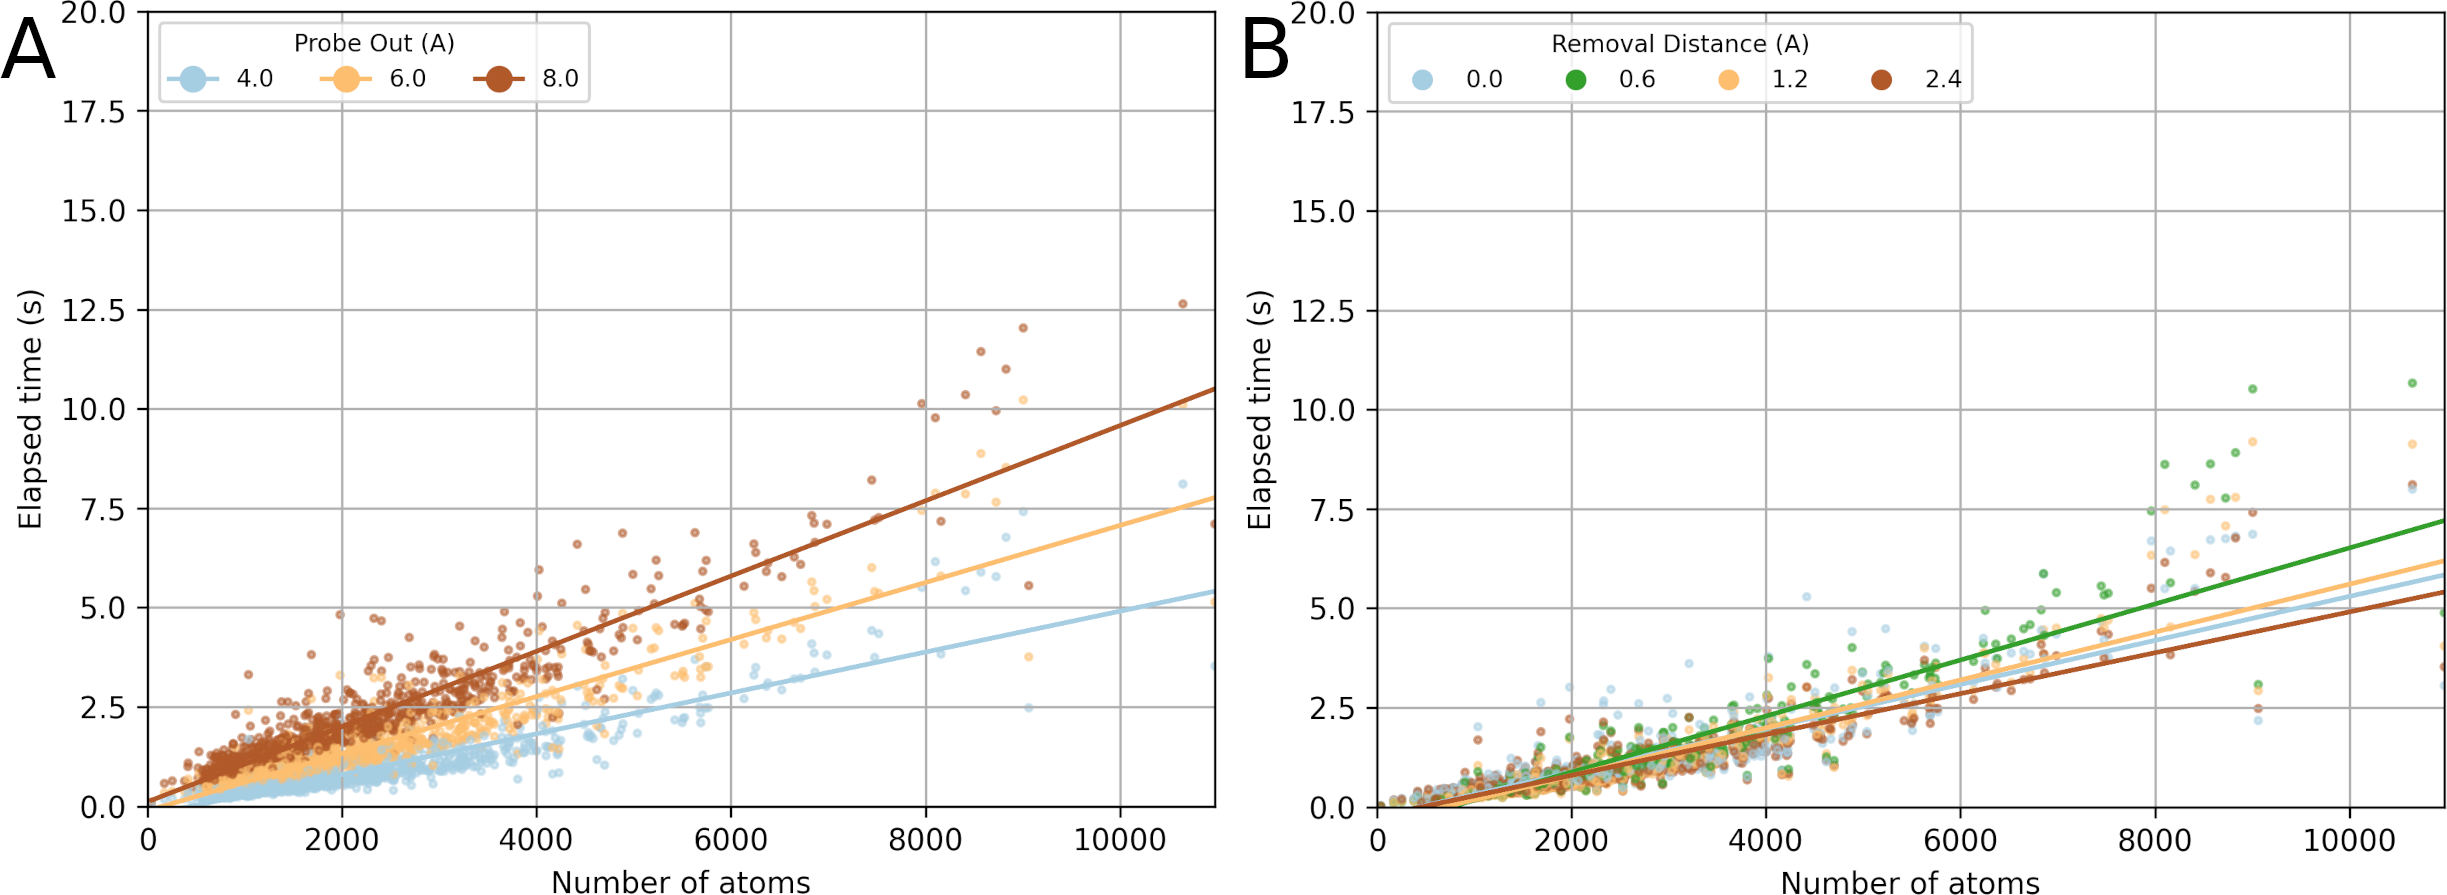
\includegraphics[scale=1.5]{images/kvweb-performance.png}
%   \centerline{\tiny{\textbf{Fonte:} Adaptado de \cite{guerra2023A}.}}
%   \caption[Efeitos dos parâmetros de detecção no desempenho do KVFinder-web service]{\textbf{Efeitos dos parâmetros de detecção no desempenho do KVFinder-web service.} A detecção de cavidades foi realizada no kv1000 \cite{guerra2020}, variando os parâmetros \textit{Probe Out} e \textit{Removal Distance}. O tempo decorrido em relação ao número de átomos na estrutura-alvo foi registrado, variando \textbf{(A)} os tamanhos do \textit{Probe Out} e \textbf{(B)} a \textit{Removal Distance}. Os cálculos foram realizados em um computador com processador AMD Ryzen 7 1700 de 8 núcleos e 3,0 GHz, 32GB de RAM, executando o sistema operacional Ubuntu 22.04 LTS.}
%   \label{fig:kvweb-performance}
% \end{figure}

% O KVFinder-web service utiliza uma arquitetura composta por três módulos: o \textit{Web server}, o \textit{Queue} e o \textit{Worker}. O módulo \textit{Web server}, desenvolvido em Rust usando o framework Actix (\url{https://actix.rs}), recebe as solicitações de trabalho no formato JSON via HTTP POST. Os dados recebidos devem conter as estruturas moleculares e os parâmetros de detecção do parKVFinder. Os trabalhos aceitos pelo módulo \textit{Web server} são enviados para o módulo \textit{Queue}, que é uma instância do servidor de fila de trabalhos Ocypod (\url{https://github.com/davechallis/ocypod}), onde aguardam para serem processados por um módulo \textit{Worker}. O módulo \textit{Worker} se comunica com o módulo \textit{Queue} e solicita o próximo trabalho a ser processado pelo parKVFinder. Após a conclusão do trabalho, a análise da cavidade (cavidades e suas caracterizações) é enviada de volta ao módulo \textit{Queue}, atualizando o status e os resultados do trabalho, que são disponibilizados aos clientes por meio do módulo \textit{Web server}. Para recuperar os resultados do trabalho, o cliente envia uma solicitação HTTP GET com o ID do trabalho, e o servidor web retorna o status atual do trabalho - 'em fila', 'em execução' ou 'concluído' - juntamente com os respectivos resultados, se disponíveis. Cada trabalho permanece armazenado em cache na fila por um dia após a conclusão. Como o ID do trabalho é criado aplicando uma função \textit{hash} nos dados recebidos, os resultados em cache são retornados quando a solicitação é reenviada. Cada módulo do KVFinder-web service é empacotado em um contêiner Docker \cite{docker}, tornando-o disponível para execução em ambientes locais ou de computação em nuvem. Esses módulos são combinados em um arquivo Docker Compose para facilitar a implantação.

% O desempenho computacional do KVFinder-web service também foi avaliado no kv1000 \cite{guerra2020}, variando dois parâmetros importantes relacionados à detecção de cavidades: \textit{Probe Out} e \textit{Removal Distance} (Figura \ref{fig:kvweb-performance}). A variação do parâmetro \textit{Probe Out} cria uma superfície molecular mais espessa ao redor da estrutura biomolecular, definindo a fronteira da cavidade. O aumento do valor do \textit{Probe Out} reduz a acessibilidade da superfície molecular e aumenta o tempo de cálculo no KVFinder-web service. Já o parâmetro \textit{Removal Distance} remove pontos da cavidade que estão próximos à fronteira, auxiliando na identificação de subcavidades e cavidades superficiais. O tempo de execução não apresenta uma relação clara com o parâmetro \textit{Removal Distance}, pois é influenciado pelo tamanho da fronteira e pelo número de cavidades, e não pelo número de átomos. De maneira geral, o tempo de execução aumenta de forma linear com o número de átomos na biomolécula-alvo dentro da grade 3D.

% \subsection{PyMOL KVFinder-web Tools}

% Para usuários familiarizados com o PyMOL \cite{pymol}, a ferramenta \textbf{PyMOL KVFinder-web Tools} (Figura \ref{fig:pymol-kvweb-tools}), desenvolvida em Python3 e Qt, integra o KVFinder-web service com o programa de visualização molecular. Essa interface gráfica de usuário (GUI; \textit{Graphical User Interface}, em inglês) amigável permite a personalização dos parâmetros de detecção para uma estrutura biomolecular-alvo e envia os trabalhos para um serviço KVFinder-web configurado (Figura \ref{fig:pymol-kvweb-tools}A). Atualmente, o PyMOL KVFinder-web Tools está na versão \href{https://github.com/LBC-LNBio/PyMOL-KVFinder-web-Tools/tree/v1.0.0}{v1.0.0}. O código-fonte do PyMOL KVFinder-web Tools está disponível no seguinte repositório: \url{https://github.com/LBC-LNBio/PyMOL-KVFinder-web-Tools}.

% \begin{figure}[H]
%   \centering
%   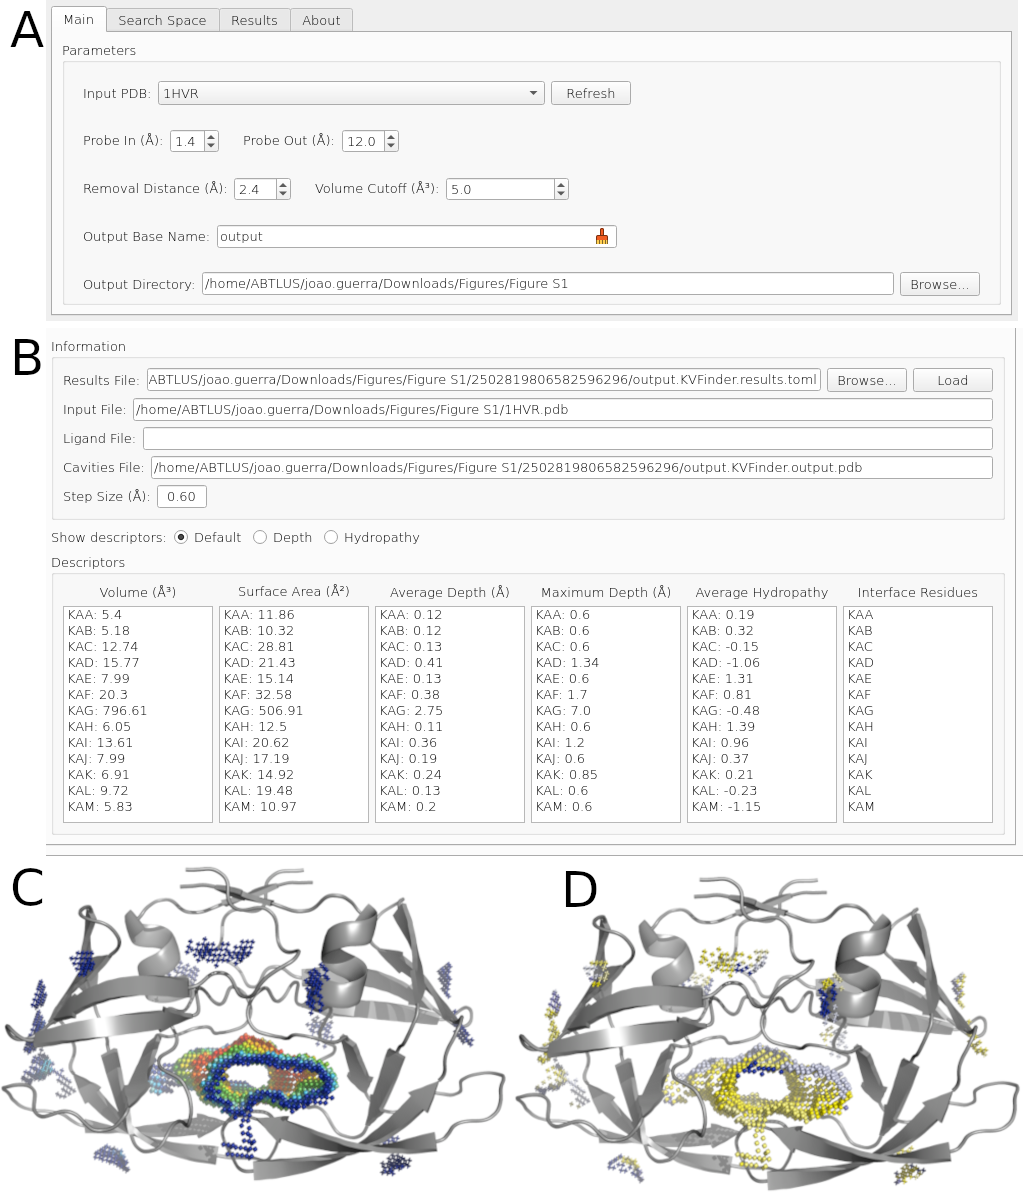
\includegraphics[scale=2.5]{images/pymol-kvweb-tools.png}
%   \centerline{\tiny{\textbf{Fonte:} Adaptado de \cite{guerra2023A}.}}
%   \caption[PyMOL KVFinder-web Tools]{\textbf{PyMOL KVFinder-web Tools.} Detecção de cavidades na estrutura da protease do HIV-1 (PDB ID: 1HVR), com \textit{Probe Out} definido como 12 Å. \textbf{(A)} Aba de parâmetros principais contendo parâmetros de detecção e estruturas moleculares a serem exploradas. \textbf{(B)} Aba de visualização contendo dados recebidos (cavidades e caracterizações) do serviço KVFinder-web exibidos na GUI. \textbf{(C)} Caracterização de profundidade e \textbf{(D)} caracterização de hidropatia de Eisenberg & Weiss, destacando o sítio ativo (cavidade KAG) na GUI e no visualizador do PyMOL.}
%   \label{fig:pymol-kvweb-tools}
% \end{figure}

% Assim como no plugin parKVFinder para PyMOL \cite{guerra2020}, o espaço de busca também pode ser ajustado para uma caixa personalizada (\textit{box adjustment mode}) e/ou um raio ao redor de um ligante ou molécula-alvo (\textit{ligand adjustment mode}), em vez de detectar e caracterizar cavidades em toda a superfície biomolecular (\textit{whole protein mode}). Após o envio bem-sucedido, os trabalhos aceitos são solicitados rotineira e assincronamente ao KVFinder-web service. Quando um trabalho é concluído, o plugin processa automaticamente os dados recebidos, cavidades e caracterizações, para arquivos locais e os disponibiliza na GUI. Esse plugin gráfico opera de maneira semelhante ao KVFinder-web portal, as caracterizações são mostradas em listas (Figura \ref{fig:pymol-kvweb-tools}B) e as cavidades são personalizadas por suas propriedades no visualizador do PyMOL (Figura \ref{fig:pymol-kvweb-tools}C e D). No entanto, os trabalhos enviados no KVFinder-web portal podem ser carregados no PyMOL KVFinder-web Tools e vice-versa.

% \subsection{Caso de estudo}

% O KVFinder-web foi aplicado em dois casos de estudo publicados em periódico científico para investigar proteínas de interesse terapêutico. Essas análises exploraram a caracterização do sítio catalítico da protease do vírus da imunodeficiência humana tipo 1 (HIV-1) e a comparação morfológica das estruturas desta proteína depositadas no wwPDB. No apêndice \ref{ap:casos-de-estudo-kvfinder-web}, descreveremos cada um desses casos de estudo em detalhes.

% \subsection{Discussão}

% Em linhas gerais, a disponibilização do KVFinder-web visa ampliar o uso dessa robusta ferramenta de detecção de cavidades na comunidade científica. Além disso, o KVFinder-web tem o propósito de democratizar a ferramenta parKVFinder e remover as barreiras para usuários que não possuem conhecimento técnico para instalar e configurar um ferramenta computacional de detecção de cavidades, que possuem recursos computacionais limitados ou que desejam realizar uma análise simples e rápida. Isso simplificará o processo de detecção e caracterização de cavidades, mesmo para usuários menos experientes, com impacto direto no busca e desenho racional de fármacos e na compreensão das estruturas de biomoléculas.

\section{SERD \label{sec:serd}}

% Reescrever:
% 1 - estudo de acessibilidade
% 2 - representação de estruturas biomoleculares na forma de grafos
% 3 - cavidades também é possível

% A teoria de grafos tem sido relevante tanto no campo da biologia quanto nas ciências farmacêuticas, sendo aplicada no estudo da estrutura, função e evolução de proteínas, bem como em análises de DM e redes de interação receptor-ligante \cite{vishveshwara2002,mason2007,hummer2023}. Conforme apresentado em \cite{hummer2023}, as representações de complexos proteína-proteína (\ie, complexos anticorpo-antígeno) podem ser aplicadas em técnicas de aprendizado profundo (\textit{deep learning}, em inglês) para prever $\Delta \Delta G$ experimental. Além disso, as representações em forma de grafo podem ser utilizadas em uma ampla gama de técnicas de aprendizado de máquina e ciência de dados, conforme ilustrado na Seção \ref{sec:graph-representation} e discutido em estudos anteriores \cite{majeed2020,vishveshwara2002,mason2007}. Neste cenário, desenvolvemos o \textbf{SERD}, uma ferramenta para representação de estruturas biomoleculares na forma de grafos, desde sítios de ligação (\eg, cavidades identificadas pelo KVFinder suite) até complexos biomoleculares (\eg, IPPs, IPLs, IPRs e IPDs), conforme ilustrado na Figura \ref{fig:serd-graph}. Atualmente, o SERD está na versão \href{https://github.com/jvsguerra/SERD/tree/v0.1.2}{v0.1.2}. O código-fonte do SERD está disponível no seguinte repositório: \url{https://github.com/jvsguerra/SERD}.

% Além disso, sabe-se que o reconhecimento molecular depende diretamente da acessibilidade de um ligante ao sítios de ligação do seu respectivo receptor. Os resíduos expostos ao solvente de uma biomolécula-alvo (receptor) compõe o conjunto de átomos acessíveis a possíveis ligantes. Nesse contexto, a identificação desses resíduos possibilita um estudo mais direcionado aos \textit{hotspots} de interação de um receptor-alvo, com aplicações principalmente no estudo de acoplamento molecular (\eg, \textit{docking} proteína-proteína e \textit{docking} proteína-ligante). No SERD, também implementamos um algoritmo para identificar resíduos expostos ao solvente em uma biomolécula-alvo. Essa abordagem aproxima uma molécula de solvente a uma sonda esférica, que escaneia a superfície do receptor alvo para identificar as regiões (\ie, resíduos) que são acessíveis a esta sonda esférica, de forma semelhante ao escaneamento da grade 3D da sonda \textit{Probe Out} no KVFinder suite \ref{fig:parkvfinder-schema}. Após a identificação desses resíduos, a ferramenta os representa na forma de grafos pela biblioteca NetworkX \cite{networkx}, formando arestas até uma distância limite entre \acs{CA}, \acs{CB} ou quaisquer átomos do resíduo e opcionalmente incluir essas distâncias como atributos das arestas desses grafos. Opcionalmente, essas distâncias podem ser incluídas como atributos das arestas desses grafos, conforme ilustrado na Figura \ref{fig:serd-graph}B.

% Por fim, esta ferramenta é aplicada em duas colaborações do Laboratório de Biologia Computacional: o projeto de Mestrado do aluno Marcos Rogério Simões do PPGCF/FCF, intitulado "Descrição e caracterização de sítios de ligação através de teoria dos grafos", para estudar a similaridade entre sítios de ligação entre famílias de quinases, e o projeto de pesquisa do Dr. Gabriel Ernesto Jara para estudo de complexos anticorpo-antígeno através de fragmentos da superfície.

\section{KVFinderMD}

% Em algumas circunstâncias, para a formação do complexo receptor-ligante, os receptores utilizam sítios de ligação que não são facilmente identificados na forma não-ligada. Algumas interações biomoleculares (\eg, IPPs, IPLs, IPRs and IPDs) dependem da dinâmica intrínseca do receptor-alvo, nas quais o modelo clássico de chave-fechadura falha e modelos mais recentes de ligação, como ajuste induzido e seleção conformacional, são aplicáveis \cite{holyoak2013}. Nesse sentido, as simulações de DM são uma ferramenta útil para entender os mecanismos de reconhecimento molecular e, em última análise, a função biomolecular. Recentemente, desenvolvemos o pyKVFinder \cite{guerra2021} como um bloco de construção para aplicações mais complexas, como análises de simulações de DM. Utilizando-o como base, desenvolvemos uma nova ferramenta chamada \textbf{KVFinder for Molecular Dynamics analysis (KVFinderMD)}, um pacote em Python que permite explorar a dinâmica dos sítios de ligação em estruturas biomoleculares de interesse farmacológico. Uma vez que a dinâmica intrínseca da biomolécula pode alterar a forma e as propriedades do sítio de ligação ao longo do tempo, o KVFinderMD caracteriza cavidades em relação ao volume, área, profundidade, hidropatia e resíduos de interface, que são propriedades relevantes para descrever o processo de reconhecimento molecular (Figura \ref{fig:kvmd-overview}A). 

% \begin{figure}[h]
%   \centering
%   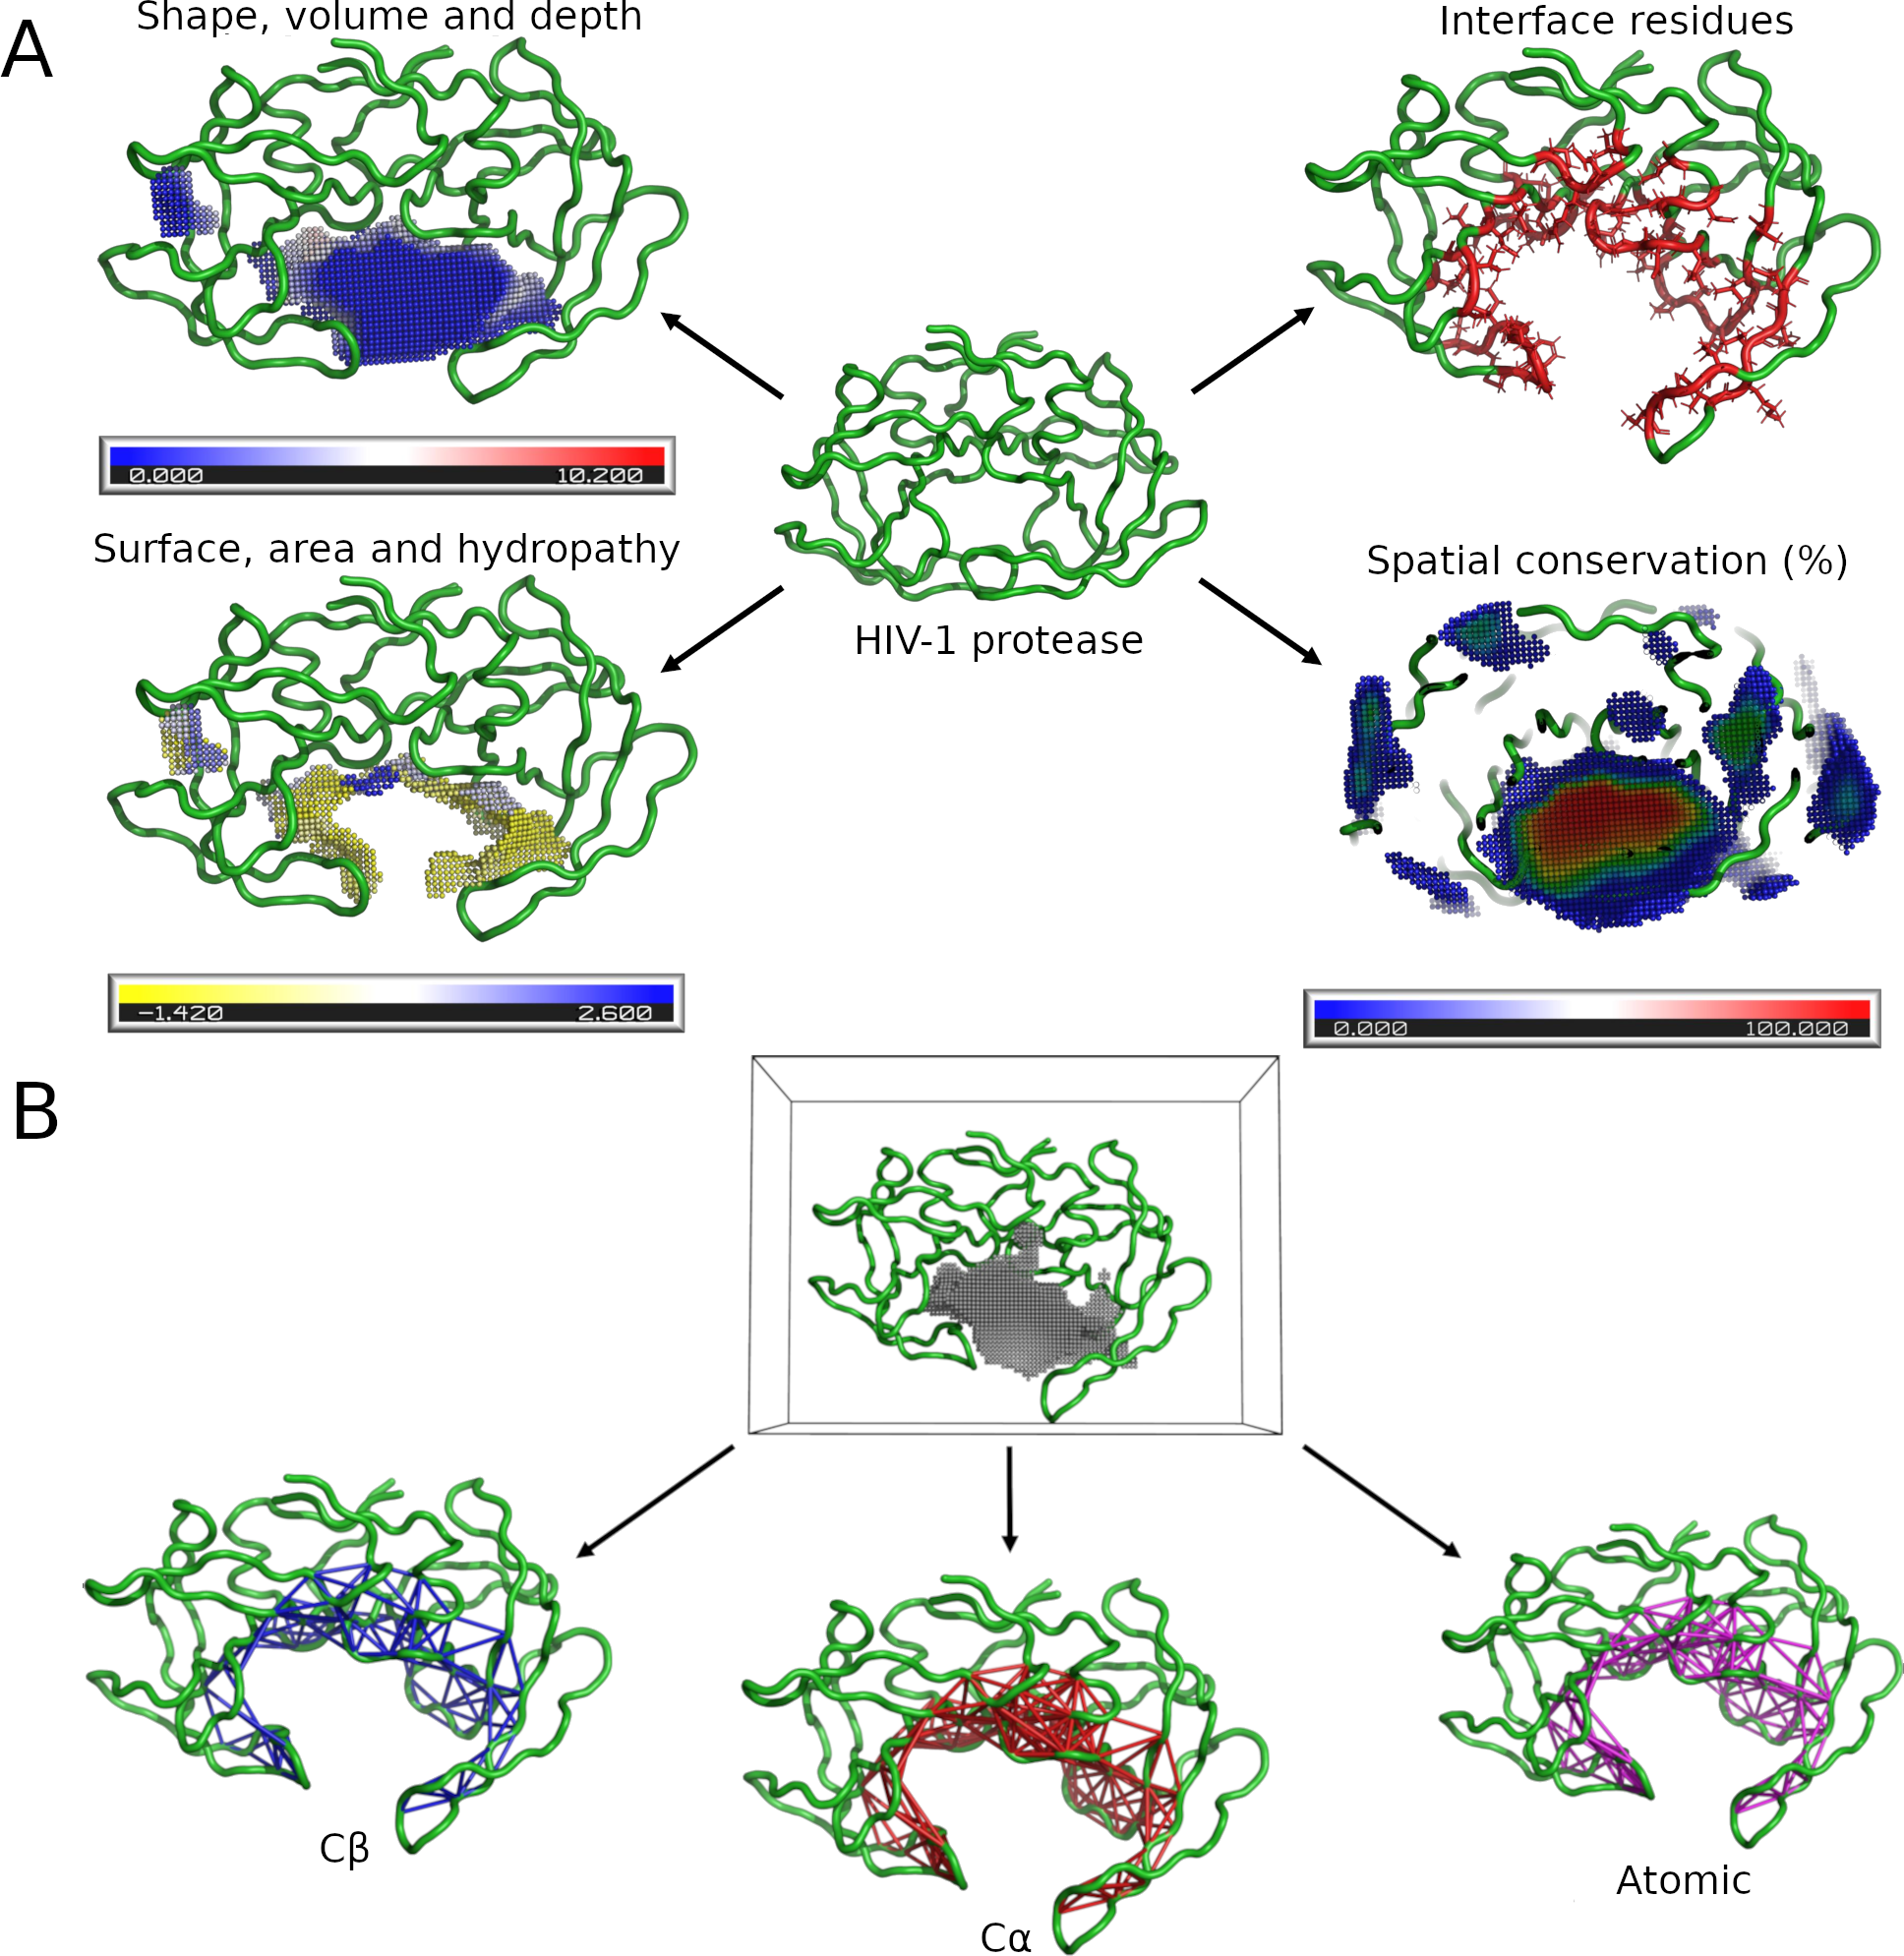
\includegraphics[scale=0.8]{images/kvmd-overview.png}
%   \caption[Detecção, caracterizações e representações de cavidades em estudos de dinâmica molecular usando a ferramenta KVFinderMD]{\textbf{Detecção, caracterizações e representações de cavidades em estudos de dinâmica molecular usando a ferramenta KVFinderMD.} \textbf{(A)} Caracterizações morfológicas, topológicas e físico-químicas aplicadas no KVFinderMD. \textbf{(B)} Representação em forma de grafo das cavidades baseada nos resíduos de interface e suas relações topológicas. Distância entre \acs{CB} (azul), \acs{CA} (vermelho) e quaisquer átomos de um resíduo (magenta).}
%   \label{fig:kvmd-overview}
% \end{figure}

% Para a leitura de dados binários gerados por programas de simulação de DM, como GROMACS \cite{gromacs}, AMBER \cite{amber} e CafeMol \cite{kenzaki2011}, utilizamos o pacote MDAnalysis \cite{mdanalysis} para integrar a leitura e processamento dos arquivos de trajetória de DM (\eg, GRO, CRD, NC, DCD, XTC/TRR) e os arquivos de topologia (\eg, PSF, PRMTOP, GRO, PDB) no KVFinderMD. Adicionalmente, implementamos um protocolo para a análise de conservação de cavidades ao longo da DM (Figura \ref{fig:kvmd-overview}A; quadro inferior direito), similar ao apresentado na análise de conservação do sítio de ligação do ADP-ribose no domínio ADRP do SARS-CoV-2 e proteínas relacionadas (Figura \ref{fig:conservation-analysis}). Por fim, também integramos a representação em forma de grafos, implementada no SERD (veja Seções \ref{sec:graph-representation} e \ref{sec:serd}), que considera distâncias carbono \textalpha, carbono \textbeta\space ou quaisquer átomos, para descrever o sítio de ligação (Figura \ref{fig:kvmd-overview}B). Desta forma, a similaridade das cavidades pode ser determinada a partir do agrupamento hierárquico das representações de grade 3D, topológica e em forma de grafos das cavidades, permitindo acompanhar as cavidades ao longo da DM.

% \subsection{Caso de estudo}

% % O KVFinderMD foi aplicado em dois casos de estudo para investigar proteínas de interesse terapêutico. Essas análises exploraram a similaridade de cavidades da protease da HIV-1 ao longo de uma simulação de DM e a caracterização dos sítios de ligação do substrato de ALDH1 e ALDH2. Ambos casos de estudo foram apresentados em detalhe no IV Congresso de Estudantes do CNPEM (IV CEC), realizado entre 22 e 24 de novembro de 2022, e recebeu prêmio pela apresentação intitulada "KVFinderMD: a Python package to detect and describe binding sites in molecular dynamics trajectories".

% O KVFinderMD foi aplicado em um caso de estudo para explorar a similaridade de cavidades da protease da HIV-1 ao longo de uma simulação de DM. Este caso de estudo foi apresentado em detalhe no IV Congresso de Estudantes do CNPEM (IV CEC), realizado entre 22 e 24 de novembro de 2022, e recebeu prêmio pela apresentação intitulada "KVFinderMD: a Python package to detect and describe binding sites in molecular dynamics trajectories".

% \subsubsection{Similaridade de cavidades da HIV-1 protease ao longo de uma simulação de dinâmica molecular}

% Partindo da DM da HIV-1 protease, onde descrevemos com sucesso as alterações conformacionais que definem o sítio ativo (veja Seção \ref{sec:md-hiv1-protease}), aplicamos um alinhamento estrutural das cavidades, usando representações em grade 3D, representação topológica e representação em grafos, da protease do HIV-1 ao longo da simulação de DM. Com as três representações de cavidades implementadas no KVFinder suite, exploramos algoritmos de agrupamento não-supervisionados, onde o agrupamento hierárquico apresentou os melhores resultados, além de fornecer uma relação de similaridade entre as cavidades. Além disso, exploramos diferentes métricas de afinidade para agrupar as cavidades ao longo da trajetória da HIV-1 protease.

% Para realizar o agrupamento, separamos cada cavidade em uma estrutura de dados individual e adaptamos a codificação dos dados de sítios de ligação (Figura \ref{fig:hiv-1-representation}). Na representação de grade 3D, transformamos os valores armazenados em booleanos, onde os pontos de cavidades são marcados com o valor 1, enquanto os demais pontos recebem o valor 0. Na representação topológica, transformamos os valores em uma matriz quadrada de distâncias entre os resíduos, ordenados de acordo com a sequência da proteína. Por fim, na representação em grafo, transformamos os valores em uma matriz quadrada de contatos entre os resíduos, também ordenados de acordo com a sequência da proteína. Para isso, utilizamos a distância entre os átomos de \acs{CB} dos resíduos, com o corte de distância de 8 \AA para definir os contatos, que é a métrica padrão do SERD.

% \begin{figure}[h]
%   \centering
%   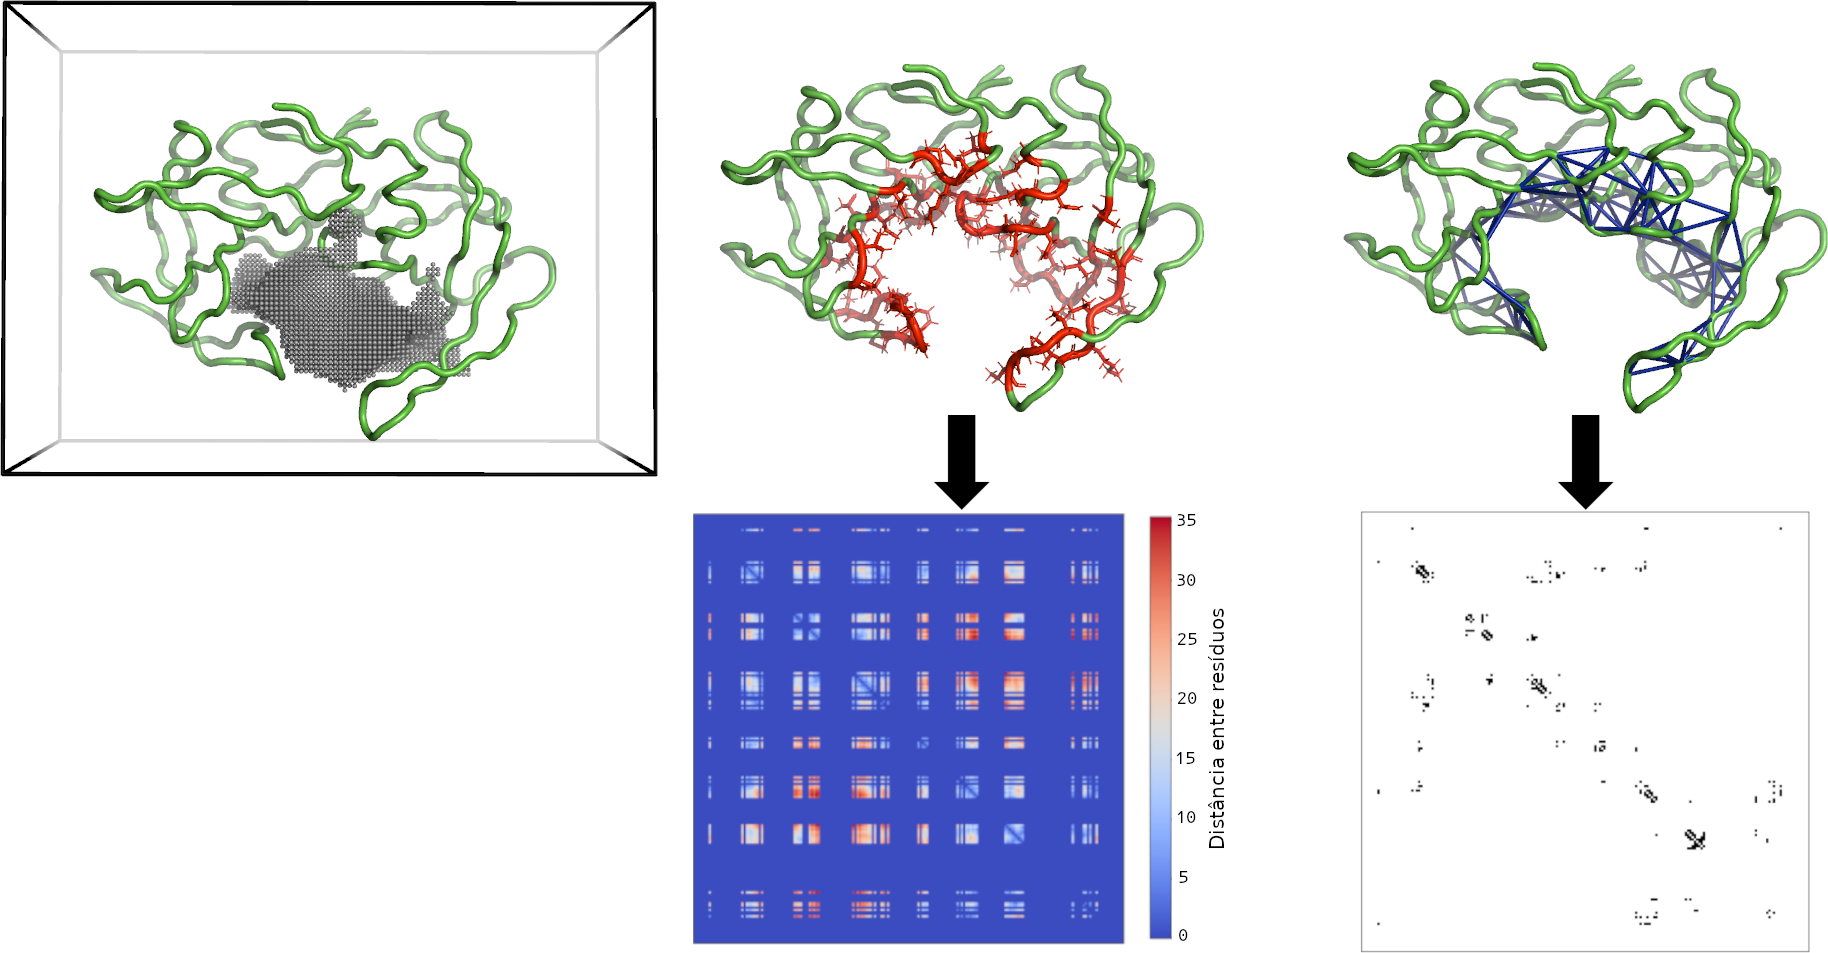
\includegraphics[scale=1]{images/HIV-1-representation.png}
%   \caption[Codificação de dados para estudo de similaridade de cavidades da HIV-1 protease ao longo da trajetória de dinâmica molecular]{\textbf{Codificação de dados para estudo de similaridade de cavidades da HIV-1 protease ao longo da trajetória de dinâmica molecular.} Representação da cavidade do sítio ativo em grade 3D (quadro esquerdo), onde os pontos de cavidade são identificado por 1, enquanto os demais pontos (pontos de biomolécula, pontos de meio e pontos de espaço vazio) identificados o valor 0. Representação topológica do sítio ativo (quadro central), onde abstraímos as cavidades como um matriz de distância, ordenados pela sequência da proteína. Representação em forma de grafo das relações entre os resíduos do sítio ativo (quadro direito), onde abstraímos as cavidades como um matriz de contatos, ordenados pela sequência da proteína.}
%   \label{fig:hiv-1-representation}
% \end{figure}

% Nesse caso de estudo, detectamos 672 cavidades ao longo dos 201 quadros de simulação, \ie, teremos 672 estruturas de dados a serem agrupadas por agrupamento hierárquico, explorando as métricas de afinidade apropriadas para cada representação. Para vetores booleanos, avaliamos as seguintes métricas disponíveis no pacote SciPy \cite{scipy}: dissimilaridade de Dice ($d_{Dice}$; Equação \ref{eq:dice}), distância de Hamming, dissimilaridade de Jaccard-Needham, dissimilaridade de Kulczynski, dissimilaridade de Rogers-Tanimoto, dissimilaridade de Russell-Rao, dissimilaridade de Sokal-Michener, dissimilaridade de Sokal-Sneath e dissimilaridade de Yule. Para vetores numéricos, avaliamos as seguintes métricas disponíveis no pacote SciPy \cite{scipy}: distância de correlação ($\rho$; Equação \ref{eq:correlacao}), distância de Bray-Curtis, distância de Canberra, distância Chebyshev, distância de Manhattan (também conhecido como distância de \textit{City Block}), distância de Cosseno ($d_{Cosseno}$; Equação \ref{eq:cosseno}), distância de Jensen-Shannon e distância quadrática Euclidiana. 

% \begin{equation}
%   d_{\sf dice} \colon (u,v) \mapsto \frac{C_{VF}(u,v) + C_{FV}(u,v)}{2 C_{VV}(u,v) + C_{VF}(u,v) + C_{FV}(u,v)} \in [0,1]
%   \label{eq:dice}
% \end{equation}

% \noindent onde $C_{ij}$ é o número de ocorrências de $u[k] = i$ e $v[k] = j$ para $k<n$.

% \begin{equation}
%   \rho(u,v) = 1 - \frac{(u - \bar{u}) \cdot (v - \bar{v})}{{\|(u - \bar{u})\|}_2 {\|(v - \bar{v})\|}_2}, \rho \in [-1, 1],
%   \label{eq:correlacao}
% \end{equation}

% \noindent onde $\bar{u}$ é a média dos elementos de $u$, $\bar{v}$ é a média dos elementos de $v$, e $x \cdot y$ é o produtor escalar de $x$ e $y$.

% \begin{equation}
%   d_{Cosseno}(u,v) = 1 - \frac{u \cdot v}{\|u\|_2 \|v\|_2}, d_{Cosseno} \in [-1, 1],
%   \label{eq:cosseno}
% \end{equation}

% \noindent onde $u \cdot v$ é o produtor escalar de $u$ e $v$.

% Como não existe um verdade absoluta para o agrupamento das cavidades, utilizamos o Coeficiente de Silhueta (\textit{Silhouette Score}, em inglês; Equação \ref{eq:silhouette-score}) para maximizar a semelhança entre membros de um grupo e a diferença entre membros de grupos distintos, onde o melhor valor é 1, o pior é -1 e 0 indica agrupamentos sobrepostos. Assim, valores negativos geralmente indicam que uma amostra está no grupo errado, já que um grupo diferente é mais similar à amostra do que o grupo que ela está atribuída. Por fim, é importante destacar que os coeficientes de silhueta não podem ser comparados entre diferentes métricas de afinidade. Portanto, comparamos os métodos com base no número ideal de grupos identificados pelo coeficiente de silhueta máximo dentro de uma mesma métrica de afinidade.

% \begin{equation}
%   Coeficiente\;de\;Silhueta = \frac{(b - a)}{max(a, b)}, Coeficiente\;de\;Silhueta \in [-1, 1],
%   \label{eq:silhouette-score}
% \end{equation}

% onde $a$ é a distância média intra-cluster e $b$ é a distância para o cluster mais próximo para cada amostra.

% Em seguida, aplicamos o algoritmo de agrupamento hierárquico não supervisionado, otimizando o coeficiente de silhueta para cada métrica de afinidade, utilizando o método de ligação completo (Figura \ref{fig:hiv-1-clustering-results}). Para a representação em grade 3D, não exploramos diferentes métricas de afinidade devido ao tamanho dos dados ($\aproximadamente 10^6$ pontos por cavidade), e portanto, utilizamos a distância de correlação (Equação \ref{eq:correlacao}), onde encontramos 10 grupos com um coeficiente de silhueta máximo de $\aproximadamente 0{,}42$. Com a simplificação do tamanho dos dados para as duas representações restantes ($\aproximadamente 10^4$ pontos por cavidade), foi possível explorar as métricas de afinidade apropriadas. Para a representação topológica, a distância de cosseno (Equação \ref{eq:cosseno}) apresentou o maior número de grupos entre as métricas numéricas (\ie, 15 grupos) com um coeficiente de silhueta máximo de $\aproximadamente 0{,}54$. Para a representação em forma de grafo, a dissimilaridade de Dice (Equação \ref{eq:dice}) apresentou o maior número de grupos entre as métricas numéricas (\ie, 16 grupos) com um coeficiente de silhueta máximo de $\aproximadamente 0{,}52$.

% \begin{figure}[h]
%   \centering
%   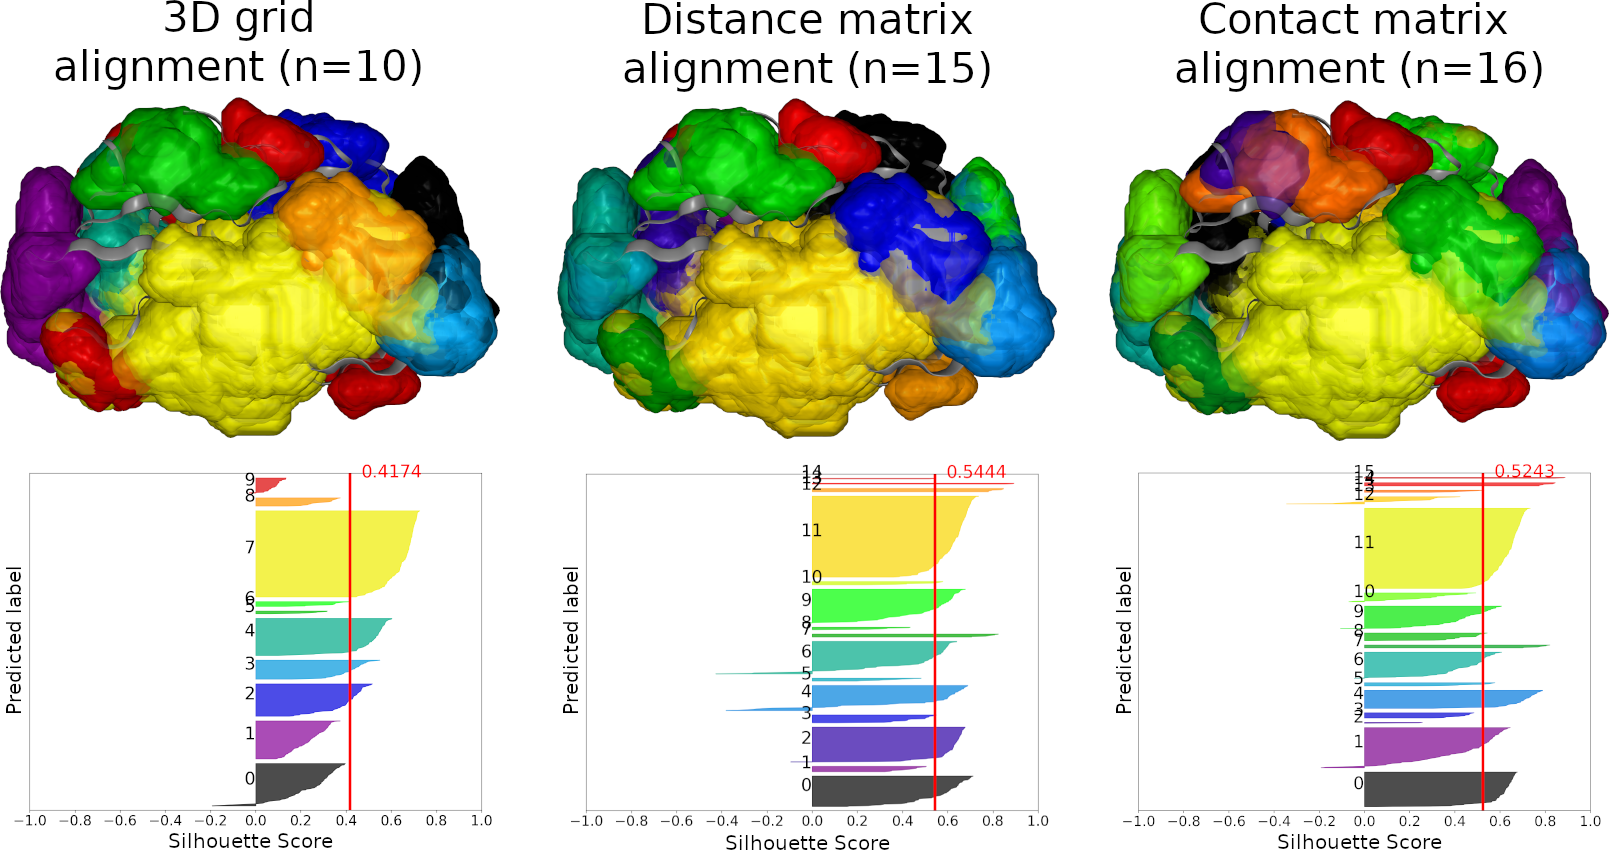
\includegraphics[scale=1.1]{images/HIV-1-clustering-results.png}
%   \caption[Agrupamento hierárquico das cavidades da protease do HIV-1]{\textbf{Agrupamento hierárquico das cavidades da protease do HIV-1.} Todas as cavidades detectadas ao longo da dinâmica molecular foram sobrepostas na mesma estrutura e coloridas de acordo com os rótulos atribuídos pelo agrupamento hierárquico da grade 3D (quadro esquerdo), da matriz de distâncias (quadro central) e da matriz de contatos (quadro direito). O gráfico de coeficiente de silhueta é apresentado para cada amostra de acordo com o rótulo atribuído. A linha vermelha indica o valor do coeficiente de silhueta médio para o agrupamento hierárquico.}
%   \label{fig:hiv-1-clustering-results}
% \end{figure}

% A partir desses agrupamentos, conseguimos agrupar com sucesso as cavidades e acompanhar a evolução delas ao longo da simulação de DM. Isso simplificou a comparação das características entre as cavidades ao longo do tempo. O uso das matrizes de distância e matrizes de contatos mostrou-se efetivo devido à sua capacidade de agrupar as cavidades. Além disso, essas representações foram mais rápidas e simples para agrupar as cavidades ao longo do tempo em simulações de DM, já que o algoritmo de agrupamento hierárquico tem uma complexidade de aproximadamente $\mathcal{O}(n^3)$ e o tamanho dos dados diminui em 100 vezes por cavidade em comparação com a estrutura original. Portanto, considerando que temos 672 cavidades nesse caso de estudo, a redução do uso de memória é de aproximadamente 67200 vezes.

% \subsection{Discussão}

% A aplicação do KVFinderMD ilustra a integração das ferramentas disponíveis no KVFinder suite (\ie, pyKVFinder e SERD) para realizar uma análise sistemática de cavidades por meio de um protocolo automatizado. Ao utilizar algoritmos de agrupamento hierárquico e diferentes métricas de afinidade em várias representações (grade 3D, representação topológica e representação em grafo), pudemos identificar grupos de cavidades mais similares, o que nos permitiu avaliar a evolução temporal dos sítios de ligação. Além disso, conseguimos reduzir o tamanho dos dados necessários para a análise e simplificar a comparação entre as cavidades em simulações de DM, demonstrando uma aplicabilidade prática do KVFinder suite.

% A análise da similaridade das cavidades da protease do HIV-1 ao longo da simulação de DM nos permitiu acompanhar a evolução dessas cavidades e comparar suas características ao longo do tempo, como apresentado na Figura \ref{fig:hiv1-protease-dm-analysis}. Isso foi realizado sem interferência humana, utilizando os recursos automatizados do KVFinderMD. No entanto, é importante ressaltar que, embora o KVFinderMD seja uma ferramenta útil para a análise de cavidades em simulações de DM, existem algumas limitações a serem consideradas. Por exemplo, a escolha das métricas de afinidade e dos parâmetros de agrupamento hierárquico pode influenciar os resultados obtidos. Portanto, é fundamental realizar uma avaliação cuidadosa e explorar diferentes configurações para obter os melhores resultados. % Além disso, a detecção de cavidades em simulações de DM depende da precisão e qualidade das estruturas conformacionais geradas durante a simulação. Variações conformacionais insuficientes podem levar à detecção de cavidades menos representativas ou à perda de informações importantes. Portanto, é necessário considerar esses aspectos ao interpretar os resultados obtidos com o KVFinderMD.

% Apesar dessas limitações, o KVFinderMD representa um avanço significativo no estudo das interações biomoleculares ao longo do tempo. Sua capacidade de automatizar a análise de cavidades em simulações de DM, combinada com as outras ferramentas do KVFinder suite, oferece uma abordagem abrangente para investigar os sítios de ligação e compreender sua evolução. Isso pode ser útil no desenvolvimento de estratégias terapêuticas e no desenho racional de novos fármacos, especialmente em sítios de ligação transientes.

\section{Benchmarking of Well-established Cavity Detection Tools}
% \section{\textit{Benchmarking} das ferramentas disponíveis}

% %%% Chapter 5

% \chapter{Conclusão}

% Após estudo cuidadoso das demandas de ferramentas computacionais da comunidade de biologia estrutural, desenvolvemos com sucesso a plataforma computacional KVFinder suite. Essa plataforma foi projetada para estudos de sistemas biomoleculares, fornecendo ferramentas abrangentes de codificação e caracterização de biomoléculas e seus sítios de ligação. O KVFinder suite é composto por 5 ferramentas computacionais, englobando diferentes demandas e objetivos da comunidade de biologia estrutural, que são o KVFinder-web, parKVFinder, pyKVFinder, SERD e KVFinderMD. 

% O KVFinder-web é uma aplicação web de código aberto para detecção e caracterização de cavidades, usando o parKVFinder, em qualquer tipo de estrutura biomolecular. O KVFinder-web visa ampliar o uso do parKVFinder na comunidade científica, além de democratizar o acesso e remover barreiras para usuários que não possuem conhecimento técnico para instalar e configurar uma ferramenta computacional, que possuem recursos computacionais limitados ou que desejam realizar uma análise simples e rápida. A aplicação web está disponível em \url{https://kvfinder-web.cnpem.br}.

% O parKVFinder é uma ferramenta de código aberto desenvolvida para a detecção e caracterização de cavidades biomoleculares. Ele inclui um plugin gráfico integrado ao visualizador molecular PyMOL, que oferece uma interface intuitiva para explorar parâmetros personalizáveis e visualizar as cavidades detectadas e suas características. Embora o parKVFinder tenha limitações em aplicações automatizadas e comparações sistemáticas de sítios de ligação, ele desempenha um papel importante na otimização dos parâmetros de detecção e caracterização por meio do plugin gráfico do PyMOL (PyMOL2 parKVFinder Tools), devido aos seus recursos visuais. Estes parâmetros otimizados podem ser posteriormente adotados em estudos automatizados e comparações sistemáticas de sítios de ligação.

% O pyKVFinder é um pacote Python de código aberto para detectar e caracterizar cavidades em estruturas biomoleculares em protocolos automatizados e aplicações de ciência de dados. Além de possuir as mesmas funcionalidades do KVFinder-web e parKVFinder, o pyKVFinder fornece estruturas de dados acessíveis e flexíveis no ecossistema Python, como \textit{ndarrays} e dicionários. Isso permite que os usuários desenvolvam novas caracterizações de cavidades e protocolos de análise baseados nessas estruturas de dados, facilitando a exploração eficiente e eficaz das cavidades biomoleculares e impulsionando a descoberta de novos alvos terapêuticos e o desenvolvimento de medicamentos mais eficazes.

% Dentro do contexto do pyKVFinder, em colaboração com o Dr. György Szalóki, expandimos a metodologia de detecção e caracterização de cavidades para uma nova classe de moléculas chamadas de gaiolas supramoleculares. Além disso, desenvolvemos novas caracterizações aplicáveis tanto à gaiolas quanto à biomoléculas, incluindo a modelagem da superfície molecular em grades 3D, a estimativa de volume molecular e a caracterização de aberturas das cavidades. Essas implementações podem servir como guia para os usuários desenvolverem novas caracterizações.

% Ao longo do projeto, avaliamos continuamente o desempenho computacional e a capacidade de detecção de cavidades das ferramentas do KVFinder suite (\eg, KVFinder-web, parKVFinder e pyKVFinder), comparando-as com outras metodologias disponíveis. Os resultados atestaram a eficácia e o desempenho computacional dessas ferramentas. No entanto, estas ferramentas citadas acima dependem da modelagem e descrição em grades 3D. Para abranger uma gama mais ampla de codificações de biomoléculas e sítios de ligação, desenvolvemos a ferramenta SERD. Essa ferramenta expandiu as possibilidades de codificação na plataforma KVFinder suite, incluindo a representação topológica dos resíduos de interface e a representação em forma de grafos. Essa flexibilidade permite a aplicação de diferentes codificações em estudos de sistemas biomoleculares.

% Por fim, desenvolvemos o KVFinderMD, um pacote em Python que permite explorar a dinâmica dos sítios de ligação em estruturas biomoleculares de interesse farmacológico. Essa ferramenta exemplifica a capacidade do pyKVFinder de fornecer protocolos automatizados para análises sistemáticas de sítios de ligação. A análise da similaridade das cavidades da protease do HIV-1 ao longo de uma simulação de DM permitiu acompanhar a evolução das cavidades e comparar suas características ao longo do tempo. Utilizando algoritmos de agrupamento hierárquico e diferentes métricas de afinidade em diferentes codificações (\ie, representações em grade 3D, representação topológica e representação em grafo), identificamos grupos de cavidades mais similares. Além disso, pudemos reduzir o tamanho dos dados necessários à análise de similaridade e simplificar da comparação entre as cavidades em simulações de DM, demonstrando a aplicabilidade prática do KVFinder suite.

% Em resumo, a plataforma computacional KVFinder suite simplifica o estudo de sistemas biomoleculares de interesse terapêutico, incluindo a caracterização de biomoléculas e seus sítios de ligação, mesmo para usuários menos experientes. Isso tem um impacto direto na busca e no desenho racional de fármacos, assim como na compreensão das estruturas de biomoléculas.

% As referências:
\bibliographystyle{abnt-num}
\bibliography{phdthesis}

% Os anexos, se houver, vêm depois das referências:
\appendix

% \chapter{Casos de estudo aplicando as ferramentas do KVFinder suite \label{ap:casos-de-estudo}}

% Nesta seção, apresentamos os casos de estudo aplicando as ferramentas do KVFinder suite: pyKVFinder e KVFinder-web.

% \section{pyKVFinder \label{ap:casos-de-estudo-pykvfinder}}

% \subsection{SARS-CoV-2 e proteínas homólogas}

% Dentre as 15 proteínas não estruturais (Nsps; \textit{Non-structural proteins}, em inglês), do novo coronavírus da Síndrome Respiratória Aguda Grave 2 (SARS-CoV-2; \textit{Severe acute respiratory syndrome coronavirus 2}, em inglês), destaca-se o domínio da fosfatase de ADP-ribose (ADRP; também conhecido como macromodomínio, MacroD) \cite{michalska2020}. Esse domínio tem sido objeto de investigação para compreender suas funções exatas no ciclo de vida do coronavírus, uma vez que o domínio ADRP reconhece ADP-ribose 1'-fosfato e parece desempenhar um papel importante na virulência e na regulação da imunidade inata à infecção \cite{fehr2016,claverie2020}. Nesse sentido, esforços recentes têm sido feitos para caracterizar o sítio de ligação de substrato de ADP-ribose e avaliar esse local como um possível alvo de drogas antivirais.

% Neste contexto, utilizamos o pyKVFinder para detectar e caracterizar uma cavidade presente na proteína ADRP do SARS-CoV-2, correspondente ao sítio de ligação do substrato (Figura \ref{fig:conservation-analysis}A). Após a detecção da cavidade, caracterizamos seu volume, área e os resíduos de interface envolvidos na cavidade (Figura \ref{fig:conservation-analysis}A, quadro esquerdo). É importante ressaltar que a visualização 3D da proteína e da cavidade pode ser realizada no próprio \textit{Jupyter notebook} usando o pacote NGLView \cite{nglview}. No entanto, os usuários têm a liberdade de escolher outras ferramentas de visualização molecular (\eg, PyMOL \cite{pymol}, ChimeraX \cite{chimerax}, NGL Viewer \cite{nglviewer} ou VMD \cite{vmd}). Além disso, também inspecionamos a cavidade de ligação do substrato da ADRP em relação à profundidade (Figura \ref{fig:conservation-analysis}A, quadro central) e à hidrofobicidade (Figura \ref{fig:conservation-analysis}A, quadro direito). Essas descrições são relevantes para o desenvolvimento de medicamentos \cite{brosey2021}. Essas descrições são relevantes para o desenvolvimento de medicamentos \cite{brosey2021}. Apesar de ser exposta ao solvente na forma apo, a cavidade possui componentes internos (em vermelho) que alcançam uma porção mais central da folha-\textbeta\space da ADRP (Figura \ref{fig:conservation-analysis}A, quadro central). A análise de hidropatia mostra que o núcleo da cavidade é mais hidrofóbico (em amarelo), com alguns resíduos polares nas bordas (em azul), o que pode contribuir para o desenho racional de ligantes mais específicos.

% Conforme ilustrado na Figura \ref{fig:conservation-analysis}A, o sítio de ligação do ADP-ribose forma uma fenda entre as \textalpha-hélices do domínio ADRP, e os principais contatos envolvem resíduos provenientes de regiões de alça, o que pode explicar a plasticidade do bolsão durante a ligação do substrato \cite{michalska2020}. Em seguida, determinamos a composição dos resíduos que formam a cavidade e apresentamos suas frequências em um histograma (Figura \ref{fig:conservation-analysis}B), utilizando a biblioteca matplotlib \cite{matplotlib}. No entanto, os usuários têm liberdade para analisar os dados e apresentar os resultados usando sua biblioteca gráfica preferida.

% \begin{figure}[hp]
%   \centering
%   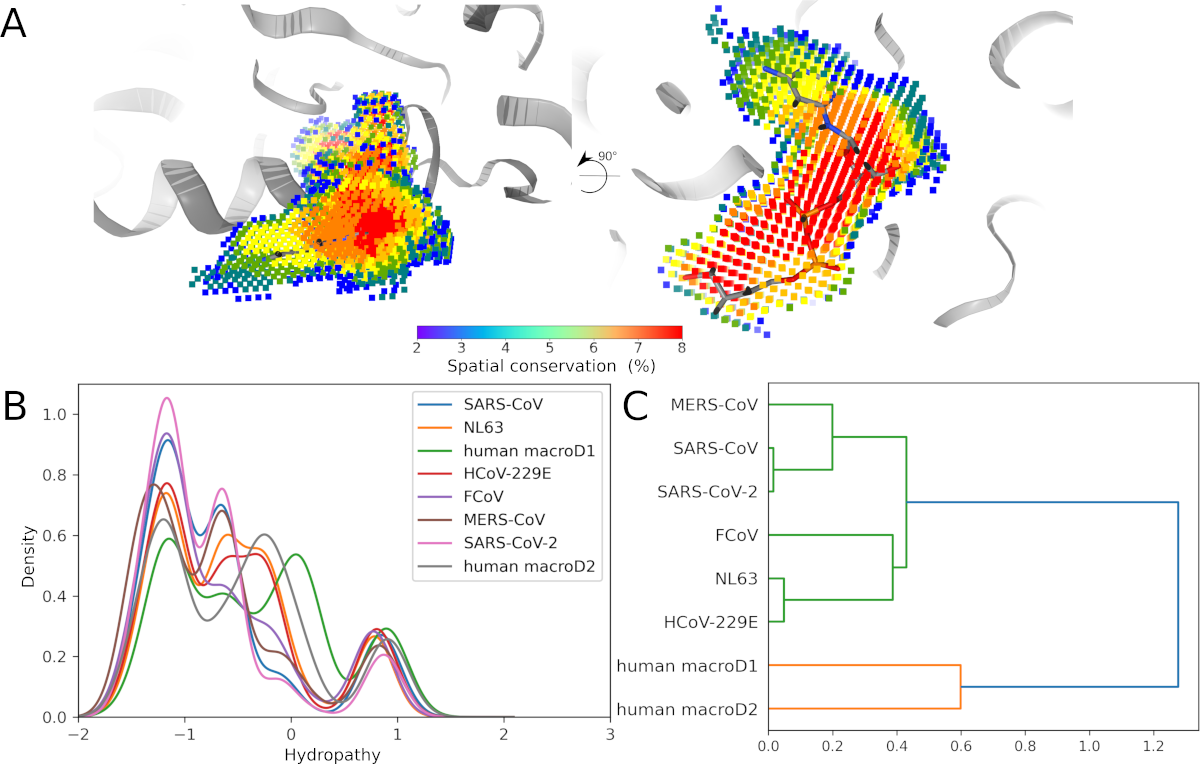
\includegraphics[scale=1]{images/adrp-sars-cov-2-conservation-analysis.png}
%   \centerline{\tiny{\textbf{Fonte:} Adaptado de \cite{guerra2021}.}}
%   \caption[Estudo do sítio de ligação do substrato da ADRP do SARS-CoV-2 e proteínas relacionadas]{\textbf{Estudo do sítio de ligação do substrato da ADRP do SARS-CoV-2 e proteínas relacionadas.} \textbf{(A)} Caracterizações do sítio de ligação do substrato do domínio ADRP do SARS-CoV-2 (PDB ID: 6WEN). Esquerda: Cavidade detectada representada como uma superfície cinza e os resíduos ao redor dela como \textit{sticks} vermelhos. Centro: Cavidade colorida por profundidade. Direita: Cavidade colorida por hidropatia usando a escala de Eisenberg e Weiss. \textbf{(B)} Gráfico de barras das frequências de resíduos de interface. Esquerda: Aminoácidos. Direita: Classes de aminoácidos. \textbf{(C)} Análise de conservação do sítio de ligação do ADP-ribose no domínio ADRP do SARS-CoV-2 (PDB ID: 6WEN, cadeia A), SARS-CoV (PDB ID: 2ACF, cadeia B), MERS-CoV (PDB ID: 5HIH, cadeia A), NL63 (PDB ID: 2VRI, cadeia A), HCoV-229E (PDB ID: 3EJG, cadeia A), FCoV (PDB ID: 3ETI, cadeia B) e proteínas macrodomínio macroD1 (PDB ID: 2X47, cadeia A) e macroD2 (PDB ID: 6Y73, cadeia D) humanas. Os pontos de cavidade que foram detectados em pelo menos duas estruturas e os pontos são coloridos por porcentagem de conservação. \textbf{(D)} Perfil de hidropatia. \textbf{(E)} Dendrograma de agrupamento hierárquico da frequência de resíduos. A métrica de correlação de Pearson foi usada para avaliar a similaridade e o método completo foi escolhido como método de ligação. Todos os gráficos e imagens foram gerados em um Jupyter notebook. As imagens das estruturas tridimensionais foram geradas utilizando o pacote NGLView \cite{nglview} enquanto os gráficos foram construídos utilizando o pacote matplotlib \cite{matplotlib}.}
%   \label{fig:conservation-analysis}
% \end{figure}

% Para comparar a composição dessa cavidade com a de outras proteínas relacionadas, realizamos a mesma análise em sete outras proteínas selecionadas com base em homologia estrutural e alinhamento utilizando o Dali \cite{dali}. As estruturas na forma apo foram realinhadas usando o algoritmo MUSTANG \cite{mustang} do programa YASARA \cite{yasara}. Ao aplicarmos operações aritméticas nas matrizes das cavidades detectadas, determinamos a conservação da cavidade entre as espécies. Conforme observado na Figura \ref{fig:conservation-analysis}C, o núcleo da cavidade da ADRP (pontos vermelhos) é altamente conservado nas espécies analisadas, estando ocupado pelo difosfato e ribose do ADP, bem como pela segunda ribose ligada ao ADP na forma ligada ao substrato da ADRP. Por outro lado, a adenosina ocupa uma região da cavidade menos conservada (pontos azuis), o que pode indicar que a estrutura desse sítio sofre alterações em algumas espécies para acomodar o substrato ADP-ribose.

% Para comparar a hidrofobicidade da cavidade entre as espécies, plotamos uma distribuição da hidrofobicidade usando a biblioteca matplotlib \cite{matplotlib}, conforme mostrado na Figura \ref{fig:conservation-analysis}D. A distribuição revela claramente a natureza hidrofóbica do bolsão, que é amplamente compartilhada entre as cavidades de ligação a substrato da ADRP dos coronavírus. Interessantemente, as proteínas humanas macroD1 e macroD2 parecem apresentar uma distribuição de hidrofobicidade menos pronunciada.

% Com o pyKVFinder, é possível calcular facilmente a frequência dos resíduos que compõem a cavidade. Utilizando a biblioteca SciPy\cite{scipy}, realizamos um agrupamento (\textit{clustering}, em inglês) hierárquico dessas frequências e apresentamos o dendrograma na Figura \ref{fig:conservation-analysis}E. Nesse dendrograma, observamos que a cavidade da ADRP do SARS-CoV-2 agrupa-se com a do SARS-CoV, o que demonstra alta similaridade entre esses betacoronavírus. Próximo a eles, podemos observar outro betacoronavírus, o MERS-CoV. Por sua vez, os alphacoronavírus NL63 e HCoV-229E e o feline FCoV agrupam-se juntos. Mais distantes dos domínios dos coronavírus, encontram-se as duas proteínas humanas macrodomínio, macroD1 e D2. Apesar da cavidade da ADRP ou macroD1/D2 compartilharem o mesmo substrato, o ADP-ribose, esses resultados indicam que o perfil dos resíduos ao redor dessas cavidades segue traços evolutivos.

% Para demonstrar as funcionalidades e vantagens do pyKVFinder, realizamos esse estudo em um \textit{Jupyter notebook}, onde executamos passo a passo as funções do pyKVFinder. O notebook com o caso de estudo completo está disponível em \url{https://github.com/LBC-LNBio/pyKVFinder/blob/master/examples/conservation-analysis/conservation-analysis.ipynb}. Uma descrição detalhada dessa análise está disponível no artigo publicado no periódico \textit{BMC Bioinformatics} \cite{guerra2021}. 

% \subsection{Dinâmica molecular do domínio ADRP do SARS-CoV-2}

% Nesse contexto, o desempenho computacional do pyKVFinder foi avaliado em simulações de DM do domínio ADRP do SARS-CoV-2 (PDB ID: 6W02, cadeia B) sem seu ligante, a ADP-ribose, por um período de 600 ns, com extração de quadros a cada 1 ns. Essa análise foi repetida com outras ferramentas bem conhecidas: parKVFinder \cite{guerra2020}, POVME \cite{povme}, fpocket \cite{fpocket}, GHECOM \cite{ghecom}, MSPocket \cite{mspocket} e Biobb\_vs \cite{biobbvs}. Todos esses métodos detectaram com sucesso o sítio de ligação do substrato da ADRP, no qual a forma e o volume variam ligeiramente durante a simulação de DM (Figura \ref{fig:pykvfinder-benchmarking}). A forma das cavidades detectadas pelo pyKVFinder e parKVFinder ajustam-se precisamente ao ligante original no sítio de ligação, assim como o MSPocket (Figura \ref{fig:pykvfinder-benchmarking}A). Além disso, o volume calculado pelo pyKVFinder ($346,8 \pm 78,7 \mAA^3$) e parKVFinder ($346,5 \pm 79,3 \mAA^3$) está intimamente relacionado ao volume da ADP-ribose ($351,1 \mAA^3$; volume da superfície molecular estimado pelo programa YASARA \cite{yasara}), o ligante que originalmente ocupava o sítio de ligação na estrutura cristalográfica utilizada nas simulações de DM (Figura \ref{fig:pykvfinder-benchmarking}B).

% \begin{figure}[h]
%   \centering
%   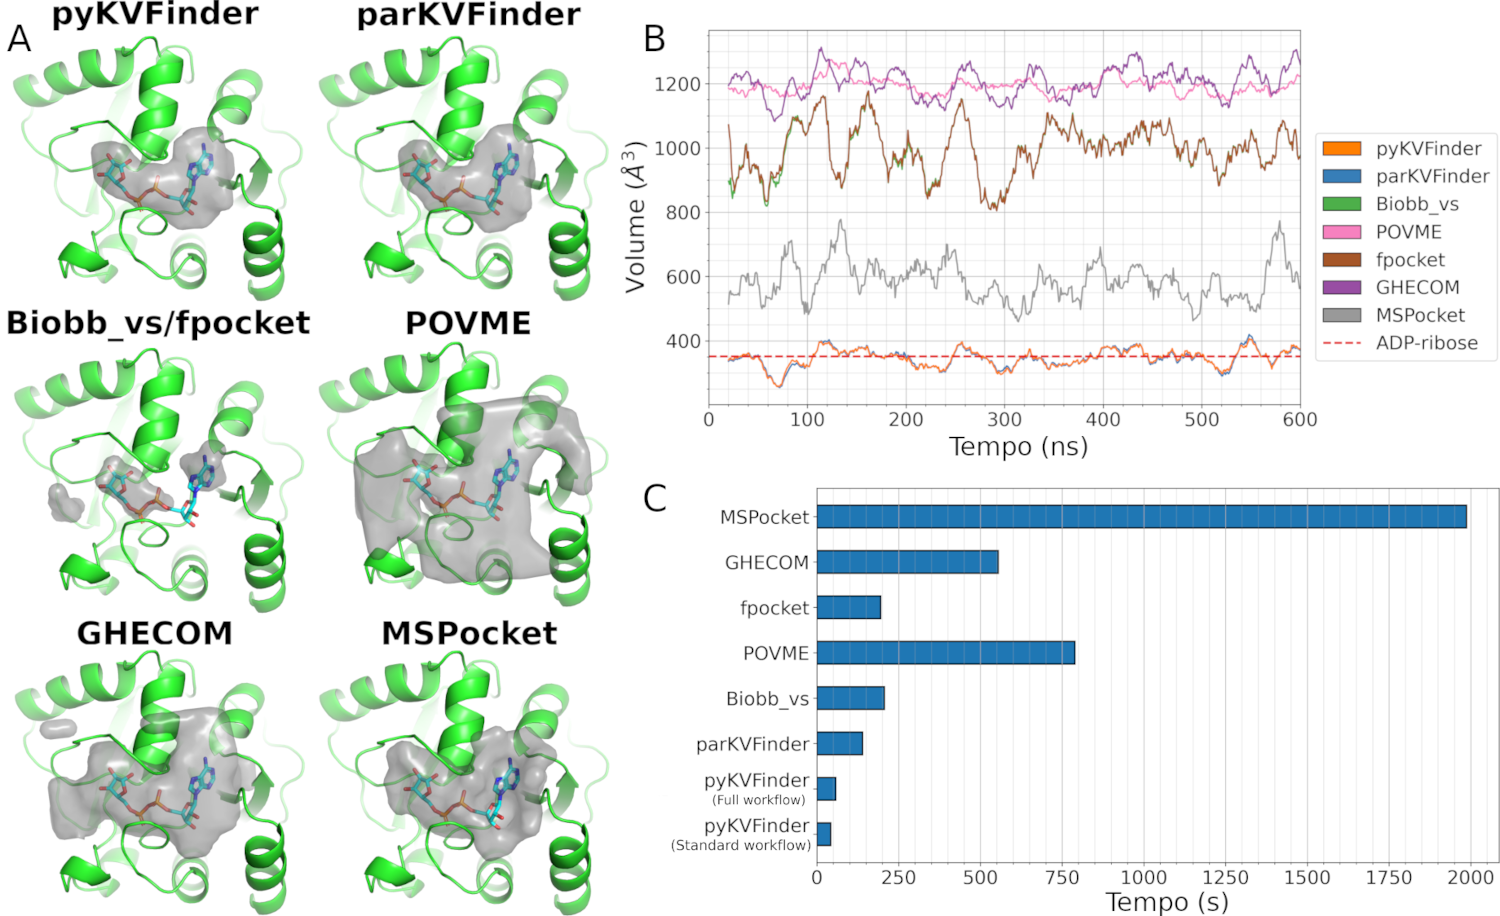
\includegraphics[scale=0.9]{images/pykvfinder-benchmarking.png}
%   \centerline{\tiny{\textbf{Fonte:} Adaptado de \cite{guerra2021}.}}
%   \caption[Avaliação de desempenho dos métodos de benchmarking para detecção do sítio de ligação do substrato da ADRP]{\textbf{Avaliação de desempenho dos métodos de benchmarking para detecção do sítio de ligação do substrato da ADRP.} \textbf{(A)} As estruturas da proteína (representadas em verde) no quadro 30 (com menor RMSD em comparação com a estrutura cristalográfica) da trajetória do domínio ADRP com as cavidades correspondentes detectadas (superfícies cinzas) por cada método de benchmarking. \textbf{(B)} O volume total das cavidades detectadas no sítio de ligação do substrato da ADRP ao longo da simulação de 600 ns. O volume total é calculado em uma janela de 20 quadros. A linha pontilhada vermelha indica o volume da superfície molecular da molécula de ADP-ribose, que ocupava originalmente o sítio de ligação do substrato da ADRP na estrutura cristalográfica (PDB ID: 6W02, cadeia B). \textbf{(C)} Tempo decorrido para detectar e caracterizar o sítio de ligação do substrato da ADRP. O protocolo padrão do pyKVFinder, assim como do parKVFinder, detecta as cavidades e aplica as caracterizações morfológicos (\eg, volume, área e forma) e topológicos (\eg, resíduos de interface e suas frequências). O protocolo completo do pyKVFinder inclui o protocolo padrão com as caracterizações de profundidade e hidropatia.}
%   \label{fig:pykvfinder-benchmarking}
% \end{figure}

% Além de ser capaz de detectar com acurácia cavidades biomoleculares, as ferramentas atuais também devem ter um desempenho rápido na detecção e caracterização dessas cavidades. Portanto, também avaliamos o tempo decorrido para executar esses métodos de benchmarking (Figura \ref{fig:pykvfinder-benchmarking}C). O pyKVFinder superou todos os métodos analisados nesse aspecto, até mesmo ao aplicar as novas características de caracterização, profundidade e hidropatia, o tempo decorrido do pyKVFinder aumentou apenas 36\%, ainda superando os outros métodos de \textit{benchmarking}. Além disso, em comparação ao parKVFinder, o pyKVFinder foi 3,3 vezes mais rápido na detecção do sítio de ligação da ADRP. A principal razão para o ganho de desempenho é a possibilidade adicional de paralelizar rotinas, ou seja, a inserção de átomos na grade 3D na função de detecção, com base em \textit{ndarrays}. Além disso, a escalabilidade do pyKVFinder, ao aumentar o número de threads, segue o mesmo comportamento apresentado pelo parKVFinder \cite{guerra2020}. Portanto, o pyKVFinder oferece uma opção mais flexível e eficiente para usuários experientes que precisam de aplicações em larga escala, enquanto o parKVFinder é mais adequado para iniciantes devido à sua simplicidade de instalação e uso.

% Para demonstrar as funcionalidades e vantagens do pyKVFinder, realizamos esse estudo em um \textit{Jupyter notebook}, onde executamos passo a passo as funções do pyKVFinder. O notebook com o caso de estudo completo está disponível em \url{https://github.com/LBC-LNBio/pyKVFinder/blob/master/examples/md-analysis/md-analysis.ipynb}. Uma descrição detalhada dessa análise está disponível no artigo publicado no periódico \textit{BMC Bioinformatics} \cite{guerra2021}.

% \section{KVFinder-web \label{ap:casos-de-estudo-kvfinder-web}}

% \subsection{Caracterização do sítio catalítico da protease do HIV-1}

% Como exemplo ilustrativo do KVFinder-web (Figura \ref{fig:kvweb-case-study}), detectamos e caracterizamos o sítio catalítico da protease do vírus da imunodeficiência humana tipo 1 (HIV-1) ligado ao oxigênio carbonílico de ureia cíclica \cite{lam1994}, utilizando o KVFinder-web portal. Conseguimos detectar com sucesso as cavidades em toda a superfície molecular da protease do HIV-1 (Figura \ref{fig:kvweb-case-study}A). Além da detecção de cavidades e definição de sua forma, o KVFinder-web também fornece o volume, área, profundidade e hidropatia das cavidades detectadas (Figura \ref{fig:kvweb-results}B; cavidade KAG). Normalmente, o sítio ativo é a maior e mais profunda cavidade na proteína enzimática \cite{laskowski1996}, e isso também é observado na protease do HIV-1, como mostrado na Figura \ref{fig:kvweb-results}B. Nesse sentido, a caracterização da profundidade pode ajudar os pesquisadores a identificarem o sítio ativo em toda a superfície molecular. Além disso, realizamos uma análise do perfil de hidrofobicidade do sítio ativo da protease do HIV-1 (Figura \ref{fig:kvweb-case-study}C). Nossos resultados mostraram que o sítio ativo é predominantemente hidrofóbico, especialmente na região próxima aos \textbeta-hairpins, e há poucas regiões hidrofílicas ao redor dos ácidos aspárticos catalíticos (Asp-25 e Asp-25'). Conforme esperado, os subsítios S1 e S1' (região amarela) são hidrofóbicos, e os subsítios S2 e S2' são predominantemente hidrofóbicos (região amarela), exceto por Asp-29 e Asp-30 (região azul). Além disso, observamos que a parte hidrofóbica dos subsítios S2 e S2', que acomodam os substratos P2 e P2', respectivamente, tendem a favorecer cadeias laterais alifáticas \cite{lam1994,brik2002,weber2009}.

% \begin{figure}[hp]
%   \centering
%   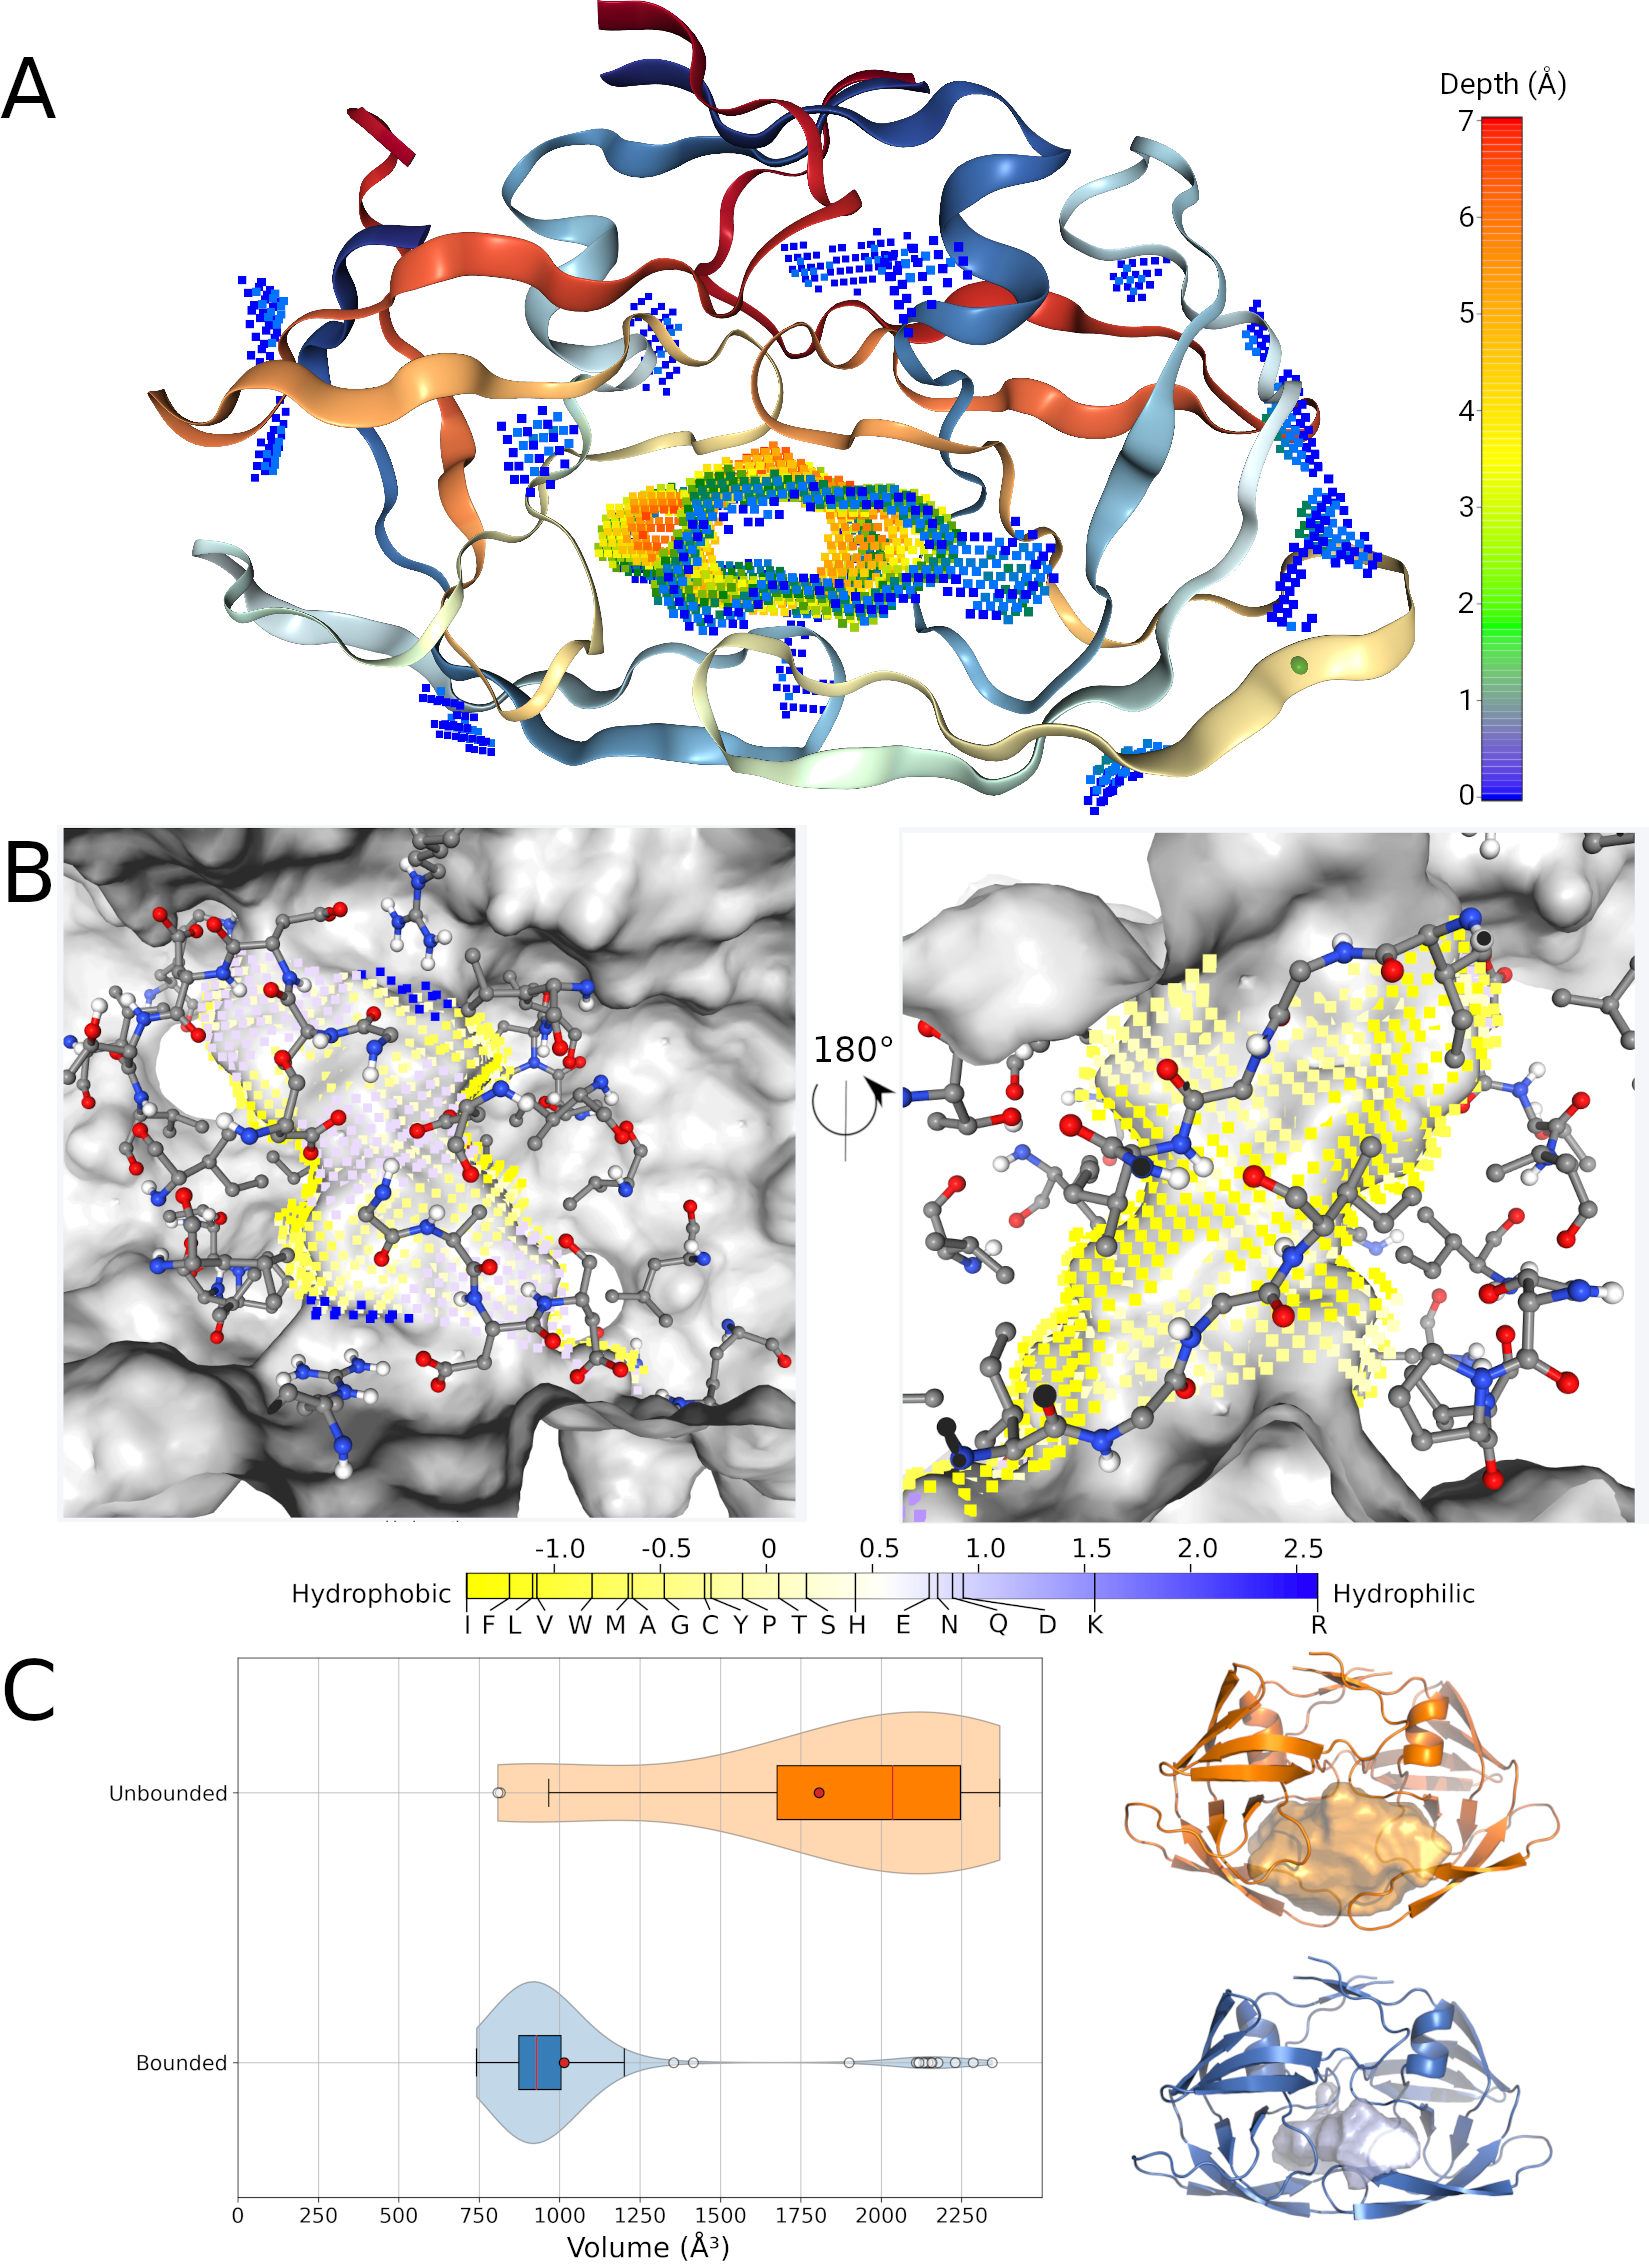
\includegraphics[scale=1.8]{images/kvweb-case-study.png}
%   \centerline{\tiny{\textbf{Fonte:} Adaptado de \cite{guerra2023A}.}}
%   \caption[Exemplo ilustrativo da detecção de cavidades na protease do HIV-1]{\textbf{Exemplo ilustrativo da detecção de cavidades na protease do HIV-1.} Estrutura molecular da protease do HIV-1 (PDB ID: 1HVR) com cavidades detectadas. \textbf{(A)} Detecção de cavidades em toda a estrutura da proteína (modelo em cartoon). Os pontos das cavidades são coloridos de acordo com a profundidade (pontos coloridos em uma escala de cores arco-íris). \textbf{(B)} Hidropatia mapeada nos pontos de cavidade na superfície nas regiões ao redor dos ácidos aspárticos catalíticos (painel esquerdo) e ao redor dos β-hairpins (painel direito). A escala de hidrofobicidade de Eisenberg & Weiss varia de -1,42 (altamente hidrofóbica) a 2,6 (altamente hidrofílica). A proteína é mostrada como uma superfície cinza e os resíduos de interface são mostrados como átomos coloridos em sticks. \textbf{(C)} Gráfico de violino do volume do sítio ativo das estruturas da protease do HIV-1 do RCSB PDB para as estruturas com ligantes ligados no sítio ativo (azul) e as estruturas sem ligantes (laranja). As estruturas com uma mediana de volume e a cavidade correspondente são mostradas como modelo em cartoon e superfície, respectivamente.}
%   \label{fig:kvweb-case-study}
% \end{figure}

% \subsection{Comparação morfológica do sítio catalítico das estruturas da protease do HIV-1}

% Conforme apresentado na Seção \ref{sec:md-hiv1-protease}, a protease do HIV-1 é um alvo terapêutico eficaz, o sítio catalítico é o alvo de diversos medicamentos antirretrovirais. No entanto, o ciclo catalítico depende dos movimentos dos \textbeta-hairpins, que controlam a acessibilidade dos substratos ao sítio ativo \cite{lam1994,soares2016}. Assim, analisamos as estruturas da protease do HIV-1 disponíveis no PDB e comparamos suas cavidades (consulte \cite{guerra2023A}). Com base nos volumes das cavidades, é possível diferenciar claramente as estruturas nas formas ligada das não-ligadas (Figura \ref{fig:kvweb-case-study}C), indicando uma complementaridade geométrica entre receptor e ligantes, juntamente com uma complementaridade físico-química, mostrada pelo perfil de hidrofobicidade discutido anteriormente.

% % \section{KVFinderMD}

% % \subsection{Estudo comparativo dos sítios de ligação do substrato da ALDH1 e ALDH2}

% % o caso das ALDH1/2, exploramos as diferenças topológicas e volumétricas entre os sítios de ligação do substrato de ALDH1 e ALDH2, o que dita a preferência por aldeídos menores e maiores entre eles.

% \chapter{Figuras suplementares \label{ap:figuras-suplementares}}

% \begin{figure}[htb]
%   \centering
%   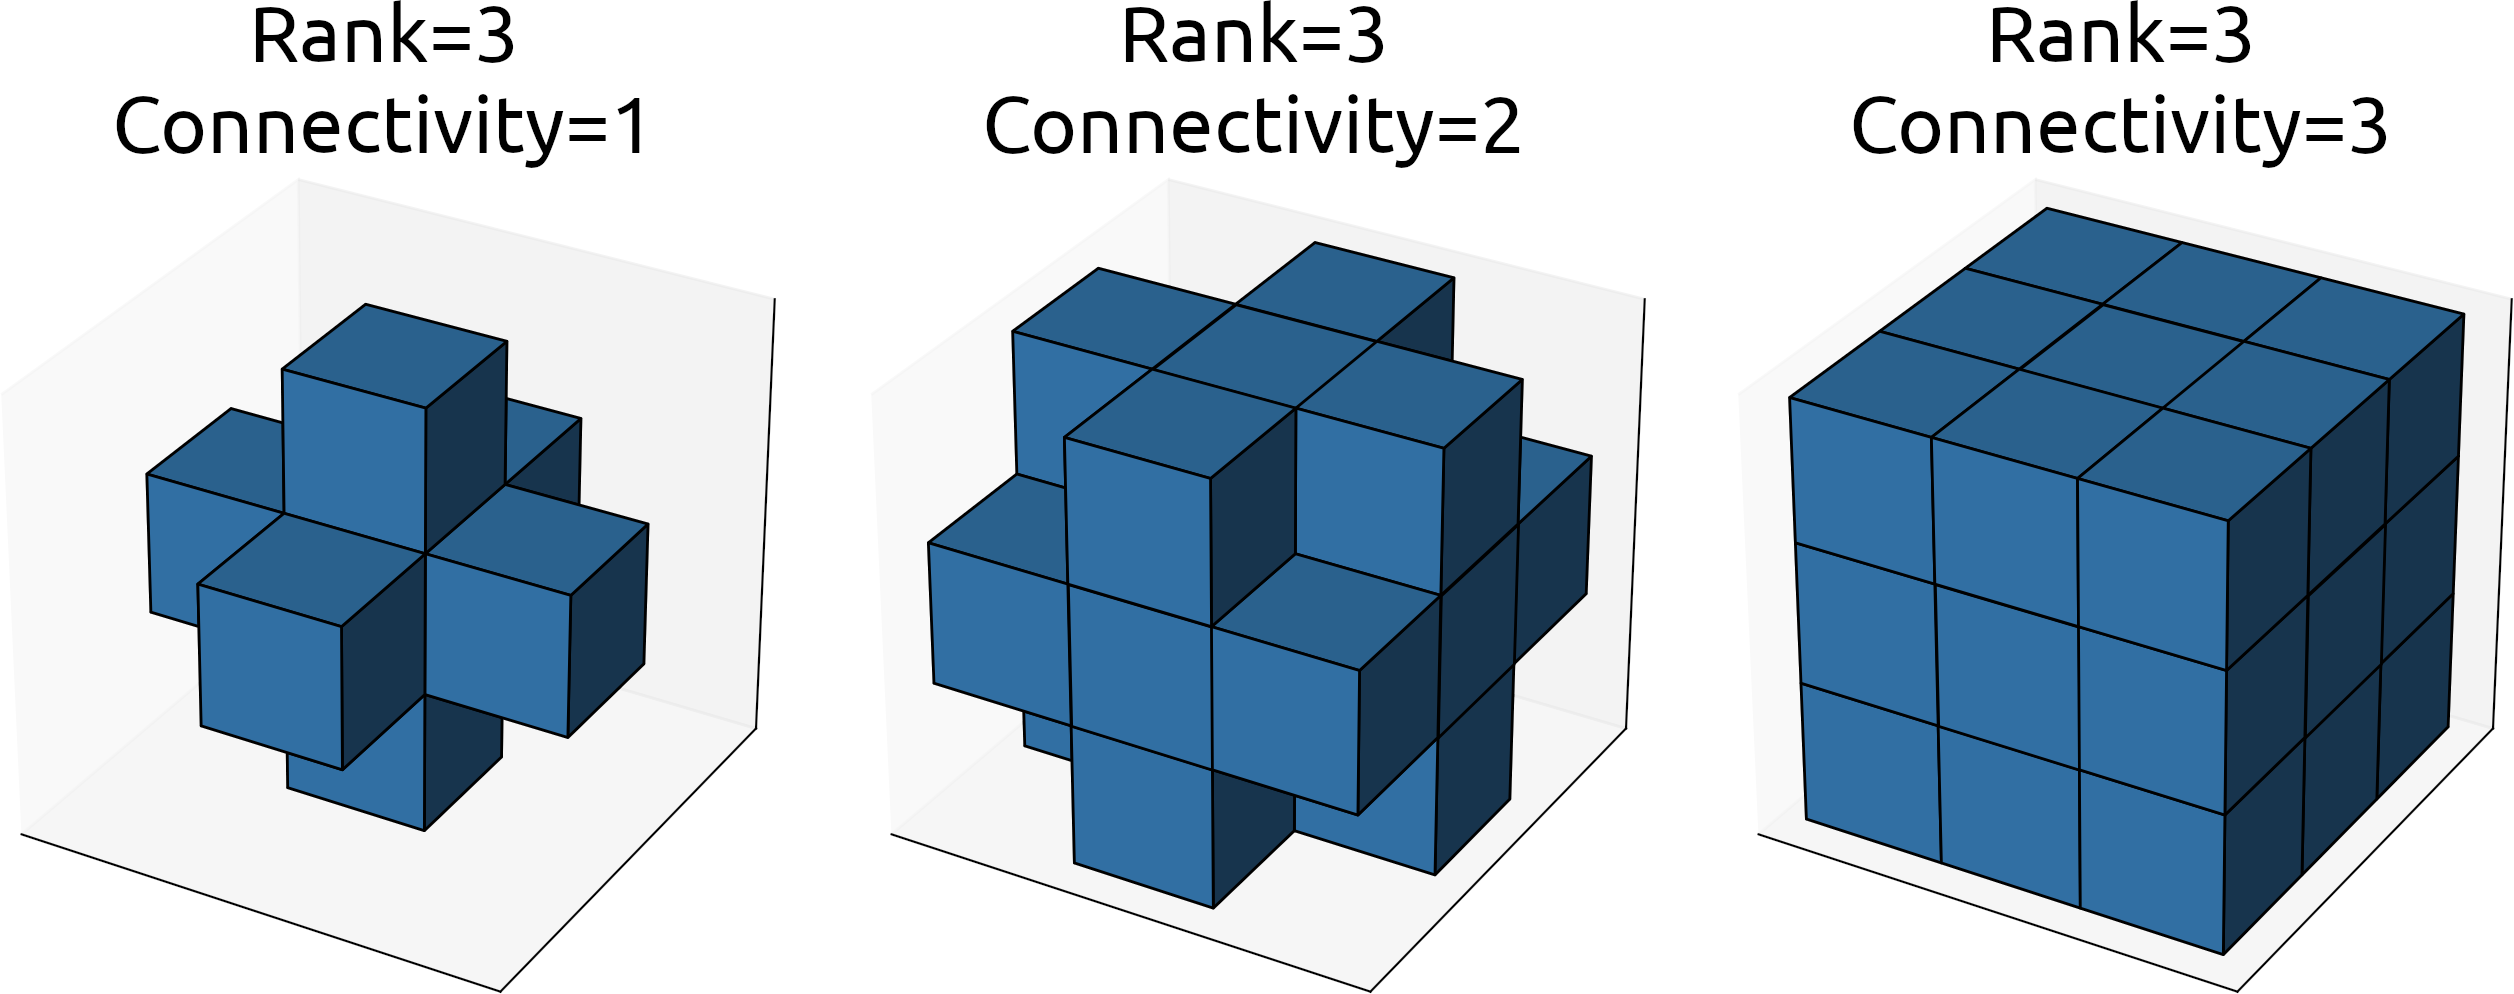
\includegraphics[scale=1]{images/3D-binary-structure.png}
%   \centerline{\tiny{\textbf{Fonte:} Retirado de \url{https://docs.scipy.org/doc/scipy/tutorial/ndimage.html}}}
%   \caption[Elementos estruturantes para filtros espaciais]{\textbf{Elementos estruturantes para filtros espaciais.}}
%   \label{fig:elementos-estruturantes}
% \end{figure}

\end{document}
